Objectifs du cours

Utiliser des démarches et des méthodes permettant de décrire et de
caractériser les mouvements (trajectoire, vitesse et accélération) de
tous les points des solides d'un système.

Savoirs

\textbf{Je connais~:}

\begin{longtable}{@{}
  >{\raggedright\arraybackslash}p{(\columnwidth - 2\tabcolsep) * \real{0.9045}}
  >{\raggedright\arraybackslash}p{(\columnwidth - 2\tabcolsep) * \real{0.0955}}@{}}
\toprule\noalign{}
\begin{minipage}[b]{\linewidth}\raggedright
\begin{itemize}
\item
  les~définitions des vecteurs position, vitesse et accélération;
\end{itemize}
\end{minipage} & \begin{minipage}[b]{\linewidth}\raggedright
$\bigcirc$
\end{minipage} \\
\midrule\noalign{}
\endhead
\bottomrule\noalign{}
\endlastfoot
\begin{minipage}[t]{\linewidth}\raggedright
\begin{itemize}
\item
  la relation de composition des vecteurs vitesse~;
\end{itemize}
\end{minipage} & $\bigcirc$ \\
\begin{minipage}[t]{\linewidth}\raggedright
\begin{itemize}
\item
  la relation de composition des vecteurs rotation~;
\end{itemize}
\end{minipage} & $\bigcirc$ \\
\begin{minipage}[t]{\linewidth}\raggedright
\begin{itemize}
\item
  la relation de composition des torseurs cinématiques;
\end{itemize}
\end{minipage} & $\bigcirc$ \\
\begin{minipage}[t]{\linewidth}\raggedright
\begin{itemize}
\item
  la relation du champ des vecteurs vitesse d'un solide;
\end{itemize}
\end{minipage} & $\bigcirc$ \\
\begin{minipage}[t]{\linewidth}\raggedright
\begin{itemize}
\item
  connaître la loi trapèze.
\end{itemize}
\end{minipage} & $\bigcirc$ \\
\end{longtable}

Savoir-faire

\textbf{Je sais~:}

\begin{longtable}{@{}
  >{\raggedright\arraybackslash}p{(\columnwidth - 2\tabcolsep) * \real{0.9045}}
  >{\raggedright\arraybackslash}p{(\columnwidth - 2\tabcolsep) * \real{0.0955}}@{}}
\toprule\noalign{}
\begin{minipage}[b]{\linewidth}\raggedright
\begin{itemize}
\item
  nommer un mouvement~;
\end{itemize}
\end{minipage} & \begin{minipage}[b]{\linewidth}\raggedright
$\bigcirc$
\end{minipage} \\
\midrule\noalign{}
\endhead
\bottomrule\noalign{}
\endlastfoot
\begin{minipage}[t]{\linewidth}\raggedright
\begin{itemize}
\item
  décrire la trajectoire d'un point appartenant à un solide en
  mouvement~;~
\end{itemize}
\end{minipage} & $\bigcirc$ \\
\begin{minipage}[t]{\linewidth}\raggedright
\begin{itemize}
\item
  déterminer le vecteur position d'un point appartenant à un solide en
  mouvement~~;~
\end{itemize}
\end{minipage} & $\bigcirc$ \\
\begin{minipage}[t]{\linewidth}\raggedright
\begin{itemize}
\item
  exprimer un vecteur rotation~;~
\end{itemize}
\end{minipage} & $\bigcirc$ \\
\begin{minipage}[t]{\linewidth}\raggedright
\begin{itemize}
\item
  dériver, par rapport au temps, un vecteur dans un repère;
\end{itemize}
\end{minipage} & $\bigcirc$ \\
\begin{minipage}[t]{\linewidth}\raggedright
\begin{itemize}
\item
  déterminer, à l'aide de deux méthodes, le vecteur vitesse d'un point
  appartenant à un solide en mouvement~;
\end{itemize}
\end{minipage} & $\bigcirc$ \\
\begin{minipage}[t]{\linewidth}\raggedright
\begin{itemize}
\item
  déterminer le vecteur accélération d'un point appartenant à un solide
  en mouvement~;
\end{itemize}
\end{minipage} & $\bigcirc$ \\
\begin{minipage}[t]{\linewidth}\raggedright
\begin{itemize}
\item
  déterminer les évolutions de la position, vitesse, accélération pour
  une loi de vitesse en trapèze.
\end{itemize}
\end{minipage} & $\bigcirc$ \\
\end{longtable}

\subsection{MISE EN SITUATION}\label{mise-en-situation}

\subsubsection{Cas n°1~: Lenteur d'un robot de
chirurgie}\label{cas-n1-lenteur-dun-robot-de-chirurgie}

Même si elle n'est pas encore aussi répandue en France qu'aux
Etats-Unis, la chirurgie robotique se développe peu à peu. Son usage
nécessite la maîtrise de la machine et une familiarisation avec sa
manipulation, mais aussi une prise en compte des contraintes qu'elle
impose, notamment sur la durée de l'intervention. L'absence de
précautions particulières peut être source de responsabilité. C'est ce
que rappelle un arrêt de la cour administrative d'appel de Lyon du 29
septembre 2016.

Il apparaît ainsi que l'usage du robot est en lien de causalité direct
et certain avec les dommages du fait de l'allongement de la durée de
l'intervention, due à la fois aux nécessités d'installation du robot et
à son maniement « hésitant » par l'opérateur.


\includegraphics[width=\linewidth,height=.72\textheight,keepaspectratio]{images/image5.jpeg}

Pour des nombreux systèmes, en particulier pour ceux du domaine de la
robotique industrielle ou grand public, un des principaux enjeux de leur
concepteur est de faire en sorte qu'ils respectent parfaitement la
\textbf{cinématique} imposée par leur cahier des charges. Il s'agit de
s'assurer que les \textbf{mouvements} des pièces qui les constituent
s'exécutent parfaitement suivant des \textbf{directions} et à des
\textbf{vitesses maitrisées}.

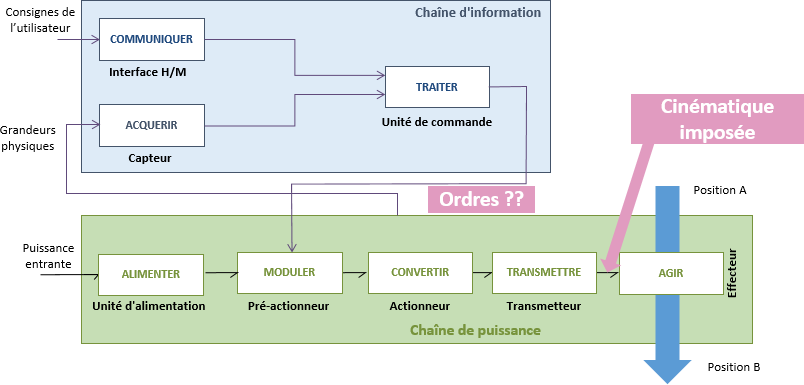
\includegraphics[width=\linewidth,height=.72\textheight,keepaspectratio]{images/image6.png}On
parle alors des \textbf{lois de commande en mouvement} d'un
\textbf{mécanisme} qui doivent permettre, comme finalité, d'établir des
\textbf{relations} entre les \textbf{ordres} envoyés par l'unité de
commande aux pré-actionneurs des chaînes d'énergie- puissance et la
\textbf{cinématique imposée aux effecteurs} par le cahier des charges du
système.

\subsubsection[Cas n°2~: Prothèse
transtibiale]{\texorpdfstring{\protect
\includegraphics[width=\linewidth,height=.72\textheight,keepaspectratio]{images/image7.jpeg}Cas
n°2~: Prothèse
transtibiale}{Cas n°2~: Prothèse transtibiale}}\label{cas-n2-prothuxe8se-transtibiale}

La prothèse transtibiale doit permettre à la personne de réaliser les
mêmes mouvements qu'un pied réel, que ce soit en termes d'amplitudes, de
vitesse ou d'accélération.

Pour maitriser les positions et les vitesses, il faut pouvoir modéliser
les différents mouvements du mécanisme~!

'\,'

\subsection{~INTRODUCTION CINEMATIQUE}\label{introduction-cinematique}

\subsubsection{Définitions et
hypothèses}\label{duxe9finitions-et-hypothuxe8ses}

La cinématique est une théorie partielle de la mécanique qui a pour but
la description des mouvements des systèmes mécaniques, indépendamment
des causes qui les produisent. En d'autres termes, la cinématique
cherche à décrire les mouvements et non à les expliquer. L'objectif de
la cinématique est donc d'utiliser des démarches et des méthodes
permettant de \emph{\textbf{décrire}} et de \emph{\textbf{caractériser
les mouvements de tous les points des solides}} d'un système.

Lors de l'utilisation d'un système, les solides qui le constituent se
déforment sous l'action des efforts qu'ils subissent. Dans la suite, on
fera l'hypothèse que ces déformations sont suffisamment petites pour que
l'on puisse les négliger et on~considérera les \emph{\textbf{solides}}
comme étant \emph{\textbf{indéformables}} (sont donc exclus les solides
dont la fonction est de se déformer comme les ressorts, barres de
torsion,\ldots).

Cela implique que la distance entre deux points A et B d'un même solide
1 ne varie pas au cours du temps~:
\(\forall t,\mspace{6mu}\forall A \in 1,\mspace{6mu}\forall B \in 1,\quad\left\| \overrightarrow{AB} \right\| = Cte\)

\subsubsection{Base, repère et
référentiel}\label{base-repuxe8re-et-ruxe9fuxe9rentiel}

\textbf{Une base} de l'espace vectoriel réel de dimension 3 est un
ensemble de trois vecteurs non coplanaires que nous noterons
\(\overrightarrow{\text{x}}\)\textbf{,}
\(\overrightarrow{\text{y}}\)\textbf{,} \(\overrightarrow{\text{z}}\).

\textbf{Un repère d'espace} de l'espace affine usuel de dimension 3 est
un ensemble composé d'un point nommé origine, que nous noterons O, et
d'une base \(\overrightarrow{\text{x}}\), \(\overrightarrow{\text{y}}\),
\(\overrightarrow{\text{z}}\). Le repère sera noté (O,
\(\overrightarrow{\text{x}}\), \(\overrightarrow{\text{y}}\),
\(\overrightarrow{\text{z}}\)).

Un \textbf{repère de temps} est constitué d'un instant d'origine et
d'une échelle de temps.

Un \textbf{référentiel} est un ensemble constitué d'un repère d'espace
et d'un repère de temps.

\ul{Remarque~:} dans les problèmes de SII, le temps est le même pour
tous les référentiels. En d'autres termes les changements de
référentiels se borneront à des changements d'espace géométrique. Par
abus de langage le mot référentiel est souvent remplacé par repère de
référence voire tout simplement par repère.

\emph{\textbf{Dans la suite, on parlera indifféremment d'un solide ou du
repère qui lui est attaché}}

\subsubsection[Définition du produit
vectoriel]{\texorpdfstring{\protect
\includegraphics[width=\linewidth,height=.72\textheight,keepaspectratio]{images/image10.jpeg}Définition
du produit
vectoriel}{Définition du produit vectoriel}}\label{duxe9finition-du-produit-vectoriel}

Le produit vectoriel de deux vecteurs \(\overrightarrow{U}\) et
\(\overrightarrow{V}\) est un vecteur noté
\(\overrightarrow{U} \land \overrightarrow{V}\) tel que :

\begin{itemize}
\item
  
\includegraphics[width=\linewidth,height=.72\textheight,keepaspectratio]{images/image11.jpeg}
\includegraphics[width=\linewidth,height=.72\textheight,keepaspectratio]{images/image12.jpeg}
  \(\overrightarrow{U} \land \overrightarrow{V}\)soit perpendiculaire au
  plan (\(\overrightarrow{U}\), \(\overrightarrow{V}\))~;
\item
  Le trièdre (\(\overrightarrow{U}\), \(\overrightarrow{V}\),
  \(\overrightarrow{U} \land \overrightarrow{V}\))~est direct.
\item
  \(\left\| \overrightarrow{U} \land \overrightarrow{V} \right\| = \left\| \overrightarrow{U} \right\|.\left\| \overrightarrow{V} \right\|.\left| \sin\left( \overrightarrow{U},\overrightarrow{V} \right) \right|\)
\end{itemize}

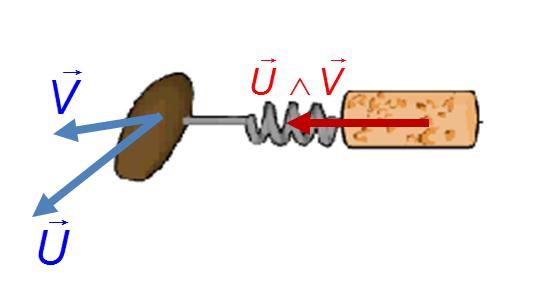
\includegraphics[width=\linewidth,height=.72\textheight,keepaspectratio]{images/image13.jpeg}\emph{\textbf{On
utilise aussi la règle du « tire bouchon »}}

Il faut imaginer le tire bouchon «~planté~» dans le bouchon :

\begin{itemize}
\item
  si on dévisse on sort le bouchon;
\item
  si on visse on rentre le bouchon.
\end{itemize}

\paragraph*{Pour les vecteurs unitaires d'une même
base}\label{pour-les-vecteurs-unitaires-dune-muxeame-base}
\addcontentsline{toc}{paragraph}{Pour les vecteurs unitaires d'une même
base}

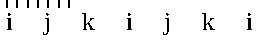
\includegraphics[width=\linewidth,height=.72\textheight,keepaspectratio]{images/image14.pdf}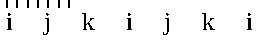
\includegraphics[width=\linewidth,height=.72\textheight,keepaspectratio]{images/image14.pdf}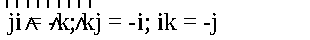
\includegraphics[width=\linewidth,height=.72\textheight,keepaspectratio]{images/image15.pdf}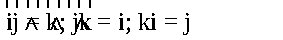
\includegraphics[width=\linewidth,height=.72\textheight,keepaspectratio]{images/image16.pdf}

\textbf{$\wedge$}

\textbf{+}

\textbf{$\wedge$}

\textbf{-}

\paragraph*{Propriétés}\label{propriuxe9tuxe9s}
\addcontentsline{toc}{paragraph}{Propriétés}

\begin{itemize}
\item
  \emph{antisymétrie
  :}\(\overrightarrow{U} \land \overrightarrow{V} = - \overrightarrow{V} \land \overrightarrow{U}\)
\item
  \emph{Distributivité par rapport à l'addition :}
  \(\overrightarrow{U} \land (\overrightarrow{V} + \overrightarrow{W}) = \overrightarrow{U} \land \overrightarrow{V} + \overrightarrow{U} \land \overrightarrow{W}\)
\item
  \emph{Multiplication par un réel :}
  \(\lambda.\overrightarrow{U} \land µ.\overrightarrow{V} = \lambda µ.(\overrightarrow{U} \land \overrightarrow{V})\)
\end{itemize}

\paragraph*{\texorpdfstring{\protect
\includegraphics[width=\linewidth,height=.72\textheight,keepaspectratio]{images/image17.jpeg}Cas
particulier}{Cas particulier}}\label{cas-particulier}
\addcontentsline{toc}{paragraph}{Cas particulier}

Le produit vectoriel est \textbf{nul} :

\begin{itemize}
\item
  Si un des deux vecteurs est nul
\item
  Si les 2 vecteurs sont \textbf{colinéaires}
\end{itemize}

\begin{longtable}{@{}
  >{\raggedright\arraybackslash}p{(\columnwidth - 2\tabcolsep) * \real{0.1227}}
  >{\raggedright\arraybackslash}p{(\columnwidth - 2\tabcolsep) * \real{0.8773}}@{}}
\toprule\noalign{}
\begin{minipage}[b]{\linewidth}\raggedright
\begin{quote}

\includegraphics[width=\linewidth,height=.72\textheight,keepaspectratio]{images/image18.png}
\end{quote}
\end{minipage} & \begin{minipage}[b]{\linewidth}\raggedright
\begin{enumerate}
\def\labelenumi{\arabic{enumi}.}
\item
  Calculer le produit vectoriel
  \(\overrightarrow{V_{1}} \land \overrightarrow{V_{2}}\) avec~:
\end{enumerate}

\(\overrightarrow{V_{1}} = (2.\overrightarrow{x} + 2.\overrightarrow{y} - 3.\overrightarrow{z})\mspace{6mu} et\mspace{6mu}\overrightarrow{V_{2}} = ( - \overrightarrow{x} + 6.\overrightarrow{z})\)
\end{minipage} \\
\midrule\noalign{}
\endhead
\bottomrule\noalign{}
\endlastfoot
\end{longtable}


\includegraphics[width=\linewidth,height=.72\textheight,keepaspectratio]{images/image19.png}

\paragraph*{\texorpdfstring{\protect
\includegraphics[width=\linewidth,height=.72\textheight,keepaspectratio]{images/image20.png}Produit
mixte}{Produit mixte}}\label{produit-mixte}
\addcontentsline{toc}{paragraph}{Produit mixte}

\((\overrightarrow{U},\overrightarrow{V},\overrightarrow{W}) = (\overrightarrow{U} \land \overrightarrow{V}) \bullet \overrightarrow{W}\)
est le produit mixte de trois vecteurs
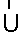
\includegraphics[width=\linewidth,height=.72\textheight,keepaspectratio]{images/image21.pdf},
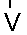
\includegraphics[width=\linewidth,height=.72\textheight,keepaspectratio]{images/image22.pdf} et
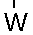
\includegraphics[width=\linewidth,height=.72\textheight,keepaspectratio]{images/image23.pdf} est le \textbf{nombre réel}
suivant noté
\((\overrightarrow{U}\text{,}\overrightarrow{\text{V}}\text{,}\overrightarrow{\text{W}})\)~:

\(\left| (\overrightarrow{U},\overrightarrow{V},\overrightarrow{W}) \right|\)
= volume parallépipède

Le produit mixte est invariant par permutation circulaire des trois
opérandes :

\[(\overrightarrow{U} \land \overrightarrow{V}) \bullet \overrightarrow{W} = (\overrightarrow{W} \land \overrightarrow{U}) \bullet \overrightarrow{V} = (\overrightarrow{V} \land \overrightarrow{W}) \bullet \overrightarrow{U}\]

La permutation de deux opérandes change le signe du produit mixte :

\((\overrightarrow{U} \land \overrightarrow{V}) \bullet \overrightarrow{W} = - (\overrightarrow{V} \land \overrightarrow{U}) \bullet \overrightarrow{W}\)

\subsubsection{Un peu d'entraînement}\label{un-peu-dentrauxeenement}

\begin{longtable}{@{}
  >{\raggedright\arraybackslash}p{(\columnwidth - 2\tabcolsep) * \real{0.1227}}
  >{\raggedright\arraybackslash}p{(\columnwidth - 2\tabcolsep) * \real{0.8773}}@{}}
\toprule\noalign{}
\begin{minipage}[b]{\linewidth}\raggedright
\begin{quote}

\includegraphics[width=\linewidth,height=.72\textheight,keepaspectratio]{images/image18.png}
\end{quote}
\end{minipage} & \begin{minipage}[b]{\linewidth}\raggedright
\begin{enumerate}
\def\labelenumi{\arabic{enumi}.}
\item
  
\includegraphics[width=\linewidth,height=.72\textheight,keepaspectratio]{images/image24.jpeg}Calculer
  les produits vectoriels suivant~:
\end{enumerate}

\[{\overrightarrow{x}}_{1} \land {\overrightarrow{z}}_{0} =\]

\[{\overrightarrow{y}}_{0} \land {\overrightarrow{z}}_{0} =\]

\[{\overrightarrow{x}}_{1} \land {\overrightarrow{y}}_{2} =\]

\[{\overrightarrow{z}}_{0} \land {\overrightarrow{z}}_{3} =\]

\[{\overrightarrow{y}}_{3} \land {\overrightarrow{x}}_{1} =\]

\[{\overrightarrow{y}}_{1} \land {\overrightarrow{y}}_{2} =\]

\[{\overrightarrow{z}}_{3} \land {\overrightarrow{x}}_{1} =\]

\[{\overrightarrow{x}}_{3} \land {\overrightarrow{y}}_{2} =\]

\[{\overrightarrow{x}}_{3} \land {\overrightarrow{x}}_{0} =\]

\[{\overrightarrow{y}}_{1} \land {\overrightarrow{y}}_{3} =\]

\[{\overrightarrow{z}}_{3} \land {\overrightarrow{y}}_{2} =\]

\[{\overrightarrow{y}}_{1} \land {\overrightarrow{x}}_{3} =\]

\[{\overrightarrow{x}}_{0} \land {\overrightarrow{y}}_{1} =\]

\[{\overrightarrow{y}}_{3} \land {\overrightarrow{y}}_{0} =\]
\end{minipage} \\
\midrule\noalign{}
\endhead
\bottomrule\noalign{}
\endlastfoot
\end{longtable}

\subsubsection{Torseur cinématique}\label{torseur-cinuxe9matique}

Le couple formé par \emph{\textbf{le vecteur rotation}}
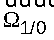
\includegraphics[width=\linewidth,height=.72\textheight,keepaspectratio]{images/image25.pdf}et le \emph{\textbf{vecteur
vitesse}} 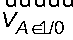
\includegraphics[width=\linewidth,height=.72\textheight,keepaspectratio]{images/image26.pdf} constitue le
\emph{\textbf{torseur cinématique}} du solide \emph{1} dans son
mouvement par rapport au solide \emph{0} et exprimé au point \emph{A}~:

\begin{longtable}{@{}
  >{\raggedright\arraybackslash}p{(\columnwidth - 2\tabcolsep) * \real{0.2717}}
  >{\raggedright\arraybackslash}p{(\columnwidth - 2\tabcolsep) * \real{0.7283}}@{}}
\toprule\noalign{}
\multirow{2}{=}{\begin{minipage}[b]{\linewidth}\raggedright
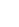
\includegraphics[width=\linewidth,height=.72\textheight,keepaspectratio]{images/image27.pdf}\(\left\{ V_{1/0} \right\} = \begin{Bmatrix}
\overrightarrow{\Omega_{1/0}} \\
\overrightarrow{V_{A \in 1/0}}
\end{Bmatrix}_{A}\)
\end{minipage}} & \begin{minipage}[b]{\linewidth}\raggedright
\(\overrightarrow{\Omega_{1/0}}\) est la \emph{\textbf{résultante
cinématique}} du torseur, indépendante du point choisi pour exprimer le
torseur.
\end{minipage} \\
& \begin{minipage}[b]{\linewidth}\raggedright
\(\overrightarrow{V_{A \in 1/0}}\) est le \emph{\textbf{moment
cinématique}} du torseur au point A.
\end{minipage} \\
\midrule\noalign{}
\endhead
\bottomrule\noalign{}
\endlastfoot
\end{longtable}

Ce torseur permet de définir le mouvement d'un solide par rapport à un
autre (ici 1/0).

\emph{Remarque~:}
\(\boxed{\left\{ V_{2/1} \right\} = - \left\{ V_{1/2} \right\}}\)\emph{.}

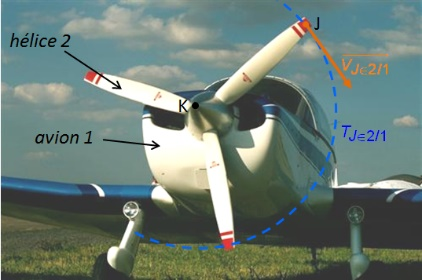
\includegraphics[width=\linewidth,height=.72\textheight,keepaspectratio]{images/image29.jpeg}\emph{\textbf{Exemple~:}}
\(\left\{ V_{2/1} \right\} = \begin{Bmatrix}
\overrightarrow{\Omega_{2/1}} \\
\overrightarrow{V_{J \in 2/1}}
\end{Bmatrix}_{J}\)

Quel que soit le point, l'hélice tourne à la même vitesse
\(\left\| \overrightarrow{\Omega_{2/1}} \right\|\). Par contre chaque
point à une vitesse différente que l'on peut déterminer si l'on connait
la vitesse en un point (par exemple~:
\(\overrightarrow{V_{K \in 2/1}} = \overrightarrow{0}\)).

\paragraph*{Définition d'un torseur}\label{duxe9finition-dun-torseur}
\addcontentsline{toc}{paragraph}{Définition d'un torseur}

On appelle torseur la réunion de deux vecteurs \(\overrightarrow{R}\) et
\({\overrightarrow{M}}_{A}\) \textbf{:}

\begin{itemize}
\item
  \(\overrightarrow{R}\) est la \textbf{résultante} \textbf{du torseur},
  elle est invariante du point où est exprimé le torseur~;
\item
  \({\overrightarrow{M}}_{A}\) est le \textbf{moment du torseur}, son
  expression dépend du point où il est exprimé (ici le point A).
\end{itemize}

Le torseur peut être écrit~:

\begin{itemize}
\item
  En ligne~: \(\left\{ T \right\} = \begin{Bmatrix}
  \overrightarrow{R} \\
  {\overrightarrow{M}}_{A}
  \end{Bmatrix}_{A}\) (dans ce cas-là les coordonnées des vecteurs
  peuvent être exprimées dans des bases différentes)
\item
  En colonnes~: \(\left\{ T \right\} = \left\{ \left. \ \begin{matrix}
  X \\
  Y \\
  Z
  \end{matrix} \right|\begin{matrix}
  L \\
  M \\
  N
  \end{matrix} \right\}_{\text{A,}\overrightarrow{\text{i}}\text{,}\overrightarrow{\text{j}}\text{,}\overrightarrow{\text{k}}}\)~,
  les coordonnées doivent être exprimées dans la base associée (ici
  \((\overrightarrow{i},\overrightarrow{j},\overrightarrow{k})\)). Les
  lettres X, Y, Z, L, M et N sont utilisées pour la représentation
  d'efforts, donc \textbf{uniquement} pour le torseur des actions
  mécaniques transmissibles.
\end{itemize}

\textbf{Remarque~:} on parle de composantes ou de coordonnées
plückériennes du torseur.

On parle de « \textbf{résultante »} et de « \textbf{moment »} pour tous
les torseurs, pas uniquement pour le torseur des actions mécaniques ! La
résultante et le moment sont appelés \textbf{éléments de réduction} du
torseur.

Il est possible d'avoir les résultantes et les moments dans des bases
différentes exprimés ans l'écriture en ligne mais pas pour l'écriture en
colonne qui est exprimée dans une seule base. Il faut faire très
attention à la base choisie\ldots{}

\paragraph*{\texorpdfstring{\protect
\includegraphics[width=\linewidth,height=.72\textheight,keepaspectratio]{images/image30.jpeg}Changer
de point un
torseur}{Babar - Série TV 1989 - AlloCinéChanger de point un torseur}}\label{babar---suxe9rie-tv-1989---allocinuxe9changer-de-point-un-torseur}
\addcontentsline{toc}{paragraph}{Changer de point un torseur}

Pour déplacer au point B un torseur exprimé au point A, il faut :

\begin{itemize}
\item
  \textbf{Conserver} la résultante \(\overrightarrow{R}\) sans la
  modifier
\item
  \textbf{Déplacer} le moment \({\overrightarrow{M}}_{A}\) en utilisant
  la formule :
\end{itemize}

\({\overrightarrow{M}}_{B} = {\overrightarrow{M}}_{A} + \overrightarrow{\text{BA}} \land \overrightarrow{R_{A}}\)
\emph{\textbf{BABAR}}

\emph{\textbf{Fonctionne pour TOUS les torseurs (actions mécaniques,
cinématique, cinétique, dynamique)}}


\includegraphics[width=\linewidth,height=.72\textheight,keepaspectratio]{images/image31.jpeg}

\begin{longtable}{@{}
  >{\raggedright\arraybackslash}p{(\columnwidth - 2\tabcolsep) * \real{0.1227}}
  >{\raggedright\arraybackslash}p{(\columnwidth - 2\tabcolsep) * \real{0.8773}}@{}}
\toprule\noalign{}
\begin{minipage}[b]{\linewidth}\raggedright
\begin{quote}

\includegraphics[width=\linewidth,height=.72\textheight,keepaspectratio]{images/image18.png}
\end{quote}
\end{minipage} & \begin{minipage}[b]{\linewidth}\raggedright
\textbf{Déplacement de torseur cinématique}


\includegraphics[width=\linewidth,height=.72\textheight,keepaspectratio]{images/image32.jpeg}

Le torseur cinématique, au point \textbf{K}, d'une hélice 2 par rapport
à un avion 1 s'écrit : \(\left\{ V_{2/1} \right\} = \begin{Bmatrix}
{\overrightarrow{\Omega}}_{2/1} \\
\overrightarrow{0}
\end{Bmatrix}_{K}\)

\begin{enumerate}
\def\labelenumi{\arabic{enumi}.}
\item
  \textbf{Exprimer} ce torseur au point P
\end{enumerate}

\(\left\{ V_{2/1} \right\} = \begin{Bmatrix}
{\overrightarrow{\Omega}}_{2/1} \\
\overrightarrow{\mathbf{V}_{\mathbf{K}\mathbf{\in}\mathbf{2}\mathbf{/}\mathbf{1}}}
\end{Bmatrix}_{K}\)=\(\begin{Bmatrix}
\mathbf{-}\mathbf{31}\overrightarrow{\mathbf{w}} \\
\overrightarrow{0}
\end{Bmatrix}_{K}\)
\end{minipage} \\
\midrule\noalign{}
\endhead
\bottomrule\noalign{}
\endlastfoot
&
\(\overrightarrow{\mathbf{V}_{\mathbf{P}\mathbf{\in}\mathbf{2/1}}}\mathbf{=}\overrightarrow{\underset{\overrightarrow{\mathbf{0}}\mathbf{\ }}{\overset{\mathbf{V}_{\mathbf{K}\mathbf{\in}\mathbf{2/1}}}{}}}\mathbf{+}\overrightarrow{\mathbf{PK}}\mathbf{\land}\overrightarrow{\mathbf{\Omega}_{\frac{\mathbf{2}}{\mathbf{1}}}}\mathbf{= l}\overrightarrow{\mathbf{u}}\mathbf{\land - 31}\overrightarrow{\mathbf{w}}\mathbf{= 31}\mathbf{l}\overrightarrow{\mathbf{v}}\)

\(\left\{ \mathbf{V}_{\mathbf{2/1}} \right\}\mathbf{=}\begin{Bmatrix}
{\overrightarrow{\mathbf{\Omega}}}_{\mathbf{2/1}} \\
\overrightarrow{\mathbf{V}_{\mathbf{P}\mathbf{\in}\mathbf{2/1}}}
\end{Bmatrix}_{\mathbf{P}}\)\textbf{=}\(\begin{Bmatrix}
\mathbf{-}\mathbf{31}\overrightarrow{\mathbf{w}} \\
\mathbf{31}\mathbf{l}\overrightarrow{\mathbf{v}}
\end{Bmatrix}_{\mathbf{K}}\) \\
\end{longtable}

\paragraph*{Opérations sur les
torseurs}\label{opuxe9rations-sur-les-torseurs}
\addcontentsline{toc}{paragraph}{Opérations sur les torseurs}

\textbf{Quelles que soient les opérations sur les torseurs (somme,
soustraction, produit, égalité), il faudra toujours les exprimer au même
point (on dit «~réduire~» le torseur).}

\subparagraph*{Egalité de deux
torseurs}\label{egalituxe9-de-deux-torseurs}
\addcontentsline{toc}{subparagraph}{Egalité de deux torseurs}

Deux torseurs \{\emph{T}\textsubscript{1}\} et
\{\emph{T}\textsubscript{2}\} sont égaux si :

\begin{itemize}
\item
  Ils ont même résultante $\rightarrow$
  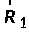
\includegraphics[width=\linewidth,height=.72\textheight,keepaspectratio]{images/image33.pdf}\textbf{=}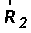
\includegraphics[width=\linewidth,height=.72\textheight,keepaspectratio]{images/image34.pdf}
\item
  Exprimés au \textbf{même point}, leurs moments sont égaux $\rightarrow$
  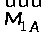
\includegraphics[width=\linewidth,height=.72\textheight,keepaspectratio]{images/image35.pdf}\textbf{=}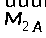
\includegraphics[width=\linewidth,height=.72\textheight,keepaspectratio]{images/image36.pdf}
\end{itemize}

\(\left\{ T1 \right\} = \left\{ \left. \ \begin{matrix}
X_{1} \\
Y_{1} \\
Z_{1}
\end{matrix} \right|\begin{matrix}
L_{1} \\
M_{1} \\
N_{1}
\end{matrix} \right\}_{\text{A,}\overrightarrow{\text{i}}\text{,}\overrightarrow{\text{j}}\text{,}\overrightarrow{\text{k}}}\),
\(\left\{ T2 \right\} = \left\{ \left. \ \begin{matrix}
X_{2} \\
Y_{2} \\
Z_{2}
\end{matrix} \right|\begin{matrix}
L_{2} \\
M_{2} \\
N_{2}
\end{matrix} \right\}_{\text{A,}\overrightarrow{\text{i}}\text{,}\overrightarrow{\text{j}}\text{,}\overrightarrow{\text{k}}}\)
\(\left\{ T1 \right\} = \left\{ T2 \right\}\text{ si }\begin{matrix}
X_{1} = X_{2} \\
Y_{1} = Y_{2} \\
Z_{1} = Z_{2}
\end{matrix}\text{ ET  }\begin{matrix}
L_{1} = L_{2} \\
M_{1} = M_{2} \\
N_{1} = N_{2}
\end{matrix}\)

\textbf{Bien faire attention à bien exprimer les torseurs au même
point~!!}

\subparagraph*{Somme de deux torseurs}\label{somme-de-deux-torseurs}
\addcontentsline{toc}{subparagraph}{Somme de deux torseurs}

La somme de deux torseurs\{ \emph{T} \textsubscript{1}\} et \{ \emph{T}
\textsubscript{2}\} est un torseur tel que :
\(\left\{ T_{1} \right\} + \left\{ T_{2} \right\} = \begin{Bmatrix}
{\overrightarrow{R}}_{1} + {\overrightarrow{R}}_{2} \\
{\overrightarrow{M_{1}}}_{A} + {\overrightarrow{M_{2}}}_{A}
\end{Bmatrix}_{A}\)

\emph{\textbf{On prendra bien soin, d'exprimer les torseurs au même
point avant de les additionner}}

\[\left\{ T_{1} \right\} + \left\{ T_{2} \right\} = \left\{ \left. \ \begin{matrix}
X_{1} + X_{2} \\
Y_{1} + Y_{2} \\
Z_{1} + Z_{2}
\end{matrix} \right|\begin{matrix}
L_{1} + L_{2} \\
M_{1} + M_{2} \\
N_{1} + N_{2}
\end{matrix} \right\}_{\text{A,}\overrightarrow{\text{i}}\text{,}\overrightarrow{\text{j}}\text{,}\overrightarrow{\text{k}}}\]

\subparagraph*{Comoment (Produit) de deux
torseurs}\label{comoment-produit-de-deux-torseurs}
\addcontentsline{toc}{subparagraph}{Comoment (Produit) de deux torseurs}

Très utilisé pour appliquer les théorèmes énergétiques, le comoment de
deux torseurs\{\emph{T}\textsubscript{1}\} et
\{\emph{T}\textsubscript{2}\} est le \textbf{nombre réel} suivant :
\(\left\{ T_{1} \right\} \otimes \left\{ T_{2} \right\} = {\overrightarrow{R}}_{1} \bullet {\overrightarrow{M_{2}}}_{A} + {\overrightarrow{R}}_{2} \bullet {\overrightarrow{M_{1}}}_{A}\)

\emph{\textbf{Le résultat du comoment est un réel~! On prendra bien
soin, d'exprimer les torseurs au même point avant de calculer le
comoment !}}

\textbf{Remarque~:} Le résultat du comoment est indépendant du point
choisi pour exprimer les torseurs !
\(\left\{ T_{1} \right\} \otimes \left\{ T_{2} \right\} = \begin{Bmatrix}
{\overrightarrow{R}}_{1} \\
{\overrightarrow{M_{1}}}_{A}
\end{Bmatrix}_{A} \otimes \begin{Bmatrix}
{\overrightarrow{R}}_{2} \\
{\overrightarrow{M_{2}}}_{A}
\end{Bmatrix}_{A} = \begin{Bmatrix}
{\overrightarrow{R}}_{1} \\
{\overrightarrow{M_{1}}}_{B}
\end{Bmatrix}_{B} \otimes \begin{Bmatrix}
{\overrightarrow{R}}_{2} \\
{\overrightarrow{M_{2}}}_{B}
\end{Bmatrix}_{B}\)

\subsubsection{Mouvements}\label{mouvements}

La connaissance des résultats de cinématique des mouvements particuliers
permet de gagner du temps lors de la détermination des vecteurs vitesse
ou accélération de points appartenant à un solide en mouvement complexe
par rapport à un repère de référence.

Un mouvement est un \emph{\textbf{déplacement relatif d'un solide par
rapport à un autre}}, il met en jeu trois entités~:

\begin{itemize}
\item
  \emph{\textbf{Le solide observé~;}}
\item
  \emph{\textbf{Le solide de référence~;}}
\item
  \emph{\textbf{Le temps.}}
\end{itemize}

\emph{\ul{Notation~}: le mouvement d'un solide S par rapport à un solide
0 est noté S/0.}

Par exemple, il n'est pas forcément facile de voir un coucher de Terre
depuis la Lune~:


\includegraphics[width=\linewidth,height=.72\textheight,keepaspectratio]{images/image37.jpeg}

\subsubsection{Trajectoire}\label{trajectoire}

La trajectoire (\emph{un segment de droite, un arc de cercle ou une
courbe quelconque}) d'un point appartenant à un solide, dans son
mouvement par rapport à un autre solide, est le \emph{\textbf{lieu des
positions successives occupées par ce point}} au cours du temps dans le
repère lié au solide de référence.


\includegraphics[width=\linewidth,height=.72\textheight,keepaspectratio]{images/image38.png}Remarque~:
\emph{N'importe quel point de l'espace peut être considéré comme
appartenant à un solide, y compris un point où il n'y a pas de matière.}

\emph{\textbf{M}}

\emph{Ex~: un point sur l'axe d'un cylindre creux.}

\emph{\textbf{Notation~:} la trajectoire d'un point}
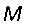
\includegraphics[width=\linewidth,height=.72\textheight,keepaspectratio]{images/image39.pdf}\emph{appartenant à un solide S
dans son mouvement par rapport à un solide 0 est notée}
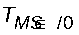
\includegraphics[width=\linewidth,height=.72\textheight,keepaspectratio]{images/image40.pdf}\emph{.}

Dans cet exemple de robot soudeur (Panasonic), la trajectoire
\(T_{M \in S/0}\) correspond exactement au cordon de soudure réalisé par
le robot. Le point 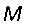
\includegraphics[width=\linewidth,height=.72\textheight,keepaspectratio]{images/image41.pdf} est un point
situé à l'extrémité de la buse de soudage (solide \emph{S}).

Le repère de référence
\(R_{0}(O_{0},\overrightarrow{x_{0}},\overrightarrow{y_{0}},\overrightarrow{z_{0}})\)
est lié au socle du robot (solide 0).

\subsubsection{Mouvements particuliers}\label{mouvements-particuliers}

\paragraph*{}\label{section}
\addcontentsline{toc}{paragraph}{}

\paragraph*{Mouvement de translation}\label{mouvement-de-translation}
\addcontentsline{toc}{paragraph}{Mouvement de translation}

Un solide 2 est en mouvement de translation par rapport à un repère
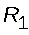
\includegraphics[width=\linewidth,height=.72\textheight,keepaspectratio]{images/image42.pdf} (associé au solide 1), \textbf{si
le vecteur rotation} \(\overrightarrow{\mathbf{\Omega}_{\mathbf{2/1}}}\)
\textbf{est nul}. Lors d'un mouvement de translation d'un solide par
rapport à un repère de référence, un segment qui relie 2 points du
solide reste toujours parallèle à lui-même.

D'après la relation du champ des vecteurs vitesse, cela implique que
\textbf{tous les points du solide ont le même vecteur vitesse}. Donc~:
\(\left\{ V_{2/1} \right\} = \begin{Bmatrix}
\overrightarrow{0} \\
\overrightarrow{V_{P \in 2/1}}
\end{Bmatrix}_{\forall\ P\ \epsilon\ 2}\)

Il existe plusieurs types de mouvement de translation~:

\begin{longtable}{@{}
  >{\raggedright\arraybackslash}p{(\columnwidth - 2\tabcolsep) * \real{0.5000}}
  >{\raggedright\arraybackslash}p{(\columnwidth - 2\tabcolsep) * \real{0.5000}}@{}}
\toprule\noalign{}
\begin{minipage}[b]{\linewidth}\raggedright
Translation rectiligne
\end{minipage} & \begin{minipage}[b]{\linewidth}\raggedright
Translation circulaire
\end{minipage} \\
\midrule\noalign{}
\endhead
\bottomrule\noalign{}
\endlastfoot

\includegraphics[width=\linewidth,height=.72\textheight,keepaspectratio]{images/image43.png}\emph{Les
trajectoires des points sont des segments de droite} & \emph{Les
trajectoires des points sont des arcs de cercle de même rayon}


\includegraphics[width=\linewidth,height=.72\textheight,keepaspectratio]{images/image44.png} \\
\multicolumn{2}{@{}>{\raggedright\arraybackslash}p{(\columnwidth - 2\tabcolsep) * \real{1.0000} + 2\tabcolsep}@{}}{%
translation curviligne} \\
\multicolumn{2}{@{}>{\raggedright\arraybackslash}p{(\columnwidth - 2\tabcolsep) * \real{1.0000} + 2\tabcolsep}@{}}{%
\emph{Les trajectoires des points sont des courbes quelconques}


\includegraphics[width=\linewidth,height=.72\textheight,keepaspectratio]{images/image45.png}} \\
\end{longtable}

\paragraph*{Mouvement de rotation}\label{mouvement-de-rotation}
\addcontentsline{toc}{paragraph}{Mouvement de rotation}

Un solide 2 est en mouvement de rotation autour d'un axe
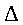
\includegraphics[width=\linewidth,height=.72\textheight,keepaspectratio]{images/image46.pdf} par rapport à un repère
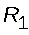
\includegraphics[width=\linewidth,height=.72\textheight,keepaspectratio]{images/image42.pdf} (associé au solide 1), si en tout
point 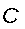
\includegraphics[width=\linewidth,height=.72\textheight,keepaspectratio]{images/image47.pdf} de l'axe
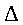
\includegraphics[width=\linewidth,height=.72\textheight,keepaspectratio]{images/image46.pdf}~:
\(\left\{ V_{2/1} \right\} = \begin{Bmatrix}
\overrightarrow{\Omega_{2/1}} \\
\overrightarrow{0}
\end{Bmatrix}_{\forall\ C\ \epsilon\ \mathrm{\Delta}}\)

\begin{itemize}
\item
  
\includegraphics[width=\linewidth,height=.72\textheight,keepaspectratio]{images/image48.png}Pour
  tout point \(C \in \Delta\), on a
  \(\overrightarrow{V_{C \in 2/1}} = \overrightarrow{0}\)\textsuperscript{~};
\item
  \(\overrightarrow{\Omega_{2/1}}\) est colinéaire à \(\Delta\), appelé
  axe de rotation ;
\item
  Tous les points du solide 2 ont, dans leur mouvement par rapport au
  solide 1 une \textbf{trajectoire en forme d'arc de cercle}~;
\item
  \textbf{Le vecteur vitesse}
  \(\overrightarrow{\mathbf{V}_{\mathbf{M}_{\mathbf{i}}\mathbf{\in}\mathbf{2/1}}}\)
  de tout point \(M_{i} \notin \Delta\)du solide 2 \textbf{est tangent à
  sa trajectoire en arc de cercle et a une norme proportionnelle à la
  distance qui sépare le point} \(\mathbf{M}_{\mathbf{i}}\)\textbf{de
  l'axe} \(\mathbf{\Delta}\)\textbf{.}
\end{itemize}

En effet, si \(C\) est le projeté orthogonal de \(M\) sur \(\Delta\), on
a~:

\[\overrightarrow{V_{M \in 2/1}} = \underset{\overrightarrow{0}}{\overset{\overrightarrow{V_{C \in 2/1}}}{}} + \overrightarrow{MC} \land \overrightarrow{\Omega_{2/1}} = \overrightarrow{MC} \land \overrightarrow{\Omega_{2/1}}\]

\textbf{Remarque}~: c'est la version vectorielle de la relation
\(V = \omega \times R\)\ldots.

\paragraph*{Mouvement quelconque}\label{mouvement-quelconque}
\addcontentsline{toc}{paragraph}{Mouvement quelconque}

Lorsqu'un solide a un mouvement relatif qui n'est ni une translation ni
une rotation, alors on dit qu'il a un mouvement quelconque (ou plan).

\begin{longtable}{@{}
  >{\raggedright\arraybackslash}p{(\columnwidth - 2\tabcolsep) * \real{0.1227}}
  >{\raggedright\arraybackslash}p{(\columnwidth - 2\tabcolsep) * \real{0.8773}}@{}}
\toprule\noalign{}
\begin{minipage}[b]{\linewidth}\raggedright
\begin{quote}

\includegraphics[width=\linewidth,height=.72\textheight,keepaspectratio]{images/image18.png}
\end{quote}
\end{minipage} & \begin{minipage}[b]{\linewidth}\raggedright
\textbf{Machine 5 axes}

\(\overrightarrow{O_{0}O_{4}} = x(t) \cdot \overrightarrow{x_{0}} + d \cdot \overrightarrow{z_{0}}\)

\[\overrightarrow{AO_{1}} = a \cdot \overrightarrow{z_{1}}\]

\[\overrightarrow{\mathbf{O}_{\mathbf{4}}\mathbf{D}}\mathbf{= e}\mathbf{\cdot}\overrightarrow{\mathbf{y}_{\mathbf{4}}}\mathbf{\ \ \ \ \ \ \ \ \ \ \ \ \ \ \ \ \ \ \ \ \ \ \ \ \ \ \ \ }\]

\(\mathbf{\ }\overrightarrow{O_{0}A} = y(t) \cdot \overrightarrow{y_{0}}\)
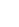
\includegraphics[width=\linewidth,height=.72\textheight,keepaspectratio]{images/image27.pdf}

\(\overrightarrow{O_{1}O_{2}} = b \cdot \overrightarrow{x_{2}}\)

\[\overrightarrow{\mathbf{O}_{\mathbf{5}}\mathbf{P}}\mathbf{=}\mathbf{-}\mathbf{f}\mathbf{\cdot}\overrightarrow{\mathbf{z}_{\mathbf{5}}}\]

\(\overrightarrow{DO_{5}} = - z(t) \cdot \overrightarrow{z_{4}}\)

\(\overrightarrow{O_{2}O_{3}} = c \cdot \overrightarrow{z_{3}}\)

\(\mathbf{\alpha =}\left( \overrightarrow{\mathbf{y}_{\mathbf{1}}}\mathbf{,}\overrightarrow{\mathbf{y}_{\mathbf{2}}} \right)\)
et
\(\beta = \left( \overrightarrow{x_{2}},\overrightarrow{x_{3}} \right)\)


\includegraphics[width=\linewidth,height=.72\textheight,keepaspectratio]{images/image49.png}

\begin{enumerate}
\def\labelenumi{\arabic{enumi}.}
\item
  Indiquer la nature du mouvement du solide 1 par rapport au solide 0.
\end{enumerate}

\textbf{Mouvement de translation rectiligne}
\(\overrightarrow{\mathbf{\Omega}_{\mathbf{1/0}}}\mathbf{=}\overrightarrow{\mathbf{0}}\)

\begin{enumerate}
\def\labelenumi{\arabic{enumi}.}
\setcounter{enumi}{1}
\item
  Indiquer la nature du mouvement du solide 4 par rapport au solide 0.
\end{enumerate}

\textbf{Mouvement de translation rectiligne}
\(\overrightarrow{\mathbf{\Omega}_{\mathbf{4}\mathbf{/0}}}\mathbf{=}\overrightarrow{\mathbf{0}}\)

\begin{enumerate}
\def\labelenumi{\arabic{enumi}.}
\setcounter{enumi}{2}
\item
  Indiquer la nature du mouvement du solide 5 par rapport au solide 4.
\end{enumerate}

\textbf{Mouvement de translation rectiligne}
\(\overrightarrow{\mathbf{\Omega}_{\mathbf{5}\mathbf{/}\mathbf{4}}}\mathbf{=}\overrightarrow{\mathbf{0}}\)

\begin{enumerate}
\def\labelenumi{\arabic{enumi}.}
\setcounter{enumi}{3}
\item
  En déduire la relation entre les bases
  \(B_{0},B_{1}, B_{4}\ et\ B_{5}\) .
\end{enumerate}

\[B_{0} = B_{1} = B_{4} = B_{5}\]

\begin{enumerate}
\def\labelenumi{\arabic{enumi}.}
\setcounter{enumi}{4}
\item
  Indiquer la nature du mouvement du solide 2 par rapport au solide 1.
\end{enumerate}

\textbf{Mouvement de rotation d'axe}
\(\overrightarrow{\mathbf{x}_{\mathbf{2}}}\)

\begin{enumerate}
\def\labelenumi{\arabic{enumi}.}
\setcounter{enumi}{5}
\item
  Dessiner la figure de changement de base correspondant à ce mouvement.
\end{enumerate}

\[\overrightarrow{\mathbf{y}_{\mathbf{1}}}\]

\[\overrightarrow{\mathbf{y}_{\mathbf{2}}}\]

\[\overrightarrow{\mathbf{z}_{\mathbf{1}}}\]

\[\overrightarrow{\mathbf{z}_{\mathbf{2}}}\]

\[\overrightarrow{\mathbf{x}_{\mathbf{1}}}\mathbf{=}\overrightarrow{\mathbf{x}_{\mathbf{2}}}\]

\[\alpha\]

\(\mathbf{\alpha}\)

\begin{enumerate}
\def\labelenumi{\arabic{enumi}.}
\setcounter{enumi}{6}
\item
  Indiquer la nature du mouvement du solide 3 par rapport au solide 2.
\end{enumerate}

\textbf{Mouvement de rotation d'axe}
\(\overrightarrow{\mathbf{z}_{\mathbf{2}}}\)

\begin{enumerate}
\def\labelenumi{\arabic{enumi}.}
\setcounter{enumi}{7}
\item
  Dessiner la figure de changement de base correspondant à ce mouvement.
\end{enumerate}

\[\overrightarrow{\mathbf{x}_{\mathbf{2}}}\]

\[\overrightarrow{\mathbf{x}_{\mathbf{3}}}\]

\[\overrightarrow{\mathbf{y}_{\mathbf{2}}}\]

\[\overrightarrow{\mathbf{y}_{\mathbf{3}}}\]

\[\overrightarrow{\mathbf{z}_{\mathbf{2}}}\mathbf{=}\overrightarrow{\mathbf{z}_{\mathbf{3}}}\]

\[\beta\]

\(\mathbf{\beta}\)

\begin{enumerate}
\def\labelenumi{\arabic{enumi}.}
\setcounter{enumi}{8}
\item
  Déterminer le vecteur rotation \(\overrightarrow{\Omega_{3/2}}\).
\end{enumerate}

\textbf{Voir paragraphe suivant~:D}

\begin{enumerate}
\def\labelenumi{\arabic{enumi}.}
\setcounter{enumi}{9}
\item
  En déduire le vecteur rotation \(\overrightarrow{\Omega_{3/0}}\).
\end{enumerate}

\textbf{Voir paragraphe suivant~:D}
\end{minipage} \\
\midrule\noalign{}
\endhead
\bottomrule\noalign{}
\endlastfoot
& \\
\end{longtable}

\subsubsection{Vecteur rotation}\label{vecteur-rotation}

Le vecteur rotation, noté \(\overrightarrow{\Omega_{i/j}}\)caractérise~:

\begin{itemize}
\item
  par sa \emph{\textbf{direction}}, la direction de l'axe autour duquel
  la base du repère \(R_{i}\) tourne autour de la base du repère
  \(R_{j}\)~;
\item
  par sa \emph{\textbf{norme}} (\emph{exprimée en}
  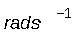
\includegraphics[width=\linewidth,height=.72\textheight,keepaspectratio]{images/image50.pdf}), la vitesse de ce mouvement de
  rotation relatif~;
\item
  par son \emph{\textbf{signe (}un signe positif correspond à un sens de
  rotation qui conduit à un vecteur positif par la règle du
  «~tire-bouchon~».}\textbf{)}, le sens de ce mouvement de rotation
  relatif.
\end{itemize}


\includegraphics[width=\linewidth,height=.72\textheight,keepaspectratio]{images/image51.png}\emph{\textbf{Exemple~:}
bras manipulateur}

Pour déterminer un vecteur vitesse rotation, la composition des vitesses
peut être utilisées (elle sera vue plus tard dans ces cours de manière
plus générique)~:

\[\overrightarrow{\Omega_{3/0}} = \overrightarrow{\Omega_{3/2}} + \overrightarrow{\Omega_{2/1}} + \overrightarrow{\Omega_{1/0}}\]

\begin{longtable}{@{}
  >{\raggedright\arraybackslash}p{(\columnwidth - 2\tabcolsep) * \real{0.1227}}
  >{\raggedright\arraybackslash}p{(\columnwidth - 2\tabcolsep) * \real{0.8773}}@{}}
\toprule\noalign{}
\begin{minipage}[b]{\linewidth}\raggedright
\begin{quote}

\includegraphics[width=\linewidth,height=.72\textheight,keepaspectratio]{images/image18.png}
\end{quote}
\end{minipage} & \begin{minipage}[b]{\linewidth}\raggedright
\textbf{Machine 5 axes}

\begin{enumerate}
\def\labelenumi{\arabic{enumi}.}
\item
  Déterminer le vecteur rotation \(\overrightarrow{\Omega_{3/2}}\).
\end{enumerate}

\[\overrightarrow{\Omega_{3/2}} = \dot{\beta}\ \overrightarrow{z_{2}} = \dot{\beta}\ \overrightarrow{z_{3}}\]

\begin{enumerate}
\def\labelenumi{\arabic{enumi}.}
\setcounter{enumi}{1}
\item
  En déduire le vecteur rotation \(\overrightarrow{\Omega_{3/0}}\).
\end{enumerate}

\[\overrightarrow{\mathbf{\Omega}_{\mathbf{3/0}}}\mathbf{=}\overrightarrow{\mathbf{\Omega}_{\mathbf{3/2}}}\mathbf{+}\overrightarrow{\mathbf{\Omega}_{\mathbf{2/1}}}\mathbf{+}\overrightarrow{\mathbf{\Omega}_{\mathbf{1/0}}}\]

\textbf{Or}
\(\overrightarrow{\mathbf{\Omega}_{\mathbf{1/0}}}\mathbf{=}\overrightarrow{\mathbf{0}}\)
\textbf{translation et}
\(\overrightarrow{\mathbf{\Omega}_{\mathbf{2/1}}}\mathbf{=}\dot{\mathbf{\alpha}}\mathbf{\ }\overrightarrow{\mathbf{x}_{\mathbf{2}}}\)

\[\overrightarrow{\mathbf{\Omega}_{\mathbf{3/0}}}\mathbf{=}\dot{\mathbf{\beta}}\mathbf{\ }\overrightarrow{\mathbf{z}_{\mathbf{2}}}\mathbf{+}\dot{\mathbf{\alpha}}\mathbf{\ }\overrightarrow{\mathbf{x}_{\mathbf{2}}}\]
\end{minipage} \\
\midrule\noalign{}
\endhead
\bottomrule\noalign{}
\endlastfoot
& \\
\end{longtable}

\subsubsection[Vecteur
position]{\texorpdfstring{\protect
\includegraphics[width=\linewidth,height=.72\textheight,keepaspectratio]{images/image52.png}Vecteur
position}{Vecteur position}}\label{vecteur-position}

Le vecteur position d'un point
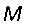
\includegraphics[width=\linewidth,height=.72\textheight,keepaspectratio]{images/image53.pdf}appartenant à un solide
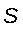
\includegraphics[width=\linewidth,height=.72\textheight,keepaspectratio]{images/image54.pdf} est le vecteur qui lie ce point
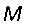
\includegraphics[width=\linewidth,height=.72\textheight,keepaspectratio]{images/image53.pdf} à l'origine
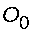
\includegraphics[width=\linewidth,height=.72\textheight,keepaspectratio]{images/image55.pdf} du repère de référence
\(R_{0}(O_{0},\overrightarrow{x_{0}},\overrightarrow{y_{0}},\overrightarrow{z_{0}})\).

A la date \emph{t~}:
\(\overrightarrow{O_{0}M} = a(t) \cdot \overrightarrow{x} + b(t) \cdot \overrightarrow{y} + c(t) \cdot \overrightarrow{z}\)

\textbf{Remarque~:} \emph{Pour alléger les notations dans la suite, on
n'écrira plus la variable \textbf{t}. Cependant, il faudra bien garder à
l'esprit que les coordonnées du vecteur position varient au cours du
temps.}

Selon le mouvement relatif étudié, il peut être judicieux d'exprimer le
vecteur position à l'aide des coordonnées autres que les
\emph{\textbf{coordonnées cartésiennes}}~:

\begin{longtable}{@{}
  >{\raggedright\arraybackslash}p{(\columnwidth - 2\tabcolsep) * \real{0.5002}}
  >{\raggedright\arraybackslash}p{(\columnwidth - 2\tabcolsep) * \real{0.4998}}@{}}
\toprule\noalign{}
\begin{minipage}[b]{\linewidth}\raggedright
\emph{\textbf{Coordonnées cylindriques}}
\end{minipage} & \begin{minipage}[b]{\linewidth}\raggedright
\emph{\textbf{Coordonnées sphériques}}
\end{minipage} \\
\midrule\noalign{}
\endhead
\bottomrule\noalign{}
\endlastfoot
\emph{r, $\theta$ et z} & \emph{r, $\theta$ et $\varphi$} \\

\includegraphics[width=\linewidth,height=.72\textheight,keepaspectratio]{images/image56.png}
&

\includegraphics[width=\linewidth,height=.72\textheight,keepaspectratio]{images/image57.png} \\
\(\overrightarrow{OM} = r \cdot \overrightarrow{u} + z \cdot \overrightarrow{z}\)

avec
\(\overrightarrow{u} = \cos\theta \cdot \overrightarrow{x} + \sin\theta \cdot \overrightarrow{y}\)
& \(\overrightarrow{OM} = r \cdot \overrightarrow{n}\)

avec
\(\overrightarrow{n} = \cos\phi \cdot \overrightarrow{z} + \sin\phi \cdot \overrightarrow{u}\) \\
\emph{\textbf{\ul{Exemple~:}} Vecteur position d'un point M appartenant
à un portail en mouvement par rapport au sol.}


\includegraphics[width=\linewidth,height=.72\textheight,keepaspectratio]{images/image58.jpeg}
& \begin{minipage}[t]{\linewidth}\raggedright
\begin{quote}
\emph{\textbf{\ul{Exemple~:}} Vecteur position d'un point M appartenant
à un radar de poursuite en mouvement par rapport à la coque d'un navire
de guerre.}


\includegraphics[width=\linewidth,height=.72\textheight,keepaspectratio]{images/image59.jpeg}
\end{quote}
\end{minipage} \\
\end{longtable}

\begin{longtable}{@{}
  >{\raggedright\arraybackslash}p{(\columnwidth - 2\tabcolsep) * \real{0.1227}}
  >{\raggedright\arraybackslash}p{(\columnwidth - 2\tabcolsep) * \real{0.8773}}@{}}
\toprule\noalign{}
\begin{minipage}[b]{\linewidth}\raggedright
\begin{quote}

\includegraphics[width=\linewidth,height=.72\textheight,keepaspectratio]{images/image18.png}
\end{quote}
\end{minipage} & \begin{minipage}[b]{\linewidth}\raggedright
\textbf{Machine 5 axes}

\(\overrightarrow{O_{0}O_{4}} = x(t) \cdot \overrightarrow{x_{0}} + d \cdot \overrightarrow{z_{0}}\)

\[\overrightarrow{AO_{1}} = a \cdot \overrightarrow{z_{1}}\]

\[\overrightarrow{O_{4}D} = e \cdot \overrightarrow{y_{4}}\ \ \ \ \ \ \ \ \ \ \ \ \ \ \ \ \ \ \ \ \ \ \ \ \ \ \ \ \]

\(\mathbf{\ }\overrightarrow{O_{0}A} = y(t) \cdot \overrightarrow{y_{0}}\)
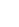
\includegraphics[width=\linewidth,height=.72\textheight,keepaspectratio]{images/image27.pdf}

\(\overrightarrow{O_{1}O_{2}} = b \cdot \overrightarrow{x_{2}}\)

\[\overrightarrow{O_{5}P} = - f \cdot \overrightarrow{z_{5}}\]

\(\overrightarrow{DO_{5}} = - z(t) \cdot \overrightarrow{z_{4}}\)

\(\overrightarrow{O_{2}O_{3}} = c \cdot \overrightarrow{z_{3}}\)

\(\alpha = \left( \overrightarrow{y_{1}},\overrightarrow{y_{2}} \right)\)
et
\(\beta = \left( \overrightarrow{x_{2}},\overrightarrow{x_{3}} \right)\)


\includegraphics[width=\linewidth,height=.72\textheight,keepaspectratio]{images/image49.png}

\begin{enumerate}
\def\labelenumi{\arabic{enumi}.}
\item
  Exprimer le vecteur position \(\overrightarrow{O_{0}P}\) dans la base
  du référentiel \(R_{0}\).
\end{enumerate}

\[\overrightarrow{\mathbf{O}_{\mathbf{0}}\mathbf{P}}\mathbf{=}\overrightarrow{\mathbf{O}_{\mathbf{0}}\mathbf{O}_{\mathbf{4}}}\mathbf{+}\overrightarrow{\mathbf{O}_{\mathbf{4}}\mathbf{D}}\mathbf{+}\overrightarrow{\mathbf{D}\mathbf{O}_{\mathbf{5}}}\mathbf{+}\overrightarrow{\mathbf{O}_{\mathbf{5}}\mathbf{P}}\]

\[\overrightarrow{\mathbf{O}_{\mathbf{0}}\mathbf{P}}\mathbf{=}\mathbf{x}\left( \mathbf{t} \right)\overrightarrow{\mathbf{x}_{\mathbf{0}}}\mathbf{+ d}\overrightarrow{\mathbf{z}_{\mathbf{0}}}\mathbf{+}\mathbf{e}\overrightarrow{\mathbf{y}_{\mathbf{4}}}\mathbf{- z}\left( \mathbf{t} \right)\overrightarrow{\mathbf{z}_{\mathbf{4}}}\mathbf{- f}\overrightarrow{\mathbf{z}_{\mathbf{5}}}\]

\textbf{Or}
\(\mathbf{B}_{\mathbf{0}}\mathbf{=}\mathbf{B}_{\mathbf{1}}\mathbf{=}\mathbf{}\mathbf{B}_{\mathbf{4}}\mathbf{=}\mathbf{B}_{\mathbf{5}}\)
\textbf{donc}

\[\overrightarrow{\mathbf{O}_{\mathbf{0}}\mathbf{P}}\mathbf{=}\mathbf{x}\left( \mathbf{t} \right)\overrightarrow{\mathbf{x}_{\mathbf{0}}}\mathbf{+ d}\overrightarrow{\mathbf{z}_{\mathbf{0}}}\mathbf{+}\mathbf{e}\overrightarrow{\mathbf{y}_{\mathbf{0}}}\mathbf{- z}\left( \mathbf{t} \right)\overrightarrow{\mathbf{z}_{\mathbf{0}}}\mathbf{- f}\overrightarrow{\mathbf{z}_{\mathbf{0}}}\]

\begin{enumerate}
\def\labelenumi{\arabic{enumi}.}
\setcounter{enumi}{1}
\item
  Exprimer le vecteur position \(\overrightarrow{O_{0}O_{3}}\) dans les
  bases des référentiels \(R_{0}\) et \(R_{2}\)
\end{enumerate}

\[\overrightarrow{\mathbf{O}_{\mathbf{0}}\mathbf{O}_{\mathbf{3}}}\mathbf{=}\overrightarrow{\mathbf{O}_{\mathbf{0}}\mathbf{A}}\mathbf{+}\overrightarrow{{\mathbf{A}\mathbf{O}}_{\mathbf{1}}}\mathbf{+}\overrightarrow{\mathbf{O}_{\mathbf{1}}\mathbf{O}_{\mathbf{2}}}\mathbf{+}\overrightarrow{\mathbf{O}_{\mathbf{2}}\mathbf{O}_{\mathbf{3}}}\]

\[\overrightarrow{\mathbf{O}_{\mathbf{0}}\mathbf{O}_{\mathbf{3}}}\mathbf{=}\mathbf{y}\left( \mathbf{t} \right)\overrightarrow{\mathbf{y}_{\mathbf{0}}}\mathbf{+}\mathbf{a}\overrightarrow{\mathbf{z}_{\mathbf{1}}}\mathbf{+}\mathbf{b}\overrightarrow{\mathbf{x}_{\mathbf{2}}}\mathbf{+}\mathbf{\ }\mathbf{c}\overrightarrow{\mathbf{z}_{\mathbf{3}}}\]

\[\overrightarrow{\mathbf{O}_{\mathbf{0}}\mathbf{O}_{\mathbf{3}}}\mathbf{=}\mathbf{y}\left( \mathbf{t} \right)\overrightarrow{\mathbf{y}_{\mathbf{0}}}\mathbf{+}\mathbf{a}\overrightarrow{\mathbf{z}_{\mathbf{0}}}\mathbf{+}\mathbf{b}\overrightarrow{\mathbf{x}_{\mathbf{0}}}\mathbf{+}\mathbf{\ }\mathbf{c}\overrightarrow{\mathbf{z}_{\mathbf{2}}}\]

\begin{enumerate}
\def\labelenumi{\arabic{enumi}.}
\setcounter{enumi}{2}
\item
  Déterminer le vecteur vitesse \(\overrightarrow{V_{P \in 5/0}}\ \)du
  point \(P\) appartenant à l'outil, dans son mouvement par rapport
  à~\(R_{0}\).
\end{enumerate}

\textbf{Voir paragraphe suivant~pour savoir comment faire :D.}
\end{minipage} \\
\midrule\noalign{}
\endhead
\bottomrule\noalign{}
\endlastfoot
\end{longtable}

\subsubsection[Vecteur
vitesse]{\texorpdfstring{\protect
\includegraphics[width=\linewidth,height=.72\textheight,keepaspectratio]{images/image3.png}Vecteur
vitesse}{Vecteur vitesse}}\label{vecteur-vitesse}

Le vecteur vitesse est la \emph{\textbf{dérivée}}, par rapport au temps,
\emph{\textbf{du vecteur position}} dans un repère de référence.
\emph{Ce vecteur est \textbf{\ul{tangent à la trajectoire}}}
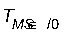
\includegraphics[width=\linewidth,height=.72\textheight,keepaspectratio]{images/image60.pdf}. \emph{Sa norme est exprimée en}
\(m \cdot s^{- 1}\).

Le vecteur vitesse du point
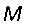
\includegraphics[width=\linewidth,height=.72\textheight,keepaspectratio]{images/image53.pdf}appartenant au solide S dans son
mouvement par rapport à
\(R_{0}(O_{0},\overrightarrow{x_{0}},\overrightarrow{y_{0}},\overrightarrow{z_{0}})\)
est~:

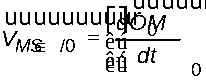
\includegraphics[width=\linewidth,height=.72\textheight,keepaspectratio]{images/image61.pdf} ou
\(\overrightarrow{V_{M \in S/0}} = \left\lbrack \frac{d\overrightarrow{QM}}{dt} \right\rbrack_{0}\)
\emph{si Q est un point fixe
dans}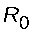
\includegraphics[width=\linewidth,height=.72\textheight,keepaspectratio]{images/image62.pdf}\emph{qui est le repère de
dérivation.}

\emph{\ul{Remarque~:}}
\(\boxed{\overrightarrow{V_{M \in 1/0}} = - \overrightarrow{V_{M \in 0/1}}}\)

\subsubsection{Vecteur accélération}\label{vecteur-accuxe9luxe9ration}

Le vecteur accélération~est la \emph{\textbf{dérivée}}, par rapport au
temps, \emph{\textbf{du vecteur vitesse}} dans le repère de référence.
\emph{Sa norme est exprimée en} 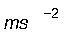
\includegraphics[width=\linewidth,height=.72\textheight,keepaspectratio]{images/image63.pdf}.

Le vecteur accélération du point
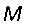
\includegraphics[width=\linewidth,height=.72\textheight,keepaspectratio]{images/image53.pdf}appartenant au solide S dans son
mouvement par rapport à 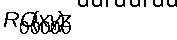
\includegraphics[width=\linewidth,height=.72\textheight,keepaspectratio]{images/image64.pdf} est~:

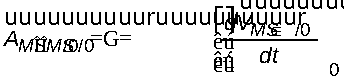
\includegraphics[width=\linewidth,height=.72\textheight,keepaspectratio]{images/image65.pdf}

\begin{longtable}{@{}
  >{\raggedright\arraybackslash}p{(\columnwidth - 2\tabcolsep) * \real{0.1227}}
  >{\raggedright\arraybackslash}p{(\columnwidth - 2\tabcolsep) * \real{0.8773}}@{}}
\toprule\noalign{}
\begin{minipage}[b]{\linewidth}\raggedright
\begin{quote}

\includegraphics[width=\linewidth,height=.72\textheight,keepaspectratio]{images/image18.png}
\end{quote}
\end{minipage} & \begin{minipage}[b]{\linewidth}\raggedright
\textbf{Machine 5 axes}

\begin{enumerate}
\def\labelenumi{\arabic{enumi}.}
\item
  Donner le vecteur position permettant de déterminer la vitesse
  \(\overrightarrow{V_{D \in 4/0}}\).
\end{enumerate}

\[\overrightarrow{\mathbf{V}_{\mathbf{D}\mathbf{\in}\mathbf{4/0}}}\mathbf{=}\left. \ \frac{\mathbf{d}\overrightarrow{\mathbf{O}_{\mathbf{0}}\mathbf{D}}}{\mathbf{dt}} \right|_{\mathbf{0}}\]

\begin{enumerate}
\def\labelenumi{\arabic{enumi}.}
\setcounter{enumi}{1}
\item
  Donner le vecteur position permettant de déterminer la vitesse
  \(\overrightarrow{V_{O_{3} \in 3/1}}\).
\end{enumerate}

\[\overrightarrow{\mathbf{V}_{\mathbf{O}_{\mathbf{3}}\mathbf{\in}\mathbf{3}\mathbf{/}\mathbf{1}}}\mathbf{=}\left. \ \frac{\mathbf{d}\overrightarrow{\mathbf{O}_{\mathbf{1}}\mathbf{O}_{\mathbf{3}}}}{\mathbf{dt}} \right|_{\mathbf{1}}\]

\begin{enumerate}
\def\labelenumi{\arabic{enumi}.}
\setcounter{enumi}{2}
\item
  Déterminer le vecteur vitesse : \(\overrightarrow{V_{P \in 5/0}}\) du
  point \(P\) appartenant à l'outil, dans son mouvement par rapport
  à~\(R_{0}\). Cette vitesse sera notée~
\end{enumerate}

\(\overrightarrow{\mathbf{V}_{\mathbf{P}\mathbf{\in}\mathbf{5/0}}}\mathbf{=}\left. \ \frac{\mathbf{d}\overrightarrow{\mathbf{O}_{\mathbf{0}}\mathbf{P}}}{\mathbf{dt}} \right|_{\mathbf{0}}\)

\[\overrightarrow{\mathbf{V}_{\mathbf{P}\mathbf{\in}\mathbf{5/0}}}\mathbf{=}\left. \ \frac{\mathbf{d}\mathbf{(}\mathbf{x}\left( \mathbf{t} \right)\overrightarrow{\mathbf{x}_{\mathbf{0}}}\mathbf{+ d}\overrightarrow{\mathbf{z}_{\mathbf{0}}}\mathbf{+}\mathbf{e}\overrightarrow{\mathbf{y}_{\mathbf{0}}}\mathbf{- z}\left( \mathbf{t} \right)\overrightarrow{\mathbf{z}_{\mathbf{0}}}\mathbf{- f}\overrightarrow{\mathbf{z}_{\mathbf{0}}}\mathbf{)}}{\mathbf{dt}} \right|_{\mathbf{0}}\]

\[\overrightarrow{\mathbf{V}_{\mathbf{P}\mathbf{\in}\mathbf{5/0}}}\mathbf{=}\dot{\mathbf{x}}\overrightarrow{\mathbf{x}_{\mathbf{0}}}\mathbf{-}\dot{\mathbf{z}}\overrightarrow{\mathbf{z}_{\mathbf{0}}}\]

\begin{enumerate}
\def\labelenumi{\arabic{enumi}.}
\setcounter{enumi}{3}
\item
  En déduire la vitesse maximale du point \(P\) appartenant à l'outil,
  dans son mouvement par rapport à~\(R_{0}\).
\end{enumerate}

\textbf{La valeur de la vitesse est obtenue grâce à la norme. Pour la
vitesse maximale, il suffit de remplacer avec les valeurs maximales.}

\[\left\| \overrightarrow{\mathbf{V}_{\mathbf{P}\mathbf{\in}\mathbf{5/0}}} \right\|\mathbf{=}\sqrt{{\dot{\mathbf{x}}}^{\mathbf{2}}\mathbf{+}{\dot{\mathbf{z}}}^{\mathbf{2}}}\]

\begin{enumerate}
\def\labelenumi{\arabic{enumi}.}
\setcounter{enumi}{4}
\item
  Déterminer le vecteur vitesse \(\overrightarrow{V_{O_{3} \in 3/0}}\)
  du point \(O_{3}\) appartenant au solide 3 (pièce usinée + support),
  dans son mouvement par rapport à~\(R_{0}\).
\end{enumerate}

\[\overrightarrow{\mathbf{V}_{\mathbf{O}_{\mathbf{3}}\mathbf{\in}\mathbf{3/0}}}\mathbf{=}\left. \ \frac{\mathbf{d}\mathbf{(}\mathbf{y}\left( \mathbf{t} \right)\overrightarrow{\mathbf{y}_{\mathbf{0}}}\mathbf{+}\mathbf{a}\overrightarrow{\mathbf{z}_{\mathbf{0}}}\mathbf{+}\mathbf{b}\overrightarrow{\mathbf{x}_{\mathbf{0}}}\mathbf{+}\mathbf{\ }\mathbf{c}\overrightarrow{\mathbf{z}_{\mathbf{2}}}\mathbf{)}}{\mathbf{dt}} \right|_{\mathbf{0}}\]

\[\overrightarrow{\mathbf{V}_{\mathbf{O}_{\mathbf{3}}\mathbf{\in}\mathbf{3/0}}}\mathbf{=}\dot{\mathbf{y}}\overrightarrow{\mathbf{y}_{\mathbf{0}}}\mathbf{+ c}\left. \ \frac{\mathbf{d}\mathbf{\ }\overrightarrow{\mathbf{z}_{\mathbf{2}}}}{\mathbf{dt}} \right|_{\mathbf{0}}\]

\textbf{On est bloqués\ldots. Voir paragraphe suivant 3..\ldots.}

\[\left. \ \frac{\mathbf{d}\mathbf{\ }\overrightarrow{\mathbf{z}_{\mathbf{2}}}}{\mathbf{dt}} \right|_{\mathbf{0}}\mathbf{=}\mathbf{\ }\mathbf{??????}\]
\end{minipage} \\
\midrule\noalign{}
\endhead
\bottomrule\noalign{}
\endlastfoot
\end{longtable}

\subsection{DERIVATION VECTORIELLE ET PRODUIT
VECTORIEL}\label{derivation-vectorielle-et-produit-vectoriel}

Lorsque l'on étudie le comportement cinématique des systèmes, on est
souvent amené à déterminer la \emph{\textbf{dérivée}}, par rapport au
temps, d'un \emph{\textbf{vecteur}} dans un repère de référence.

Il s'agit en général d'un vecteur dont on connaît les coordonnés dans
une base
\((\overrightarrow{x_{i}},\overrightarrow{y_{i}},\overrightarrow{z_{i}})\)
en mouvement par rapport à la
base\((\overrightarrow{x_{j}},\overrightarrow{y_{j}},\overrightarrow{z_{j}})\)
du repère de référence \(R_{j}\).


\includegraphics[width=\linewidth,height=.72\textheight,keepaspectratio]{images/image66.png}

\emph{\textbf{Exemple~:} bras manipulateur}

Pour ne pas s'engager dans des calculs longs et fastidieux, on
n'exprimera jamais le vecteur dans la base du repère de référence pour
ensuite dériver ses coordonnées.

\emph{\textbf{On préférera utiliser la formule de la dérivation
vectorielle.}}

\subsubsection{Formule de la dérivation
vectorielle}\label{formule-de-la-duxe9rivation-vectorielle}

On peut déterminer la dérivée, par rapport au temps, d'un vecteur
\(\overrightarrow{U}\) dans un repère de référence
\(R_{j}(O_{j},\overrightarrow{x_{j}},\overrightarrow{y_{j}},\overrightarrow{z_{j}})\),
et dont on connait les coordonnées dans une base
\((\overrightarrow{x_{i}},\overrightarrow{y_{i}},\overrightarrow{z_{i}})\).

Pour cela, on utilise la formule de changement de base ou
\emph{\textbf{formule de Boor}}~:

\[\left\lbrack \frac{d\overrightarrow{U}}{dt} \right\rbrack_{R_{j}} = \left\lbrack \frac{d\overrightarrow{U}}{dt} \right\rbrack_{R_{i}} + \overrightarrow{\Omega_{i/j}} \land \overrightarrow{U}\]

\begin{quote}
\emph{\textbf{\ul{Cas particulier d'un vecteur unitaire~:}}}

Si \(\overrightarrow{U}\) est un vecteur unitaire de la base du repère
\(R_{i}\) (\(\overrightarrow{x_{i}}\) par exemple), on a alors~:
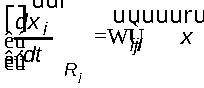
\includegraphics[width=\linewidth,height=.72\textheight,keepaspectratio]{images/image67.pdf} \emph{car}
\(\overrightarrow{x_{i}}\) \emph{est fixe dans la base du repère}
\(R_{i}\) \emph{est le repère de dérivation.}
\end{quote}


\includegraphics[width=\linewidth,height=.72\textheight,keepaspectratio]{images/image68.png}\emph{\ul{\textbf{Exemple~}:
bras manipulateur}}

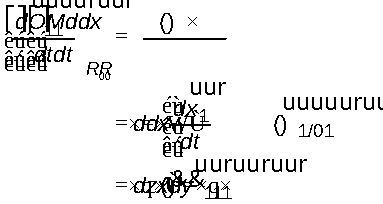
\includegraphics[width=\linewidth,height=.72\textheight,keepaspectratio]{images/image69.pdf}

\begin{longtable}{@{}
  >{\raggedright\arraybackslash}p{(\columnwidth - 2\tabcolsep) * \real{0.1227}}
  >{\raggedright\arraybackslash}p{(\columnwidth - 2\tabcolsep) * \real{0.8773}}@{}}
\toprule\noalign{}
\begin{minipage}[b]{\linewidth}\raggedright
\begin{quote}

\includegraphics[width=\linewidth,height=.72\textheight,keepaspectratio]{images/image18.png}
\end{quote}
\end{minipage} & \begin{minipage}[b]{\linewidth}\raggedright
\textbf{Machine 5 axes}

\begin{enumerate}
\def\labelenumi{\arabic{enumi}.}
\setcounter{enumi}{4}
\item
  Déterminer le vecteur vitesse \(\overrightarrow{V_{O_{3} \in 3/0}}\)
  du point \(O_{3}\) appartenant au solide 3 (pièce usinée + support),
  dans son mouvement par rapport à~\(R_{0}\).
\end{enumerate}

\[\overrightarrow{\mathbf{V}_{\mathbf{O}_{\mathbf{3}}\mathbf{\in}\mathbf{3/0}}}\mathbf{=}\left. \ \frac{\mathbf{d}\mathbf{(}\mathbf{y}\left( \mathbf{t} \right)\overrightarrow{\mathbf{y}_{\mathbf{0}}}\mathbf{+}\mathbf{a}\overrightarrow{\mathbf{z}_{\mathbf{0}}}\mathbf{+}\mathbf{b}\overrightarrow{\mathbf{x}_{\mathbf{0}}}\mathbf{+}\mathbf{\ }\mathbf{c}\overrightarrow{\mathbf{z}_{\mathbf{2}}}\mathbf{)}}{\mathbf{dt}} \right|_{\mathbf{0}}\]

\[\overrightarrow{\mathbf{V}_{\mathbf{O}_{\mathbf{3}}\mathbf{\in}\mathbf{3/0}}}\mathbf{=}\dot{\mathbf{y}}\overrightarrow{\mathbf{y}_{\mathbf{0}}}\mathbf{+ c}\left. \ \frac{\mathbf{d}\mathbf{\ }\overrightarrow{\mathbf{z}_{\mathbf{2}}}}{\mathbf{dt}} \right|_{\mathbf{0}}\]

\[\left. \ \frac{\mathbf{d}\mathbf{\ }\overrightarrow{\mathbf{z}_{\mathbf{2}}}}{\mathbf{dt}} \right|_{\mathbf{0}}\mathbf{=}\mathbf{\ }\overrightarrow{\mathbf{\Omega}_{\mathbf{2/0}}}\mathbf{\land}\overrightarrow{\mathbf{z}_{\mathbf{2}}}\mathbf{=}\dot{\mathbf{\alpha}}\mathbf{\ }\overrightarrow{\mathbf{x}_{\mathbf{2}}}\mathbf{\land}\overrightarrow{\mathbf{z}_{\mathbf{2}}}\mathbf{=}\mathbf{-}\dot{\mathbf{\alpha}}\mathbf{\ }\overrightarrow{\mathbf{y}_{\mathbf{2}}}\]

\(\overrightarrow{\mathbf{V}_{\mathbf{O}_{\mathbf{3}}\mathbf{\in}\mathbf{3/0}}}\mathbf{=}\dot{\mathbf{y}}\overrightarrow{\mathbf{y}_{\mathbf{0}}}\mathbf{+ c}\mathbf{(}\mathbf{-}\dot{\mathbf{\alpha}}\mathbf{\ }\overrightarrow{\mathbf{y}_{\mathbf{2}}}\)\textbf{)
=}
\(\dot{\mathbf{y}}\overrightarrow{\mathbf{y}_{\mathbf{0}}}\mathbf{- c}\dot{\mathbf{\alpha}}\mathbf{\ }\overrightarrow{\mathbf{y}_{\mathbf{2}}}\)

\textbf{Et on vérifie bien l'homogénéité (m.s\textsuperscript{-1})}

\begin{enumerate}
\def\labelenumi{\arabic{enumi}.}
\setcounter{enumi}{5}
\item
  Déterminer le vecteur accélération du point
  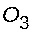
\includegraphics[width=\linewidth,height=.72\textheight,keepaspectratio]{images/image70.pdf}appartenant au solide 3, dans son
  mouvement par rapport à~\(R_{0}\). Cette accélération sera notée~:
  \(\overrightarrow{A_{O_{3} \in 3/0}}\).
\end{enumerate}

\[\overrightarrow{\mathbf{A}_{\mathbf{O}_{\mathbf{3}}\mathbf{\in}\mathbf{3/0}}}\mathbf{=}\left. \ \frac{\mathbf{d}\overrightarrow{\mathbf{V}_{\mathbf{O}_{\mathbf{3}}\mathbf{\in}\mathbf{3/0}}}}{\mathbf{dt}} \right|_{\mathbf{0}}\mathbf{=}\ddot{\mathbf{y}}\overrightarrow{\mathbf{y}_{\mathbf{0}}}\mathbf{- c}\ddot{\mathbf{\alpha}}\mathbf{\ }\overrightarrow{\mathbf{y}_{\mathbf{2}}}\mathbf{- c}\dot{\mathbf{\alpha}}\mathbf{\ }\left. \ \frac{\mathbf{d}\mathbf{\ }\overrightarrow{\mathbf{y}_{\mathbf{2}}}}{\mathbf{dt}} \right|_{\mathbf{0}}\mathbf{=}\ddot{\mathbf{y}}\overrightarrow{\mathbf{y}_{\mathbf{0}}}\mathbf{- c}\ddot{\mathbf{\alpha}}\mathbf{\ }\overrightarrow{\mathbf{y}_{\mathbf{2}}}\mathbf{- c}\dot{\mathbf{\alpha}^{\mathbf{2}}}\mathbf{\ }\overrightarrow{\mathbf{z}_{\mathbf{2}}}\]

\[\left. \ \frac{\mathbf{d}\mathbf{\ }\overrightarrow{\mathbf{y}}}{\mathbf{dt}} \right|_{\mathbf{0}}\mathbf{=}\mathbf{\ }\overrightarrow{\mathbf{\Omega}_{\mathbf{2/0}}}\mathbf{\land}\overrightarrow{\mathbf{y}_{\mathbf{2}}}\mathbf{=}\dot{\mathbf{\alpha}}\mathbf{\ }\overrightarrow{\mathbf{x}_{\mathbf{2}}}\mathbf{\land}\overrightarrow{\mathbf{y}_{\mathbf{2}}}\mathbf{=}\dot{\mathbf{\alpha}}\mathbf{\ }\overrightarrow{\mathbf{z}_{\mathbf{2}}}\]
\end{minipage} \\
\midrule\noalign{}
\endhead
\bottomrule\noalign{}
\endlastfoot
\end{longtable}

\subsection{Démarche de détermination des vecteurs vitesse et
accélération}\label{duxe9marche-de-duxe9termination-des-vecteurs-vitesse-et-accuxe9luxe9ration}

\subsubsection{Détermination du vecteur
vitesse}\label{duxe9termination-du-vecteur-vitesse}

Il existe \emph{\textbf{deux méthodes}} permettant de déterminer le
vecteur vitesse d'un point \emph{P} appartenant à un solide 2 (auquel
est associé un repère 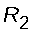
\includegraphics[width=\linewidth,height=.72\textheight,keepaspectratio]{images/image71.pdf}) en
mouvement par rapport à un solide 1 (auquel est associé un repère
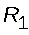
\includegraphics[width=\linewidth,height=.72\textheight,keepaspectratio]{images/image72.pdf}), lui-même en mouvement par
rapport à un solide 0 (auquel est associé un repère
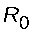
\includegraphics[width=\linewidth,height=.72\textheight,keepaspectratio]{images/image73.pdf}).


\includegraphics[width=\linewidth,height=.72\textheight,keepaspectratio]{images/image74.png}

\textbf{(1)} Avec l'habitude, on écrira directement le résultat~!

Dans tous les cas, on s'attachera à~:

\begin{itemize}
\item
  laisser le résultat dans des bases différentes;
\item
  vérifier que le résultat est bien homogène à une vitesse linéaire.
\end{itemize}

\subsubsection{Composition des vecteurs
vitesse}\label{composition-des-vecteurs-vitesse}

Soit un point \emph{P} appartenant à un solide 2 (auquel est associé un
repère
\(R_{2}(O_{2},\overrightarrow{x_{2}},\overrightarrow{y_{2}},\overrightarrow{z_{2}})\))
en mouvement par rapport à un solide 1 (auquel est associé un repère
\(R_{1}(O_{1},\overrightarrow{x_{1}},\overrightarrow{y_{1}},\overrightarrow{z_{1}})\)),
lui-même en mouvement par rapport à un solide 0 (auquel est associé un
repère \(R_{0}\)).


\includegraphics[width=\linewidth,height=.72\textheight,keepaspectratio]{images/image75.png}

On a~:
\(\overrightarrow{V_{P \in 2/0}} = \left\lbrack \frac{d\overrightarrow{O_{0}P_{\in 2}}}{dt} \right\rbrack_{0} = \left\lbrack \frac{d\overrightarrow{O_{0}O_{1}}}{dt} \right\rbrack_{0} + \left\lbrack \frac{d\overrightarrow{O_{1}P_{\in 2}}}{dt} \right\rbrack_{0}\)car
\(\overrightarrow{O_{0}P_{\in 2}} = \overrightarrow{O_{0}O_{1}} + \overrightarrow{O_{1}P_{\in 2}}\)

Donc~:
\(\overrightarrow{V_{P \in 2/0}} = \overrightarrow{V_{O_{1} \in 1/0}} + \left\lbrack \frac{d\overrightarrow{O_{1}P_{\in 2}}}{dt} \right\rbrack_{1} + \overrightarrow{\Omega_{1/0}} \land \overrightarrow{O_{1}P}\)
(formule de Boor)

\[\overrightarrow{V_{P \in 2/0}} = \overrightarrow{V_{O_{1} \in 1/0}} + \overrightarrow{V_{P \in 2/1}} + \overrightarrow{\Omega_{1/0}} \land \overrightarrow{O_{1}P}\]

\[\overrightarrow{V_{P \in 2/0}} = \overrightarrow{V_{P \in 2/1}} + \underset{\overrightarrow{V_{P \in 1/0}}}{\overset{\overrightarrow{V_{O_{1} \in 1/0}} + \overrightarrow{PO_{1}} \land \overrightarrow{\Omega_{1/0}}}{}}\]

Ce qui nous donne, grâce à la relation du champ des vecteurs vitesse~:

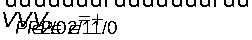
\includegraphics[width=\linewidth,height=.72\textheight,keepaspectratio]{images/image76.pdf}


\includegraphics[width=\linewidth,height=.72\textheight,keepaspectratio]{images/image77.png}\(\overrightarrow{V_{P \in 2/1}}\)est
la vitesse du point \emph{P} appartenant au solide 2 dans son mouvement
par rapport au solide 1~: \emph{\textbf{c'est la vitesse relative}}.

\(\overrightarrow{V_{P \in 1/0}}\)est la vitesse du point \emph{P,}
comme si il était fixe dans le repère
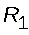
\includegraphics[width=\linewidth,height=.72\textheight,keepaspectratio]{images/image78.pdf}, dans son mouvement par rapport au
solide 0~: \emph{\textbf{c'est la vitesse d'entrainement.}}

\emph{Cela revient à imaginer que le solide 1 et le solide 2 ne forment
qu'un seul solide et qu'il n'y a plus de mouvement relatif possible de
l'un par rapport à l'autre.}

On peut généraliser cette relation de composition des vecteurs vitesse~à
\emph{\textbf{n}} solides (auxquels sont associés \textbf{\emph{n}}
repères successifs) en mouvement les uns par rapport aux autres :

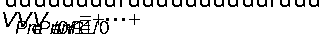
\includegraphics[width=\linewidth,height=.72\textheight,keepaspectratio]{images/image79.pdf}

Cette relation permet de déterminer simplement la vitesse d'un point
appartenant à un solide dont le mouvement est complexe. Le
\emph{\textbf{mouvement est décomposé en une somme de mouvements
simples}}~: rotation autour d'un axe, translation rectiligne\ldots{}

\subsubsection{Composition des vecteurs
rotation}\label{composition-des-vecteurs-rotation}

La relation de composition des vecteurs rotation, généralisée à
\emph{\textbf{n}} solides (auxquels sont associés \emph{\textbf{n}}
repères successifs) en mouvement les uns par rapport aux autres est :

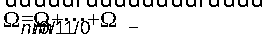
\includegraphics[width=\linewidth,height=.72\textheight,keepaspectratio]{images/image80.pdf}

\subsubsection{Composition des torseurs
cinématiques}\label{composition-des-torseurs-cinuxe9matiques}

Les deux relations établies précédemment nous permettent d'écrire dans
le cas de \emph{\textbf{n}} solides (auxquels sont associés
\emph{\textbf{n}} repères successifs) en mouvement les uns par rapport
aux autres :

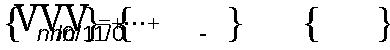
\includegraphics[width=\linewidth,height=.72\textheight,keepaspectratio]{images/image81.pdf}

\emph{\textbf{Les torseurs doivent être impérativement exprimés au même
point pour pouvoir être additionnés~!}}

\subsubsection{Champ des vecteurs
vitesse}\label{champ-des-vecteurs-vitesse}

Soit un solide 1 (auquel est associé un repère \(R_{1}\)) en mouvement
par rapport à un solide 0 (auquel est associé un repère \(R_{0}\)).

On note \(\overrightarrow{V_{A \in 1/0}}\) (ou
\(\overrightarrow{V_{A \in 1/R_{0}}}\)) le vecteur vitesse du point
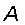
\includegraphics[width=\linewidth,height=.72\textheight,keepaspectratio]{images/image82.pdf}appartenant au solide
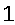
\includegraphics[width=\linewidth,height=.72\textheight,keepaspectratio]{images/image83.pdf} dans son mouvement par rapport au
repère \(R_{0}\).

\emph{\textbf{L'ensemble des vecteurs vitesse des points du solide 1 est
appelé champ des vecteurs vitesse du solide
1.}}
\includegraphics[width=\linewidth,height=.72\textheight,keepaspectratio]{images/image84.png}

Soit un solide 1 (auquel est associé un repère \(R_{1}\)) en mouvement
par rapport à un solide 0 (auquel est associé un repère \(R_{0}\)).

Soient A et B deux points du solide 1, on a~:
\(\left\lbrack \frac{d\overrightarrow{AB}}{dt} \right\rbrack_{0} = \left\lbrack \frac{d\overrightarrow{AB}}{dt} \right\rbrack_{1} + \overrightarrow{\Omega_{1/0}} \land \overrightarrow{AB}\)
(formule de Boor). Or \(\overrightarrow{AB}\) est fixe dans \(R_{1}\)
donc
\(\left\lbrack \frac{d\overrightarrow{AB}}{dt} \right\rbrack_{1} = \overrightarrow{0}\)

et
\(\overrightarrow{AB} = \overrightarrow{AO_{0}} + \overrightarrow{OB_{0}} = \overrightarrow{O_{0}B} - \overrightarrow{O_{0}A}\)

donc
\(\left\lbrack \frac{d\overrightarrow{AB}}{dt} \right\rbrack_{0} = \left\lbrack \frac{d\overrightarrow{O_{0}B_{\in 1}}}{dt} \right\rbrack_{0} - \left\lbrack \frac{d\overrightarrow{O_{0}A_{\in 1}}}{dt} \right\rbrack_{0} = \overrightarrow{V_{B \in 1/0}} - \overrightarrow{V_{A \in 1/0}}\)

On obtient~:
\(\overrightarrow{V_{B \in 1/0}} = \overrightarrow{V_{A \in 1/0}} + \overrightarrow{\Omega_{1/0}} \land \overrightarrow{AB}\)

On retiendra cette relation, qui n'est valable que pour des points
\ul{\emph{\textbf{appartenant au}} \emph{\textbf{même solide}}}, sous la
forme~: 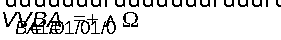
\includegraphics[width=\linewidth,height=.72\textheight,keepaspectratio]{images/image85.pdf}

\subsubsection{Détermination du vecteur
accélération}\label{duxe9termination-du-vecteur-accuxe9luxe9ration}

La relation du champ des vecteurs vitesse et la relation des
compositions des accélérations ne sont pas simples à retenir et à
utiliser.

Pour le calcul des vecteurs accélération, on privilégiera la méthode qui
consiste à calculer la \emph{\textbf{dérivée du vecteur vitesse}}, par
rapport au temps et dans le repère de référence.

Dans tous les cas, on s'attachera à~:

\begin{itemize}
\item
  laisser le résultat dans des bases différentes;
\item
  vérifier que le résultat est bien homogène à une accélération
  linéaire.
\end{itemize}

\begin{longtable}{@{}
  >{\raggedright\arraybackslash}p{(\columnwidth - 2\tabcolsep) * \real{0.1227}}
  >{\raggedright\arraybackslash}p{(\columnwidth - 2\tabcolsep) * \real{0.8773}}@{}}
\toprule\noalign{}
\begin{minipage}[b]{\linewidth}\raggedright
\begin{quote}

\includegraphics[width=\linewidth,height=.72\textheight,keepaspectratio]{images/image18.png}
\end{quote}
\end{minipage} & \begin{minipage}[b]{\linewidth}\raggedright
\textbf{Machine 5 axes}

\(\overrightarrow{O_{0}O_{4}} = x(t) \cdot \overrightarrow{x_{0}} + d \cdot \overrightarrow{z_{0}}\)

\[\overrightarrow{AO_{1}} = a \cdot \overrightarrow{z_{1}}\]

\[\overrightarrow{O_{4}D} = e \cdot \overrightarrow{y_{4}}\ \ \ \ \ \ \ \ \ \ \ \ \ \ \ \ \ \ \ \ \ \ \ \ \ \ \ \ \]

\(\mathbf{\ }\overrightarrow{O_{0}A} = y(t) \cdot \overrightarrow{y_{0}}\)
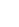
\includegraphics[width=\linewidth,height=.72\textheight,keepaspectratio]{images/image27.pdf}

\(\overrightarrow{O_{1}O_{2}} = b \cdot \overrightarrow{x_{2}}\)

\[\overrightarrow{O_{5}P} = - f \cdot \overrightarrow{z_{5}}\]

\(\overrightarrow{DO_{5}} = - z(t) \cdot \overrightarrow{z_{4}}\)

\(\overrightarrow{O_{2}O_{3}} = c \cdot \overrightarrow{z_{3}}\)

\(\alpha = \left( \overrightarrow{y_{1}},\overrightarrow{y_{2}} \right)\)
et
\(\beta = \left( \overrightarrow{x_{2}},\overrightarrow{x_{3}} \right)\)


\includegraphics[width=\linewidth,height=.72\textheight,keepaspectratio]{images/image49.png}

\begin{enumerate}
\def\labelenumi{\arabic{enumi}.}
\item
  Déterminer le vecteur vitesse \(\overrightarrow{V_{P \in 5/0}}\ \)du
  point \(P\) appartenant à l'outil, dans son mouvement par rapport
  à~\(R_{0}\).
\end{enumerate}

\(\overrightarrow{\mathbf{V}_{\mathbf{P}\mathbf{\in}\mathbf{5/0}}}\mathbf{=}\overrightarrow{\mathbf{V}_{\mathbf{P}\mathbf{\in}\underset{\mathbf{T}}{\overset{\mathbf{5/4}}{}}}} + \overrightarrow{V_{P \in \underset{\mathbf{T}}{\overset{\mathbf{4}\mathbf{/}\mathbf{0}}{}}}} = \dot{\mathbf{x}}\overrightarrow{\mathbf{x}_{\mathbf{0}}}\mathbf{-}\dot{\mathbf{z}}\overrightarrow{\mathbf{z}_{\mathbf{0}}}\)

\begin{enumerate}
\def\labelenumi{\arabic{enumi}.}
\setcounter{enumi}{1}
\item
  Déterminer le vecteur vitesse \(\overrightarrow{V_{O_{3} \in 3/0}}\)
  du point \(O_{3}\) appartenant au solide 3 (pièce usinée + support),
  dans son mouvement par rapport à~\(R_{0}\).
\end{enumerate}

\[\overrightarrow{\mathbf{V}_{\mathbf{O}_{\mathbf{3}}\mathbf{\in}\mathbf{3}\mathbf{/0}}}\mathbf{=}\overrightarrow{\mathbf{V}_{\mathbf{O}_{\mathbf{3}}\mathbf{\in}\underset{\mathbf{T}}{\overset{\mathbf{3}\mathbf{/}\mathbf{2}}{}}}} + \overrightarrow{V_{\mathbf{O}_{\mathbf{3}}\mathbf{\in}\underset{\mathbf{T}}{\overset{\mathbf{2}\mathbf{/}\mathbf{1}}{}}}} + \overrightarrow{V_{\mathbf{O}_{\mathbf{3}}\mathbf{\in}\underset{\mathbf{T}}{\overset{\mathbf{1}\mathbf{/}\mathbf{0}}{}}}}\]

\textbf{1}
\(\overrightarrow{\mathbf{V}_{\mathbf{O}_{\mathbf{3}}\mathbf{\in}\mathbf{3/2}}}\mathbf{=}\overrightarrow{\underset{\overrightarrow{\mathbf{0}}\mathbf{\ }}{\overset{\mathbf{V}_{\mathbf{O}_{\mathbf{2}}\mathbf{\in}\mathbf{3/2}}}{}}}\mathbf{+}\overrightarrow{\mathbf{O}_{\mathbf{3}}\mathbf{O}_{\mathbf{2}}}\mathbf{\land}\overrightarrow{\mathbf{\Omega}_{\mathbf{3/2}}}\mathbf{= - e}\overrightarrow{\mathbf{z}_{\mathbf{3}}}\mathbf{\land}\dot{\mathbf{\beta}}\mathbf{\ }\overrightarrow{\mathbf{z}_{\mathbf{2}}}\mathbf{=}\overrightarrow{\mathbf{0}}\mathbf{\ }\)\textbf{logique
puisque} \(\mathbf{O}_{\mathbf{3}}\) \textbf{est sur l'axe de rotation
3/2}

\textbf{2-}
\(\overrightarrow{\mathbf{V}_{\mathbf{O}_{\mathbf{3}}\mathbf{\in}\mathbf{2/1}}}\mathbf{=}\overrightarrow{\underset{\overrightarrow{\mathbf{0}}\mathbf{\ }}{\overset{\mathbf{V}_{\mathbf{O}_{\mathbf{1}}\mathbf{\in}\mathbf{2/1}}}{}}}\mathbf{+}\overrightarrow{\mathbf{O}_{\mathbf{3}}\mathbf{O}_{\mathbf{1}}}\mathbf{\land}\overrightarrow{\mathbf{\Omega}_{\frac{\mathbf{2}}{\mathbf{1}}}}\mathbf{= -}\left( \mathbf{c}\overrightarrow{\mathbf{z}_{\mathbf{3}}}\mathbf{+}\mathbf{b}\overrightarrow{\mathbf{x}_{\mathbf{2}}} \right)\mathbf{\land}\dot{\mathbf{\alpha}}\mathbf{\ }\overrightarrow{\mathbf{x}_{\mathbf{2}}}\mathbf{= - c}\dot{\mathbf{\alpha}}\mathbf{\ }\overrightarrow{\mathbf{y}_{\mathbf{2}}}\)

\textbf{3-}
\(\overrightarrow{\mathbf{V}_{\mathbf{O}_{\mathbf{3}}\mathbf{\in}\mathbf{1/0}}}\mathbf{=}\dot{\mathbf{y}}\overrightarrow{\mathbf{y}_{\mathbf{0}}}\)

\[\overrightarrow{\mathbf{V}_{\mathbf{O}_{\mathbf{3}}\mathbf{\in}\mathbf{3}\mathbf{/0}}}\mathbf{=}\dot{\mathbf{y}}\overrightarrow{\mathbf{y}_{\mathbf{0}}}\mathbf{- c}\dot{\mathbf{\alpha}}\mathbf{\ }\overrightarrow{\mathbf{y}_{\mathbf{2}}}\]
\end{minipage} \\
\midrule\noalign{}
\endhead
\bottomrule\noalign{}
\endlastfoot
\end{longtable}

\subsubsection{Champ des vecteurs
accélération}\label{champ-des-vecteurs-accuxe9luxe9ration}

Soit un solide 1 (auquel est associé un repère \(R_{1}\)) en mouvement
par rapport à un solide 0 (auquel est associé un repère \(R_{0}\)).

Soient A et B deux points du solide 1, on a~:
\(\overrightarrow{V_{B \in 1/0}} = \overrightarrow{V_{A \in 1/0}} + \overrightarrow{BA} \land \overrightarrow{\Omega_{1/0}}\)

Si on dérive, par rapport au temps, et dans le repère \(R_{0}\), les
deux membres de cette égalité~:

\[\left\lbrack \frac{d\overrightarrow{V_{B \in 1/0}}}{dt} \right\rbrack_{0} = \left\lbrack \frac{d\overrightarrow{V_{A \in 1/0}}}{dt} \right\rbrack_{0} + \left\lbrack \frac{d\overrightarrow{BA}}{dt} \right\rbrack_{0} \land \overrightarrow{\Omega_{1/0}} + \overrightarrow{BA} \land \left\lbrack \frac{d\overrightarrow{\Omega_{1/0}}}{dt} \right\rbrack_{0}\]

\textbf{Rappel~:} \emph{Dérivée d'un produit vectoriel~}
\(\frac{d(\overrightarrow{u} \land \overrightarrow{v})}{dt} = \frac{d\overrightarrow{u}}{dt} \land \overrightarrow{v} + \overrightarrow{u} \land \frac{d\overrightarrow{v}}{dt}\)

Soit~:
\(\overrightarrow{A_{B \in 1/0}} = \overrightarrow{A_{A \in 1/0}} + \left( \left\lbrack \frac{d\overrightarrow{BA}}{dt} \right\rbrack_{1} + \overrightarrow{\Omega_{1/0}} \land \overrightarrow{BA} \right) \land \overrightarrow{\Omega_{1/0}} + \overrightarrow{BA} \land \left\lbrack \frac{d\overrightarrow{\Omega_{1/0}}}{dt} \right\rbrack_{0}\)

Or \(\overrightarrow{AB}\) est fixe dans \(R_{1}\), donc~:
\(\overrightarrow{A_{B \in 1/0}} = \overrightarrow{A_{A \in 1/0}} + \left( \overrightarrow{\Omega_{1/0}} \land \overrightarrow{BA} \right) \land \overrightarrow{\Omega_{1/0}} + \overrightarrow{BA} \land \left\lbrack \frac{d\overrightarrow{\Omega_{1/0}}}{dt} \right\rbrack_{0}\)

\subsubsection{Composition des vecteurs
accélérations}\label{composition-des-vecteurs-accuxe9luxe9rations}

Soit un point \emph{P} appartenant à un solide 2 (auquel est associé un
repère \(R_{2}\)) en mouvement par rapport à un solide 1 (auquel est
associé un repère \(R_{1}\)), lui-même en mouvement par rapport à un
solide 0 (auquel est associé un repère \(R_{0}\)).

On montre que~:
\(\overrightarrow{A_{P \in 2/0}} = \overrightarrow{A_{P \in 2/1}} + \overrightarrow{A_{P \in 1/0}} + 2 \cdot \overrightarrow{\Omega_{1/0}} \land \overrightarrow{V_{P \in 2/1}}\)

\subsubsection{Fermeture cinématique}\label{fermeture-cinuxe9matique}

Pour déterminer une loi entrée sortie en vitesse ou par exemple un degré
d'hyperstaticité, une fermeture cinématique est utilisée. Il suffit
d'écrire une composition des torseurs cinématiques sur la boucle
considérée en écrivant que la somme est égale au torseur nul.

\begin{longtable}{@{}
  >{\raggedright\arraybackslash}p{(\columnwidth - 2\tabcolsep) * \real{0.1227}}
  >{\raggedright\arraybackslash}p{(\columnwidth - 2\tabcolsep) * \real{0.8773}}@{}}
\toprule\noalign{}
\begin{minipage}[b]{\linewidth}\raggedright
\begin{quote}

\includegraphics[width=\linewidth,height=.72\textheight,keepaspectratio]{images/image18.png}
\end{quote}
\end{minipage} & \begin{minipage}[b]{\linewidth}\raggedright
\textbf{Vérin électrique}


\includegraphics[width=\linewidth,height=.72\textheight,keepaspectratio]{images/image86.png}

\begin{enumerate}
\def\labelenumi{\arabic{enumi}.}
\item
  Ecrire la fermeture cinématique de chaîne relative à ce mécanisme.
\end{enumerate}

\(\left\{ \mathbf{V}_{\mathbf{2/0}} \right\}_{\mathbf{0}}\mathbf{+}\left\{ \mathbf{V}_{\mathbf{0/1}} \right\}_{\mathbf{0}}{\mathbf{+}\left\{ \mathbf{V}_{\mathbf{1/2}} \right\}}_{\mathbf{0}}\mathbf{= \{ 0\}}\)

\[\left\{ \mathbf{V}_{\mathbf{2/0}} \right\}_{\mathbf{0}}\mathbf{-}\left\{ \mathbf{V}_{\mathbf{1/0}} \right\}_{\mathbf{0}}{\mathbf{-}\left\{ \mathbf{V}_{\mathbf{2/1}} \right\}}_{\mathbf{0}}\mathbf{= \{ 0\}}\]

\begin{enumerate}
\def\labelenumi{\arabic{enumi}.}
\setcounter{enumi}{1}
\item
  En déduire le rang r\textsubscript{c} du système d'équations
  cinématique, le degré de mobilité cinématique m et le degré
  d'hyperstatisme h.
\end{enumerate}

\[\left\{ \begin{array}{r}
0 \\
0 \\
0
\end{array} \middle| \begin{array}{r}
V_{20} \\
0 \\
0
\end{array} \right\}_{0,R} - \left\{ \begin{array}{r}
\Omega_{10} \\
0 \\
0
\end{array} \middle| \begin{array}{r}
0 \\
0 \\
0
\end{array} \right\}_{0,R} - \left\{ \begin{array}{r}
\Omega_{21} \\
0 \\
0
\end{array} \middle| \begin{array}{r}
V_{21} \\
0 \\
0
\end{array} \right\}_{0,R} = \left\{ \begin{array}{r}
0 \\
0 \\
0
\end{array} \middle| \begin{array}{r}
0 \\
0 \\
0
\end{array} \right\}_{0,R}\]

Le système s'écrit~:

\[0 - \Omega_{10} - \Omega_{21} = 0\]

\[0 - 0 - 0 = 0\]

\[0 - 0 - 0 = 0\]

\[V_{20} - 0 - V_{21} = 0\]

\[0 - 0 - 0 = 0\]

\[0 - 0 - 0 = 0\]
\end{minipage} \\
\midrule\noalign{}
\endhead
\bottomrule\noalign{}
\endlastfoot
\end{longtable}

\subsection[Cinématique du contact
ponctuel]{\texorpdfstring{\protect
\includegraphics[width=\linewidth,height=.72\textheight,keepaspectratio]{images/image87.png}Cinématique
du contact
ponctuel}{Cinématique du contact ponctuel}}\label{cinuxe9matique-du-contact-ponctuel}

Lorsque deux solides 1 et 2, en mouvement par rapport à un repère de
référence \(R_{0}\), sont en contact ponctuel au point
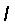
\includegraphics[width=\linewidth,height=.72\textheight,keepaspectratio]{images/image88.pdf}, il faut distinguer trois points.

\begin{itemize}
\item
  Un point \(I \in 1\) lié au solide 1
\item
  Un point \(I \in 2\) lié au solide 2
\item
  Un point géométrique de contact \(I\) qui n'appartient à aucun des
  solides
\end{itemize}

On défini la vitesse de glissement comme étant~:

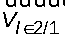
\includegraphics[width=\linewidth,height=.72\textheight,keepaspectratio]{images/image89.pdf} \emph{\textbf{\ul{porté par le
plan tangent commun aux deux solides au point de contact}}}

Pour calculer ce vecteur vitesse, on utilise en général, la composition
des vitesses~:

\(\overrightarrow{V_{I \in 2/1}} = \overrightarrow{V_{I \in 2/0}} + \overrightarrow{V_{I \in 0/1}} = \overrightarrow{V_{I \in 2/0}} - \overrightarrow{V_{I \in 1/0}}\)

\textbf{\ul{Roulement Sans Glissement (RSG)}}

On considère que le solide 2 roule sans glisser sur le solide 1 lorsque
la vitesse de glissement est nulle~:
\(\overrightarrow{V_{I \in 2/1}} = \overrightarrow{0}\)

\ul{Remarque~:} tout point où il y a RSG est un CIR (Centre Instantané
de Rotation).

La condition de RSG est souvent utilisée pour mettre en évidence les
relations qui lient les paramètres de mouvement des solides qui
constituent les trains d'engrenages (simples ou épicycloïdaux), les
roulements (à billes, à rouleaux\ldots), les dispositifs
poulie/courroie, pignon / chaine \ldots.

\begin{longtable}{@{}
  >{\raggedright\arraybackslash}p{(\columnwidth - 2\tabcolsep) * \real{0.1227}}
  >{\raggedright\arraybackslash}p{(\columnwidth - 2\tabcolsep) * \real{0.8773}}@{}}
\toprule\noalign{}
\begin{minipage}[b]{\linewidth}\raggedright
\begin{quote}

\includegraphics[width=\linewidth,height=.72\textheight,keepaspectratio]{images/image18.png}
\end{quote}
\end{minipage} & \begin{minipage}[b]{\linewidth}\raggedright
\textbf{Capsuleuse -- Croix de Malte}

Ci-dessous la modélisation du mécanisme à Croix de Malte d'une
capsuleuse.


\includegraphics[width=\linewidth,height=.72\textheight,keepaspectratio]{images/image90.png}
\includegraphics[width=\linewidth,height=.72\textheight,keepaspectratio]{images/image91.png}

\begin{enumerate}
\def\labelenumi{\arabic{enumi}.}
\item
  Ecrire la condition de RSG en I.
\end{enumerate}

\textbf{Banc de test pneumatique}

On s'intéresse à un banc de tests d'usure de pneumatiques. Un ensemble
pneumatique + jante 2, entrainé en rotation par rapport au bras 3 à
l'aide d'un moto-réducteur, roule sur un plateau tournant 1. Le bras 3
et le plateau tournant

1 sont entrainés en rotation par rapport aux bâti 0 à l'aide de deux
autres moto- réducteurs. En assimilant la roue 2 à un disque on obtient
le schéma cinématique suivant du système


\includegraphics[width=\linewidth,height=.72\textheight,keepaspectratio]{images/image92.png}

\includegraphics[width=\linewidth,height=.72\textheight,keepaspectratio]{images/image93.png}

\begin{enumerate}
\def\labelenumi{\arabic{enumi}.}
\item
  Ecrire la condition de RSG en I.
\end{enumerate}
\end{minipage} \\
\midrule\noalign{}
\endhead
\bottomrule\noalign{}
\endlastfoot
\end{longtable}

\subsection{LA LOI TRAPEZE}\label{la-loi-trapeze}

En cinématique, les vitesses dépendront des dérivées des paramètres
variables angulaires et linéaires. Pour les chaînes ouvertes, il sera
nécessaire de disposer d'un actionneur par paramètre variable pour
animer un système. Pour les chaînes fermées à une seule boucle, il
suffira d'un actionneur en entrée du système pour l'animer. Les lois
d'évolution des actionneurs sont au choix du concepteur du système.

Physiquement il est impossible de passer d'une vitesse nulle à une
vitesse non nulle. Par une première approche, il est possible qu'un
actionneur soit piloté par une loi de vitesse en trapèze :


\includegraphics[width=\linewidth,height=.72\textheight,keepaspectratio]{images/image94.png}

Le mouvement d'un solide est paramétré par~:

\begin{itemize}
\item
  sa position : \(\text{$\lambda$}_{\left( \text{t} \right)}\),
  ou\(\ \text{$\alpha$}_{\left( \text{t} \right)}\)
\item
  sa vitesse instantanée :
  \(v_{\left( \text{t} \right)} = {\dot{\text{$\lambda$}}}_{\left( \text{t} \right)}\)
\item
  son accélération :
  \(\text{a}_{\left( \text{t} \right)} = {\dot{v}}_{\left( \text{t} \right)} = {\ddot{\lambda}}_{\left( \text{t} \right)}\)
\end{itemize}

La méthode «~classique~» est de faire les équations horaires, mais elle
s'avère peu efficace pour des lois de commande plus complexe qu'un
simple trapèze. Les équations horaires du mouvement sont les équations
analytiques donnant l'évolution de x (position), \(v\) (vitesse) et a
(accélération) en fonction de t (temps).

Le plus simple est de faire un raisonnement «~graphique~» utilisant les
aires et relations entre les différentes grandeurs position, vitesse,
accélération.

Un peu de vocabulaire quand même~:

\begin{itemize}
\item
  on parle de \textbf{mouvement uniforme} lorsque la \textbf{vitesse est
  constante (accélération nulle)}.... Vous verrez que cela
  s\textquotesingle appelle \textbf{aussi régime établi ou régime
  permanent}\ldots{}
\item
  on parle de mouvement \textbf{uniformément varié} lorsque la
  \textbf{vitesse varie linéairement (accélération constante)}
\end{itemize}

Connaissant l'évolution de la vitesse au cours du temps, comment
connaître la position du solide étudié~?

t

t\textsubscript{1}

t\textsubscript{2}

\[\text{x}\]

\[\text{x}_{\left( \text{t}_{\text{1}} \right)}\]

0

t\textsubscript{3}

\[\text{x}_{\left( \text{t}_{\text{2}} \right)}\]

\[\text{x}_{\left( \text{t}_{\text{3}} \right)}\]

t

t\textsubscript{1}

t\textsubscript{2}

\[v\]

V\textsubscript{1}

0

t\textsubscript{3}

t

t\textsubscript{1}

t\textsubscript{2}

\[a\]

a\textsubscript{1}

0

t\textsubscript{3}

t

t\textsubscript{1}

t\textsubscript{2}

\[v\]

V\textsubscript{1}

0

t\textsubscript{3}

V\textsubscript{f}

t

t\textsubscript{1}

t\textsubscript{2}

\[\text{x}\]

\[\text{x}_{\left( \text{t}_{\text{1}} \right)}\]

0

t\textsubscript{3}

\[\text{x}_{\left( \text{t}_{\text{2}} \right)}\]

\[\text{x}_{\left( \text{t}_{\text{3}} \right)}\]

Par définition
\(v_{\left( \text{t} \right)} = \frac{d\text{x}_{\left( \text{t} \right)}}{d\text{t}}\)
soit
\(\text{x}_{\left( \text{t} \right)} - \text{x}_{\left( \text{0} \right)} = \int_{T = 0}^{t}v_{\left( \text{T} \right)}d\text{T}\)
donc
\(\text{x}_{\left( \text{t} \right)} - \text{x}_{\left( \text{0} \right)}\)
est l'aire de la courbe \(v_{\left( \text{T} \right)}\) entre 0 et t.

\emph{\ul{Entre 0 et t\textsubscript{1}~:}}

t

t\textsubscript{1}

t\textsubscript{2}

\[\text{x}\]

\[\text{x}_{\left( \text{t}_{\text{1}} \right)}\]

t\textsubscript{0}

t\textsubscript{3}

\[\text{x}_{\left( \text{t}_{\text{2}} \right)}\]

\[\text{x}_{\left( \text{t}_{\text{3}} \right)}\]

t

t\textsubscript{1}

\[v\]

V\textsubscript{1}

t\textsubscript{0}

\[\text{x}_{\left( \text{t}_{\text{0}} \right)}\]

Le coefficient directeur de la droite est
\(\frac{\text{V}_{\text{1}}}{\text{t}_{\text{1}}}\) (c'est
l'accélération) donc
\(v_{\left( \text{t} \right)} = \frac{\text{V}_{\text{1}}}{\text{t}_{\text{1}}}\).t

\[\Delta x = \text{x}_{\left( t_{1} \right)} - \text{x}_{\left( t_{0} \right)} = \text{Aire}\text{ (triangle)}\]

\emph{\ul{Entre t\textsubscript{1} et t\textsubscript{2}~:}}

On a
\(v_{\left( \text{t} \right)}\text{=}\text{cte}\text{=}\text{V}_{\text{1}}\)

\begin{longtable}{@{}
  >{\raggedright\arraybackslash}p{(\columnwidth - 2\tabcolsep) * \real{0.5195}}
  >{\raggedright\arraybackslash}p{(\columnwidth - 2\tabcolsep) * \real{0.4805}}@{}}
\toprule\noalign{}
\begin{minipage}[b]{\linewidth}\raggedright
t

t\textsubscript{1}

t\textsubscript{2}

\[v\]

V\textsubscript{1}

0

\textbf{t}

\[\text{x}_{\left( \text{t} \right)} - \text{x}_{\left( t_{1} \right)} = \text{Aire}\text{ (rectangle)} = \text{V}_{\text{1}}.\left( \text{t-}\text{t}_{\text{1}} \right)\]
\end{minipage} & \begin{minipage}[b]{\linewidth}\raggedright
\[v\]

V\textsubscript{1}

\textbf{t}

0

t\textsubscript{2}

t\textsubscript{1}

t

\[\text{x}_{\left( \text{t} \right)} - \text{x}_{(0)} = \text{ Aire}\text{ (rectangle)+}\text{Aire}\text{ (triangle)}\]

t

t\textsubscript{1}

t\textsubscript{2}

\[\text{x}\]

\[\text{x}_{\left( \text{t}_{\text{1}} \right)}\]

0

t\textsubscript{3}

\[\text{x}_{\left( \text{t}_{\text{2}} \right)}\]

\[\text{x}_{\left( \text{t}_{\text{3}} \right)}\]
\end{minipage} \\
\midrule\noalign{}
\endhead
\bottomrule\noalign{}
\endlastfoot
\end{longtable}

\emph{\ul{Entre t\textsubscript{2} et t\textsubscript{3}~:}}

\[\text{Aire}\text{ (trapèze)} = \frac{\left( \text{B+b} \right)\text{.h}}{\text{2}} = \frac{\left( \text{V}_{\text{1}}\text{+}v_{\left( \text{t} \right)} \right)\text{.}\left( \text{t-}\text{t}_{\text{2}} \right)}{\text{2}}\]

\[\text{Aire}\text{ (trapèze)} = \frac{\left( \text{V}_{\text{1}}\text{+}v_{\left( \text{t} \right)} \right)\text{.}\left( \text{t-}\text{t}_{\text{2}} \right)}{\text{2}} = \frac{\left( \text{V}_{\text{1}}\text{-}\frac{\text{V}_{\text{1}}}{\text{t}_{\text{3}}\text{-}\text{t}_{\text{2}}}\text{.}\left( \text{t-}\text{t}_{\text{2}} \right) + \text{V}_{\text{1}} \right)\text{.}\left( \text{t-}\text{t}_{\text{2}} \right)}{\text{2}}\]

t

t\textsubscript{1}

t\textsubscript{2}

\[v\]

V\textsubscript{1}

0

t\textsubscript{3}

\textbf{t}

\[\text{x}_{\left( \text{t} \right)} - \text{x}_{(0)} = \text{ Aire}\text{ (rectangle)+}\text{Aire}\text{ (triangle)+}\text{Aire}\text{ (trapèze)}\]

Pour l'accélération, il suffit de mettre le coefficient directeur de la
vitesse~: \(a = \frac{\mathrm{\Delta}v}{\mathrm{\Delta}t}\).

L'accélération est positive lorsque la vitesse est croissante, négative
lorsqu'elle est décroissante et nulle lorsqu'elle est constante.

\begin{longtable}{@{}
  >{\raggedright\arraybackslash}p{(\columnwidth - 2\tabcolsep) * \real{0.1227}}
  >{\raggedright\arraybackslash}p{(\columnwidth - 2\tabcolsep) * \real{0.8773}}@{}}
\toprule\noalign{}
\begin{minipage}[b]{\linewidth}\raggedright
\begin{quote}

\includegraphics[width=\linewidth,height=.72\textheight,keepaspectratio]{images/image18.png}
\end{quote}
\end{minipage} & \begin{minipage}[b]{\linewidth}\raggedright
\textbf{Hayon de coffre électrique}


\includegraphics[width=\linewidth,height=.72\textheight,keepaspectratio]{images/image97.jpeg}Objectif
~: Déterminer le temps total d'ouverture du hayon.

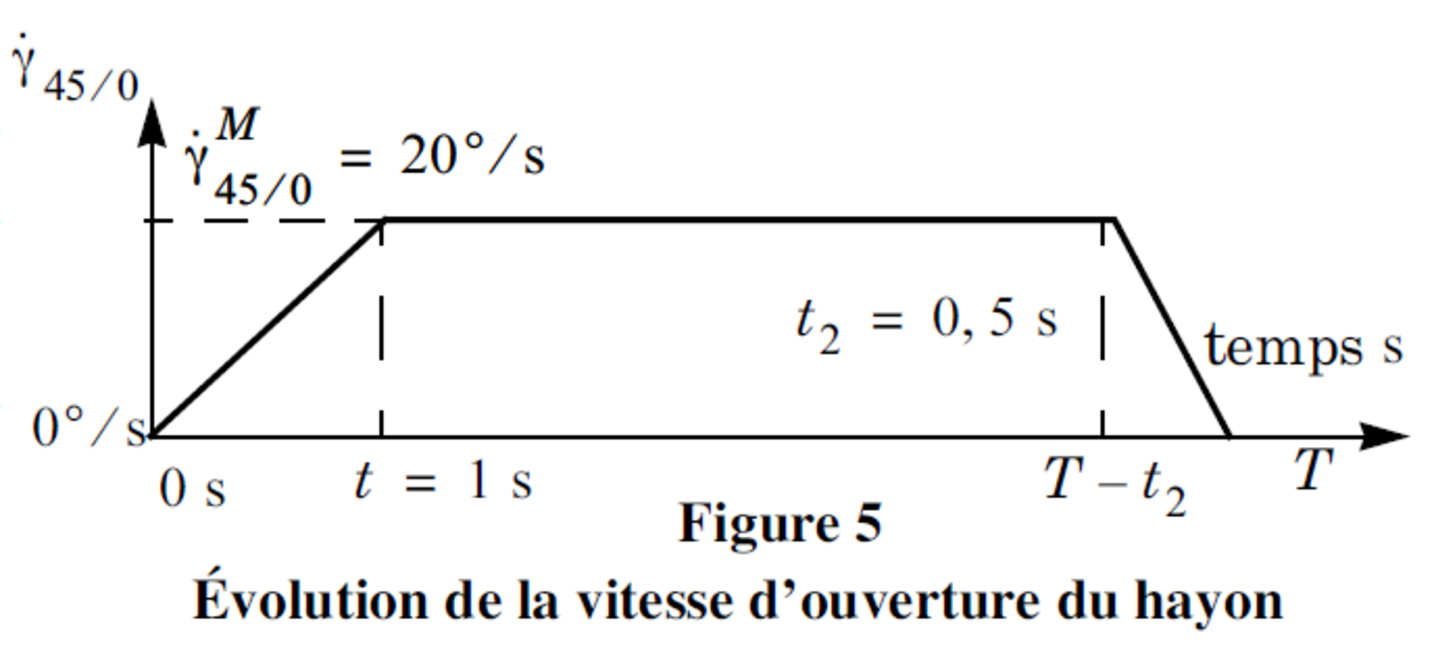
\includegraphics[width=\linewidth,height=.72\textheight,keepaspectratio]{images/image98.pdf}La
figure 5 présente la loi d'évolution en trapèze de la vitesse
d'ouverture du hayon imposée par le cahier des charges.

\begin{enumerate}
\def\labelenumi{\arabic{enumi}.}
\item
  Tracer, l'allure temporelle de la courbe représentative de
  \(\gamma_{45/0}(t)\) sachant que \(\gamma_{45/0}(0) = 0\).
\end{enumerate}


\includegraphics[width=\linewidth,height=.72\textheight,keepaspectratio]{images/image99.png}

20 °/s

t\textsubscript{2}=0,5 s

\begin{enumerate}
\def\labelenumi{\arabic{enumi}.}
\setcounter{enumi}{1}
\item
  Calculer le temps d'ouverture \(T\) du hayon pour une ouverture
  \(\gamma_{45/0}(T) = 90{^\circ}\)
\end{enumerate}
\end{minipage} \\
\midrule\noalign{}
\endhead
\bottomrule\noalign{}
\endlastfoot
\end{longtable}

\subsection{Sources}\label{sources}

Ce cours a été élaboré à l'aide de nombreuses ressources~provenant de
différents collègues~de l'UPSTI.

\subsection{Exercices du chapitre}\label{exercices-du-chapitre}


\includegraphics[width=\linewidth,height=.72\textheight,keepaspectratio]{images/image100.png}

\textbf{LOI TRAPEZE}


\includegraphics[width=\linewidth,height=.72\textheight,keepaspectratio]{images/image101.png}
Niveau 1


\includegraphics[width=\linewidth,height=.72\textheight,keepaspectratio]{images/image102.png}

a (m.s\textsuperscript{-2})

t(s)

0,2

0,7

0,8

1,3

1,5

1,7

1,9

2,4

2,5

3

3,2

0

-0,5

-0,9

0,8

1,2

0

3,2

3

2,5

2,4

1,9

1,7

1,5

1,3

0,8

0,7

0,2

t(s)

0

3,2

3

2,5

2,4

1,9

1,7

1,5

1,3

0,8

0,7

0,2

t(s)

v (m.s\textsuperscript{-1})

x (m)

\begin{enumerate}
\item
  Maison DOME
\end{enumerate}


\includegraphics[width=\linewidth,height=.72\textheight,keepaspectratio]{images/image101.png}
Niveau 1

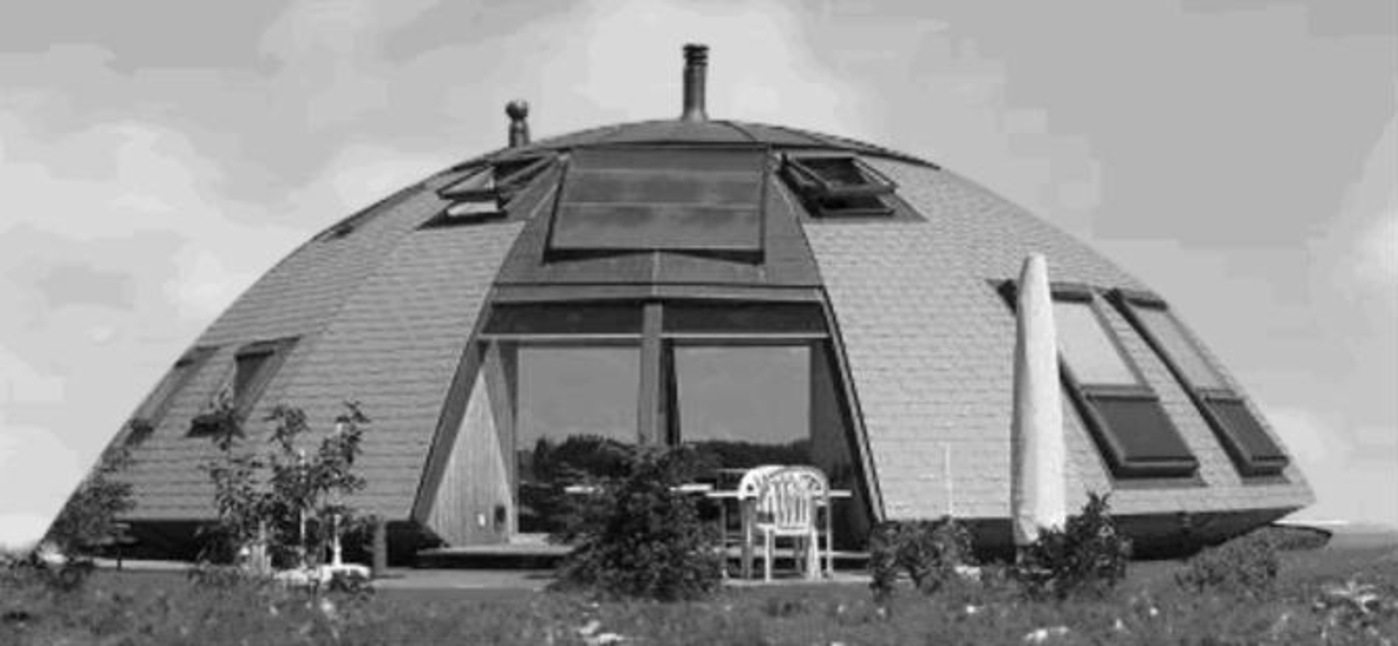
\includegraphics[width=\linewidth,height=.72\textheight,keepaspectratio]{images/image103.pdf}A
toutes les époques et sous toutes les latitudes, les hommes ont utilisé
la forme circulaire dans leurs constructions (case, igloo,
yourte\ldots). Le concept de l'habitat circulaire tournant s'adapte aux
nouvelles contraintes énergétiques de notre époque. La maison DÔME,
intégrant la domotique, utilise judicieusement l'énergie solaire et est
réalisée en bois, un matériau naturel et recyclable. La maison DÔME est
un habitat rotatif qui suit le soleil et la source de chaleur en hiver
ou, au contraire, mettre à l\textquotesingle ombre
l\textquotesingle été, change d\textquotesingle orientation visuelle et
positionne les chambres à l\textquotesingle abri du vent, en cas de
tempête\ldots{} Cette maison est livrée avec un dispositif de rotation
automatique réalisé par un ensemble motorisé.

\textbf{Maîtrise de la position d'arrêt de la maison.}

\ul{Objectif} : déterminer le comportement de la maison alors qu'elle
est en mouvement et qu'on souhaite l'immobiliser. Lors de la mise hors
tension du moteur, alors qu'elle était en mouvement, la maison continue
de tourner pendant une durée de 8 secondes.

30×10\textsuperscript{-3}

t(s)

T\textsubscript{a} = 8s

Coupure du moteur

Fréquence de rotation de la maison \(N_{m}\)
(tr.min\textsuperscript{-1})

Le graphe ci-contre indique l'évolution de la vitesse de rotation
N\textsubscript{m} de la maison lors d'une phase d'arrêt.

\textbf{1.} Pourquoi la maison continue-t-elle de tourner si longtemps
après que le moteur soit mis hors tension ?

\textbf{2.} Calculer l'accélération angulaire\(\ {\ddot{\theta}}_{a}\)
de la maison en rad.s\textsuperscript{-2}.

Résultat~: Quelle que soit la valeur trouvée prendre
\({\ddot{\theta}}_{a} = - 0,4 \times 10^{- 3}\ rad.s^{- 2}\) .

\textbf{3.} En déduire l'angle \(\theta_{a}\)parcouru par la maison
pendant la phase d'arrêt. Exprimer le résultat en radians puis degrés.

Le cahier des charges indique que la distance parcoure pendant l'arrêt
de la maison doit être inférieure à 15cm.

\textbf{4.} Déterminer la distance L correspondante, parcourue en
périphérie de la maison c'est à dire au niveau de la porte d'entrée,
pour un dôme de diamètre OP = d =16 m.

\textbf{5.} Conclure quant au respect du cahier des charges.

Résultat~: L=10,05 cm

\begin{enumerate}
\setcounter{enumi}{1}
\item
  Véhicule électrique F-city
\end{enumerate}


\includegraphics[width=\linewidth,height=.72\textheight,keepaspectratio]{images/image101.png}
Niveau 1

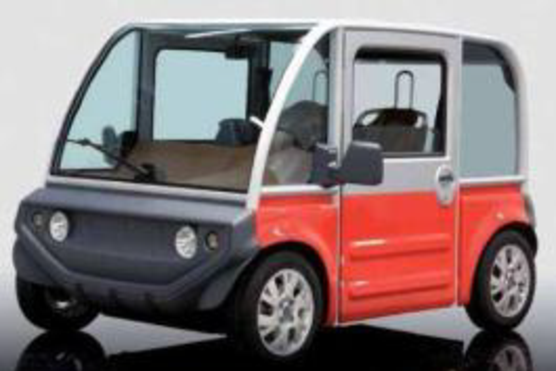
\includegraphics[width=\linewidth,height=.72\textheight,keepaspectratio]{images/image104.pdf}Fabriquée
par la société FAM Automobiles, entreprise basée à Etupes dans le nord
Franche-Comté, la F-City est une petite voiture électrique qui peut être
utilisée en libre accès et réservée d'un simple appel téléphonique.

\textbf{Description générale.}

\begin{longtable}{@{}
  >{\raggedright\arraybackslash}p{(\columnwidth - 2\tabcolsep) * \real{0.3768}}
  >{\raggedright\arraybackslash}p{(\columnwidth - 2\tabcolsep) * \real{0.6232}}@{}}
\toprule\noalign{}
\endhead
\bottomrule\noalign{}
\endlastfoot
Nombre de places : & 2 \\
Motorisation : & moteur asynchrone électrique triphasé groupe
motopropulseur en position arrière. \\
Masse : & total en ordre de marche 840 kg ; total autorisé en charge
1140 kg. \\
Vitesse maximale \emph{\textbf{v\textsubscript{max }}}: &
65km.h\textsuperscript{-1} soit 18m.s\textsuperscript{-1} \\
Accélération \emph{\textbf{a\textsubscript{v}}}(supposée constante) : &
de 0 à 30km.h\textsuperscript{-1} soit de 0 à 8,3m.s\textsuperscript{-1}
en 5,5secondes \\
Autonomie : & de 80 à 100km \\
\end{longtable}

Objectif : vérifier l'autonomie du véhicule pour un parcours donné.

\textbf{1.} Calculer l'accélération \emph{\textbf{a\textsubscript{v}}}
du véhicule.

\textbf{2.} Sachant que l'autonomie des batteries est de 80km, calculer
le temps T d'un trajet si le véhicule se déplace à vitesse maximale en
minutes.

Résultat~: Quel que soit le résultat, prendre
\textbf{\emph{a\textsubscript{v}} = 1,5m.s\textsuperscript{-2}} pour les
phases d'accélération du véhicule.

\textbf{Profil de vitesse du véhicule lors d'un trajet}

\textbf{\ul{Profil de vitesse du véhicule lors d'un trajet}}

\emph{v(t) (m.s\textsuperscript{-1})}

\emph{t(s)}

15

5

0

T\textsubscript{1} = 10

6000

t\textsubscript{1}

t\textsubscript{2}

t\textsubscript{3}

t\textsubscript{4}

T\textsubscript{2} = 4980

T\textsubscript{3}

T\textsubscript{4}

T\textsubscript{5}

\textbf{3.} Sachant que la distance parcoure pendant les phases 3, 4 et
5 est au total de 5075m, calculer la longueur \textbf{L} du trajet
effectué par le véhicule.

\textbf{4.} Conclure quant à la capacité du véhicule à effectuer ce
trajet.

Résultat~: L=79850 m

\textbf{EOLIENNE}


\includegraphics[width=\linewidth,height=.72\textheight,keepaspectratio]{images/image101.png}
Niveau 1

Le mécanisme de l'aérogénérateur schématisé sur la figure ci-dessous est
constitué de~:

- un rotor 1 appelé aussi hélice qui tourne autour d'un axe horizontal
par rapport à la nacelle 0.

- deux ensembles «~pale~», chacun pouvant s'orienter par rapport au
rotor~; seul un des ensembles est représenté, numéroté 2.

- un ensemble de ressorts pour chaque pale destiné à assurer la
régulation.


\includegraphics[width=\linewidth,height=.72\textheight,keepaspectratio]{images/image105.jpeg}

\textbf{Paramétrage~:}

- R\textsubscript{0}~:
\((O,\overrightarrow{x_{0}},\overrightarrow{y_{0}},\overrightarrow{z_{0}})\)
est le repère lié à la nacelle 0 considéré comme fixe.
\((O,\overrightarrow{x_{0}})\) est l'axe de rotation de l'hélice.

- R\textsubscript{1}~:
\((O,\overrightarrow{x_{1}},\overrightarrow{y_{1}},\overrightarrow{z_{1}})\)
est le repère lié au rotor 1 tel que
\((\overrightarrow{y_{0}},\overrightarrow{y_{1}})\) =
\((\overrightarrow{z_{0}},\overrightarrow{z_{1}})\) = $\theta$

- R\textsubscript{2}~:
\((A,\overrightarrow{x_{2}},\overrightarrow{y_{2}},\overrightarrow{z_{2}})\)
est le repère lié à la pale 2 tel que
\((\overrightarrow{x_{1}},\overrightarrow{x_{2}})\) =
\((\overrightarrow{y_{1}},\overrightarrow{y_{2}})\) = $\alpha$~; $\alpha$ est l'angle
de calage de la pale

Le point A est défini tel que
\(\overrightarrow{OA} = a.\overrightarrow{y_{1}}\)

Le centre de gravité de la pale est appelé G~; sa position est définie
par
\(\overrightarrow{AG} = x.\overrightarrow{x_{2}} + y.\overrightarrow{y_{2}} + z.\overrightarrow{z_{2}}\)

\begin{enumerate}
\setcounter{enumi}{2}
\tightlist
\item
\end{enumerate}

\textbf{Dessiner}, en indiquant sous chacune d'entre elles le vecteur
vitesse de rotation correspondant, les deux figures de changement de
base.

\textbf{Déterminer} \(\overrightarrow{V(A,1/0)}\).

\begin{enumerate}
\def\labelenumi{\arabic{enumi}.}
\item
  \textbf{Déterminer} \(\overrightarrow{V(G,2/0)}\).
\item
  \textbf{Déterminer} \(\overrightarrow{A(A,1/0)}\) et
  \(\overrightarrow{A(A,2/0)}\) par la méthode de votre choix
\end{enumerate}

\textbf{CENTRIFUGEUSE}


\includegraphics[width=\linewidth,height=.72\textheight,keepaspectratio]{images/image101.png}
Niveau 1

Une centrifugeuse d'entrainement des pilotes d'avions de chasse est
représentée sous la forme du schéma cinématique ci-dessous~:


\includegraphics[width=\linewidth,height=.72\textheight,keepaspectratio]{images/image106.png}

\textbf{\ul{Constituants et paramétrage~}}

\begin{itemize}
\item
  Le bati \textbf{0}, de repère associé
  \(R(O,\overrightarrow{x},\overrightarrow{y},\overrightarrow{z})\), est
  fixe par rapport au sol tel que l'axe
  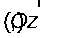
\includegraphics[width=\linewidth,height=.72\textheight,keepaspectratio]{images/image107.pdf} soit dirigé suivant la
  verticale descendante.
\item
  Le bras \textbf{1}, de repère associé
  \(R_{1}(O,\overset{\rightarrow}{x_{1}},\overset{\rightarrow}{y_{1}},\overset{\rightarrow}{z_{1}})\),
  en mouvement de rotation d'axe \((O,\overrightarrow{z})\) par rapport
  au bâti \textbf{0} tel que
  \(\overrightarrow{z} = \overrightarrow{z_{1}}\) et
  \(\alpha = (\overrightarrow{x},\overrightarrow{x_{1}})\).On pose
  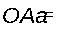
\includegraphics[width=\linewidth,height=.72\textheight,keepaspectratio]{images/image108.pdf}(a est une constante positive).
\item
  L a cabine \textbf{2}, de repère
  associé\(R_{2}(A,\overrightarrow{x_{2}},\overrightarrow{y_{2}},\overrightarrow{z_{2}})\),
  en mouvement de rotation d'axe \((A,\overrightarrow{y_{1}})\) par
  rapport au bras \textbf{1} tel que
  \(\overrightarrow{y_{1}} = \overrightarrow{y_{2}}\) et
  \((\overrightarrow{z_{1}},\overrightarrow{z_{2}}) = \beta\). Le centre
  de gravité G de la cabine \textbf{2} est tel que \(AG = b\) (b est une
  constante positive).
\end{itemize}

\textbf{Dessiner}, en indiquant sous chacune d'entre elles le vecteur
vitesse de rotation correspondant, les deux figures de changement de
base.

\textbf{Déterminer} le vecteur vitesse
\(\overrightarrow{V_{G \in 2/0}}\).

\textbf{Déterminer} le vecteur accélération
\(\overrightarrow{A_{G \in 2/0}}\).

\textbf{ROBOT MANIPULATEUR DEUX AXES}


\includegraphics[width=\linewidth,height=.72\textheight,keepaspectratio]{images/image101.png}
Niveau 1

Le robot manipulateur 2axes est représenté sous la forme du schéma
cinématique ci-dessous~:

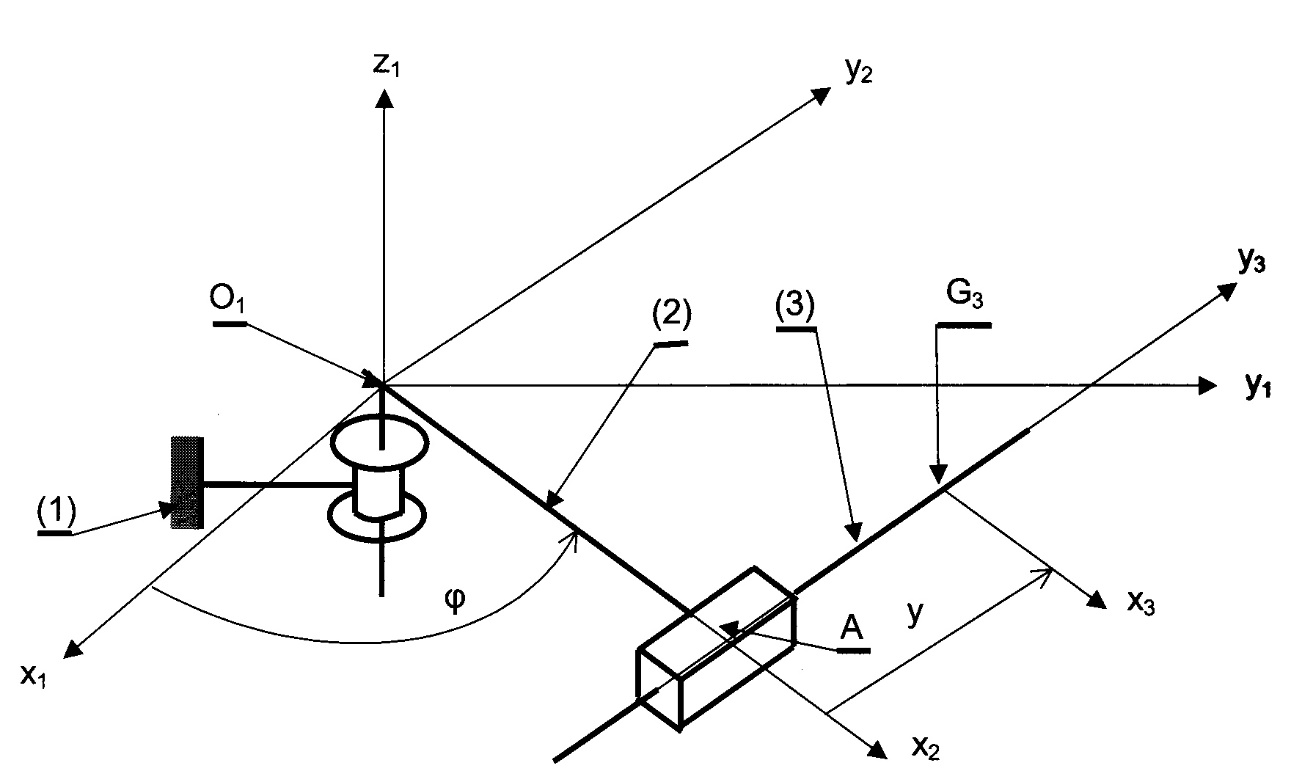
\includegraphics[width=\linewidth,height=.72\textheight,keepaspectratio]{images/image109.jpeg}

\textbf{\ul{Constituants et paramétrage~}}

\begin{itemize}
\item
  Le socle \textbf{1}, de repère associé
  \(R_{1}(O_{1},\overrightarrow{x_{1}},\overrightarrow{y_{1}},\overrightarrow{z_{1}})\),
  est fixe par rapport au sol tel que l'axe
  \((O_{1},{\overrightarrow{z}}_{1})\) soit dirigé suivant la verticale
  ascendante.
\item
  Le corps \textbf{2}, de repère associé
  \(R_{2}(O_{1},\overrightarrow{x_{2}},\overrightarrow{y_{2}},\overrightarrow{z_{2}})\),
  est en mouvement de rotation d'axe
  \((O_{1},{\overrightarrow{z}}_{1})\) par rapport au socle \textbf{1}
  tel que \(\overrightarrow{z_{1}} = \overrightarrow{z_{2}}\) et
  \(\phi = (\overrightarrow{x_{1}},\overrightarrow{x_{2}})\).On pose
  \(O_{1}A = a\) (a est une constante positive).
\item
  Le bras \textbf{3}, de repère
  associé\(R_{3}(G_{3},\overrightarrow{x_{3}},\overrightarrow{y_{3}},\overrightarrow{z_{3}})\),
  est en mouvement de translation rectiligne de direction
  \(\overrightarrow{y_{2}} = \overrightarrow{y_{3}}\) par rapport au
  corps \textbf{2} tel que
  \(\overrightarrow{AG_{3}} = y(t) \cdot \overrightarrow{y_{3}}\).
  G\textsubscript{3} est le centre de gravité du bras \textbf{3}.
\end{itemize}

\textbf{Dessiner}, en indiquant en dessous le vecteur vitesse de
rotation correspondant, la figure de changement de base.

\textbf{Déterminer} le vecteur vitesse
\(\overrightarrow{V_{G_{3} \in 3/1}}\).

\textbf{Déterminer} le vecteur accélération
\(\overrightarrow{A_{G_{3} \in 3/1}}\).

\textbf{\hfill\break
}

\textbf{TRANSPORTEUR HORIZONTAL}


\includegraphics[width=\linewidth,height=.72\textheight,keepaspectratio]{images/image101.png}
Niveau 1

Un mécanisme de transport de charge est constitué d'un rail fixe \ul{1},
d'un chariot mobile \ul{2} en liaison glissière avec ce dernier, d'un
bras rigide \ul{3} articulé en B sur le chariot. La charge est située en
C. Le mécanisme évolue dans le plan
\(\left( \text{O}_{\text{1}}\text{, }\overrightarrow{\text{x}_{\text{1}}}\text{, }\overrightarrow{\text{y}_{\text{1}}} \right)\)
vertical. Les liaisons sont parf. Le but de cet exercice est d'analyser
le mouvement du bras et donc de la charge lors des séquences
d'accélération et de mouvement uniforme du chariot.


\includegraphics[width=\linewidth,height=.72\textheight,keepaspectratio]{images/image110.jpeg}

Repère R\textsubscript{2} parallèle à R\textsubscript{1}. AB = h,
O\textsubscript{1}A = x(t)

G3~: centre d'inertie du bras et de la charge placée en C.
BG\textsubscript{3} = L\textsubscript{3}.

\textbf{\ul{Qu. 1}} Donner le torseur \(\left\{ V_{2/1} \right\}_{A}\).
Donner le torseur \(\left\{ V_{3/2} \right\}_{A}\).

\textbf{\ul{Qu. 2}} Déterminer l'expression des accélérations
suivantes~:

\begin{enumerate}
\def\labelenumi{(\alph{enumi})}
\item
  \(\overrightarrow{A_{A \in 2/R_{1}}}\) en fonction de
  \(\ddot{\text{x}}\)~;
\item
  \(\overrightarrow{A_{G_{3} \in 3/R_{1}}}\) en fonction de
  \(\ddot{\text{x}}\) \(\Gamma\), L\textsubscript{3}, \(\dot{\text{$\theta$}}\)
  et \(\ddot{\text{$\theta$}}\).
\end{enumerate}

\emph{\hfill\break
}


\includegraphics[width=\linewidth,height=.72\textheight,keepaspectratio]{images/image101.png}
Niveau 1


\includegraphics[width=\linewidth,height=.72\textheight,keepaspectratio]{images/image111.jpeg}
\textbf{CENTRE D'USINAGE 5 AXES À GRANDE VITESSE}

\emph{(\ul{Source~}: ATS 2006)}

\textbf{\ul{Objectif de l'étude~:}}

\begin{itemize}
\item
  \textbf{Exprimer} la vitesse de l'extrémité de l'outil dans son
  mouvement par rapport à la pièce en fonction des paramètres de
  mouvement proposés et des dimensions du système.
\end{itemize}

\begin{enumerate}
\item
  Mise en situation
\end{enumerate}


\includegraphics[width=\linewidth,height=.72\textheight,keepaspectratio]{images/image112.png}L'usinage,
opération de transformation d'un produit par enlèvement de matière, est
à la base de la fabrication de produits dans les industries mécaniques.
On appelle le moyen de production associé à une opération d'usinage une
machine-outil ou un centre d'usinage.

Outil

La génération d'une surface par enlèvement de matière est obtenue grâce
à un outil muni d'au moins une arête coupante. L'outil se déplace par
rapport à la pièce installée sur la machine-outil. C'est le mouvement
d'avance.

\emph{Figure 1~: Opération d'usinage de forme complexe}

Pièce

Le fraisage est un procédé d'usinage particulier dans lequel l'outil
doit en plus tourner sur lui-même par rapport au bâti de la
machine-outil pour pouvoir couper la matière. C'est le mouvement de
coupe.

Les contraintes d'accessibilité pour l'usinage de formes complexes
(figures 1 et 2) justifient l'utilisation de machines-outils spécifiques
capables~:

\begin{itemize}
\item
  de translater l'outil par rapport à la pièce dans 3 directions
  orthogonales~;
\item
  d'orienter l'axe de l'outil par rapport à la pièce autour de 2
  directions.
\end{itemize}


\includegraphics[width=\linewidth,height=.72\textheight,keepaspectratio]{images/image113.png}

\emph{Figure 2~: Exemple de pièce de forme complexe}

Un «~\textbf{axe}~» sur une machine-outil est un système qui gère l'un
des mouvements d'avance de l'outil par rapport à la pièce. Un
«~\textbf{axe}~» est composé d'une partie commande et d'une partie
opérative. Cette partie opérative est généralement constituée~:

\begin{itemize}
\item
  d'un modulateur d'énergie (c'est le préactionneur)
\item
  d'un moteur (c'est l'actionneur),
\item
  d'un mobile (c'est l'élément dont on veut commander le déplacement),
\item
  d'un système de transformation de mouvement entre le moteur et le
  mobile,
\item
  de capteurs (généralement un capteur de vitesse et un capteur de
  position).
\end{itemize}

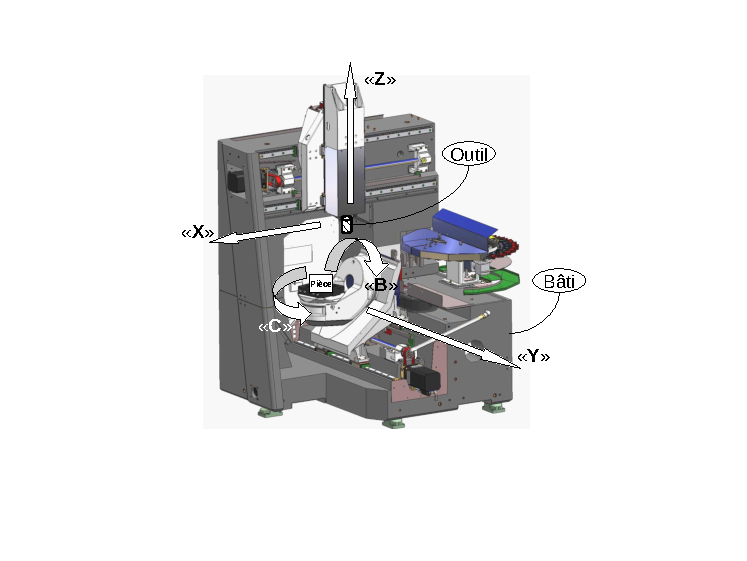
\includegraphics[width=\linewidth,height=.72\textheight,keepaspectratio]{images/image114.pdf}Le
centre d'usinage «~\textbf{5 axes}~» \textbf{HSM 600U} de la société
\textbf{Mikron,} représenté sur la figure 3, permet l'usinage de formes
complexes. Il est constitué d'un bâti supportant~:

\begin{itemize}
\item
  2 «~\textbf{axes~}» pour la mise en mouvement de l'outil par rapport
  au bâti. Ces 2 translations sont notées «~X~» et «~Z~».
\item
  3 «~\textbf{axes}~» pour la mise en mouvement de la pièce par rapport
  au bâti. Une troisième translation est notée «~Y~» et les 2 rotations
  sont notées «~B~» et «~C~».
\item
  un dispositif de mise en rotation de l'outil autour de son axe
  géométrique par rapport au bâti. Cette rotation génère le mouvement de
  coupe\emph{.}
\end{itemize}

\begin{quote}
\emph{Figure 3~: Vue globale du centre d'usinage avec repérage des
«~axes~»}
\end{quote}

\textbf{FAST descriptif partiel du centre d'usinage~«~5 axes~».}

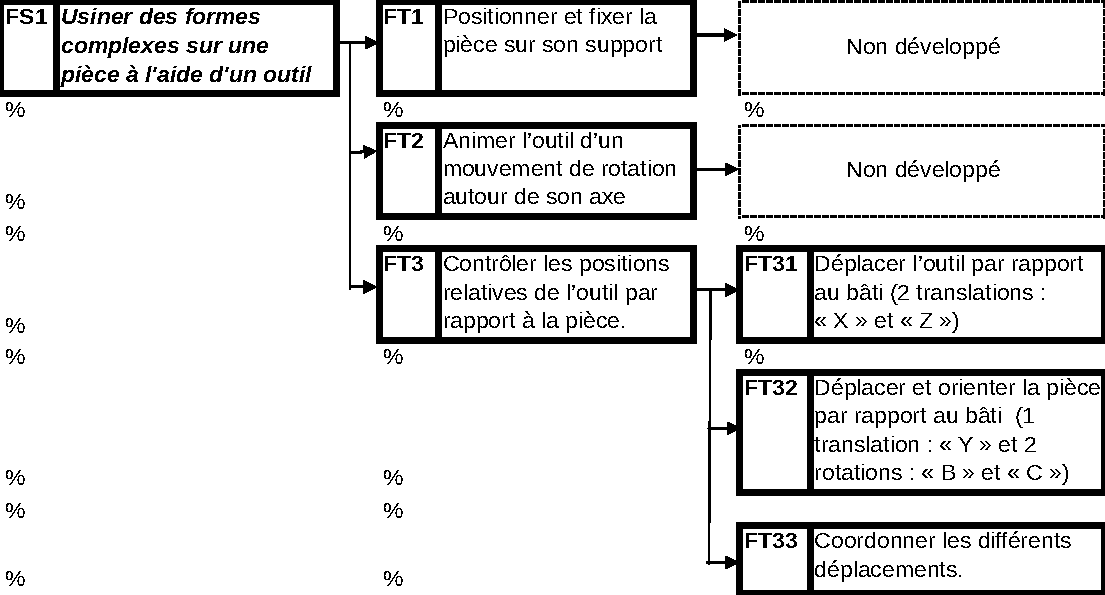
\includegraphics[width=\linewidth,height=.72\textheight,keepaspectratio]{images/image115.pdf}

\emph{\textbf{Performances des axes «~X~», «~Y~» et «~Z~» du centre
d'usinage.}}

\begin{longtable}{@{}
  >{\raggedright\arraybackslash}p{(\columnwidth - 8\tabcolsep) * \real{0.2838}}
  >{\raggedright\arraybackslash}p{(\columnwidth - 8\tabcolsep) * \real{0.1493}}
  >{\raggedright\arraybackslash}p{(\columnwidth - 8\tabcolsep) * \real{0.1494}}
  >{\raggedright\arraybackslash}p{(\columnwidth - 8\tabcolsep) * \real{0.2118}}
  >{\raggedright\arraybackslash}p{(\columnwidth - 8\tabcolsep) * \real{0.2057}}@{}}
\toprule\noalign{}
\endhead
\bottomrule\noalign{}
\endlastfoot
& \textbf{Variables} & \textbf{Course} & \textbf{Vitesse maximale} &
\textbf{Couple moteur} \\
Axe «~X~» (longitudinal) & \emph{x(t)} & 800 mm & 40 m/min & 42 Nm \\
Axe «~Y~» (transversal) & \emph{y(t)} & 600 mm & 40 m/min & \emph{Non
communiqué} \\
Axe «~Z~» (vertical) & \emph{z(t)} & 500 mm & 40 m/min & \emph{Non
communiqué} \\
\end{longtable}

\emph{\textbf{Performances des axes «~B~» et «~C~» du centre
d'usinage.}}

\begin{longtable}{@{}
  >{\raggedright\arraybackslash}p{(\columnwidth - 10\tabcolsep) * \real{0.2051}}
  >{\raggedright\arraybackslash}p{(\columnwidth - 10\tabcolsep) * \real{0.1657}}
  >{\raggedright\arraybackslash}p{(\columnwidth - 10\tabcolsep) * \real{0.1657}}
  >{\raggedright\arraybackslash}p{(\columnwidth - 10\tabcolsep) * \real{0.1759}}
  >{\raggedright\arraybackslash}p{(\columnwidth - 10\tabcolsep) * \real{0.1602}}
  >{\raggedright\arraybackslash}p{(\columnwidth - 10\tabcolsep) * \real{0.1273}}@{}}
\toprule\noalign{}
\endhead
\bottomrule\noalign{}
\endlastfoot
& \textbf{Variables} & \textbf{Course} & \textbf{Vitesse maximale} &
\textbf{Accélération angulaire} & \textbf{Couple moteur} \\
Axe «~B~» & \emph{$\alpha$ (t)} & + 30° / - 110° & 150 tours/min & 50
rd/s\textsuperscript{2} & 680 Nm \\
Axe «~C~» & \emph{$\beta$ (t)} & 360° & 250 tours/min & 100
rd/s\textsuperscript{2} & 340 Nm \\
\end{longtable}

\emph{\textbf{Schéma cinématique et paramétrage}}


\includegraphics[width=\linewidth,height=.72\textheight,keepaspectratio]{images/image49.png}

\emph{Figure 4~: schéma cinématique}

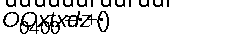
\includegraphics[width=\linewidth,height=.72\textheight,keepaspectratio]{images/image116.pdf}
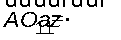
\includegraphics[width=\linewidth,height=.72\textheight,keepaspectratio]{images/image117.pdf}
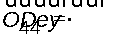
\includegraphics[width=\linewidth,height=.72\textheight,keepaspectratio]{images/image118.pdf}

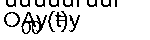
\includegraphics[width=\linewidth,height=.72\textheight,keepaspectratio]{images/image119.pdf}
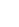
\includegraphics[width=\linewidth,height=.72\textheight,keepaspectratio]{images/image27.pdf}
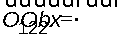
\includegraphics[width=\linewidth,height=.72\textheight,keepaspectratio]{images/image120.pdf}
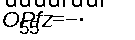
\includegraphics[width=\linewidth,height=.72\textheight,keepaspectratio]{images/image121.pdf}

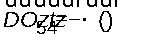
\includegraphics[width=\linewidth,height=.72\textheight,keepaspectratio]{images/image122.pdf}
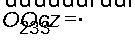
\includegraphics[width=\linewidth,height=.72\textheight,keepaspectratio]{images/image123.pdf}
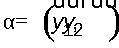
\includegraphics[width=\linewidth,height=.72\textheight,keepaspectratio]{images/image124.pdf}et
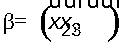
\includegraphics[width=\linewidth,height=.72\textheight,keepaspectratio]{images/image125.pdf}

Où 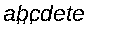
\includegraphics[width=\linewidth,height=.72\textheight,keepaspectratio]{images/image126.pdf} sont des constantes liées à
l'architecture de la machine.

\begin{longtable}{@{}
  >{\raggedright\arraybackslash}p{(\columnwidth - 6\tabcolsep) * \real{0.3837}}
  >{\raggedright\arraybackslash}p{(\columnwidth - 6\tabcolsep) * \real{0.1290}}
  >{\raggedright\arraybackslash}p{(\columnwidth - 6\tabcolsep) * \real{0.2006}}
  >{\raggedright\arraybackslash}p{(\columnwidth - 6\tabcolsep) * \real{0.2867}}@{}}
\toprule\noalign{}
\begin{minipage}[b]{\linewidth}\raggedright
\end{minipage} & \begin{minipage}[b]{\linewidth}\raggedright
\emph{\textbf{Masse}}
\end{minipage} & \begin{minipage}[b]{\linewidth}\raggedright
\emph{\textbf{Centre d'inertie}}
\end{minipage} & \begin{minipage}[b]{\linewidth}\raggedright
\emph{\textbf{Repères associés}}
\end{minipage} \\
\midrule\noalign{}
\endhead
\bottomrule\noalign{}
\endlastfoot
\emph{\textbf{Solide S3 (pièce usinée et son support)}} &
\emph{\textbf{M0}} & \emph{\textbf{G0}} &
\emph{\textbf{R\textsubscript{3}=}}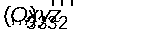
\includegraphics[width=\linewidth,height=.72\textheight,keepaspectratio]{images/image127.pdf} \\
\emph{\textbf{Solide S2}} & \emph{\textbf{M2}} & \emph{\textbf{G2}} &
\emph{\textbf{R\textsubscript{2}=}}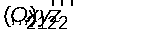
\includegraphics[width=\linewidth,height=.72\textheight,keepaspectratio]{images/image128.pdf} \\
\emph{\textbf{Solide S1}} & \emph{\textbf{M1}} & \emph{\textbf{G1}} &
\emph{\textbf{R\textsubscript{1}=}}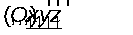
\includegraphics[width=\linewidth,height=.72\textheight,keepaspectratio]{images/image129.pdf} \\
\emph{\textbf{Solide S0 (le bâti de la machine)}} & \emph{\textbf{M3}} &
\emph{\textbf{G3}} &
\emph{\textbf{R\textsubscript{0}=}}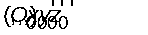
\includegraphics[width=\linewidth,height=.72\textheight,keepaspectratio]{images/image130.pdf} \\
\emph{\textbf{Solide S4}} & \emph{\textbf{M4}} & \emph{\textbf{G4}} &
\emph{\textbf{R\textsubscript{4}=}}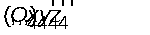
\includegraphics[width=\linewidth,height=.72\textheight,keepaspectratio]{images/image131.pdf} \\
\emph{\textbf{Solide S5}} & \emph{\textbf{M5}} & \emph{\textbf{G5}} &
\emph{\textbf{R\textsubscript{5}=}}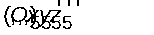
\includegraphics[width=\linewidth,height=.72\textheight,keepaspectratio]{images/image132.pdf} \\
\end{longtable}

\begin{enumerate}
\item
  Etude préliminaire
\end{enumerate}

\textbf{Q1.} Indiquer la nature du mouvement du solide 1 par rapport au
solide 0.

\textbf{Q2.} Indiquer la nature du mouvement du solide 4 par rapport au
solide 0.

\textbf{Q3.} Indiquer la nature du mouvement du solide 5 par rapport au
solide 4.

\textbf{Q4.} En déduire la relation entre les bases des repères
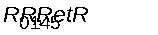
\includegraphics[width=\linewidth,height=.72\textheight,keepaspectratio]{images/image133.pdf} .

\textbf{Q5.} Indiquer la nature du mouvement du solide 2 par rapport au
solide 1.

\textbf{Q6.} Dessiner la figure de changement de base correspondant à ce
mouvement.

\textbf{Q7.} Indiquer la nature du mouvement du solide 3 par rapport au
solide 2.

\textbf{Q8.} Dessiner la figure de changement de base correspondant à ce
mouvement.

\begin{enumerate}
\setcounter{enumi}{1}
\item
  Comportement cinématique
\end{enumerate}

\textbf{Q9.} Exprimer le vecteur position
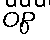
\includegraphics[width=\linewidth,height=.72\textheight,keepaspectratio]{images/image134.pdf} dans la base du référentiel
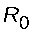
\includegraphics[width=\linewidth,height=.72\textheight,keepaspectratio]{images/image135.pdf}.

N.B~: Le point 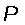
\includegraphics[width=\linewidth,height=.72\textheight,keepaspectratio]{images/image136.pdf} est situé sur
l'axe de rotation de l'outil par rapport au solide 5, il est donc fixe
par rapport à 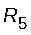
\includegraphics[width=\linewidth,height=.72\textheight,keepaspectratio]{images/image137.pdf}\textbf{.}

\textbf{Q10.} Déterminer le vecteur vitesse du point
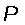
\includegraphics[width=\linewidth,height=.72\textheight,keepaspectratio]{images/image138.pdf}appartenant à l'outil, dans son
mouvement par rapport à~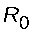
\includegraphics[width=\linewidth,height=.72\textheight,keepaspectratio]{images/image139.pdf}. Cette
vitesse sera notée~: 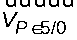
\includegraphics[width=\linewidth,height=.72\textheight,keepaspectratio]{images/image140.pdf}

\textbf{Q11.} En déduire la vitesse maximale du point
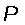
\includegraphics[width=\linewidth,height=.72\textheight,keepaspectratio]{images/image141.pdf}appartenant à l'outil, dans son
mouvement par rapport à~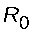
\includegraphics[width=\linewidth,height=.72\textheight,keepaspectratio]{images/image142.pdf}.

\textbf{Q12.} Exprimer le vecteur position
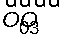
\includegraphics[width=\linewidth,height=.72\textheight,keepaspectratio]{images/image143.pdf} dans les bases des référentiels
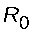
\includegraphics[width=\linewidth,height=.72\textheight,keepaspectratio]{images/image144.pdf} et
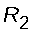
\includegraphics[width=\linewidth,height=.72\textheight,keepaspectratio]{images/image145.pdf} .

\textbf{Q13.} Déterminer le vecteur vitesse du point
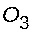
\includegraphics[width=\linewidth,height=.72\textheight,keepaspectratio]{images/image70.pdf} appartenant au solide 3 (pièce
usinée + support), dans son mouvement par rapport
à~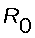
\includegraphics[width=\linewidth,height=.72\textheight,keepaspectratio]{images/image146.pdf}. Cette vitesse sera notée~:
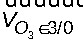
\includegraphics[width=\linewidth,height=.72\textheight,keepaspectratio]{images/image147.pdf}.

\textbf{Q14.} Déterminer le vecteur accélération du point
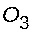
\includegraphics[width=\linewidth,height=.72\textheight,keepaspectratio]{images/image70.pdf}appartenant au solide 3, dans son
mouvement par rapport à~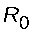
\includegraphics[width=\linewidth,height=.72\textheight,keepaspectratio]{images/image148.pdf}. Cette
accélération sera notée~: 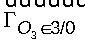
\includegraphics[width=\linewidth,height=.72\textheight,keepaspectratio]{images/image149.pdf}

\textbf{Q15.} Déterminer le vecteur rotation
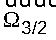
\includegraphics[width=\linewidth,height=.72\textheight,keepaspectratio]{images/image150.pdf}.

\textbf{Q16.} En déduire le vecteur rotation
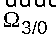
\includegraphics[width=\linewidth,height=.72\textheight,keepaspectratio]{images/image151.pdf}.

\textbf{Q17.} Retrouver le résultat de la question \textbf{Q13.} en
utilisant la relation de composition des vecteurs vitesse et la relation
du champ des vecteurs vitesse.

La surface usinée est définie comme un ensemble de points
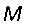
\includegraphics[width=\linewidth,height=.72\textheight,keepaspectratio]{images/image152.pdf} de coordonnées
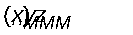
\includegraphics[width=\linewidth,height=.72\textheight,keepaspectratio]{images/image153.pdf}dans le repère
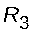
\includegraphics[width=\linewidth,height=.72\textheight,keepaspectratio]{images/image154.pdf}.

On note 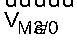
\includegraphics[width=\linewidth,height=.72\textheight,keepaspectratio]{images/image155.pdf} le vecteur vitesse du
point 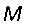
\includegraphics[width=\linewidth,height=.72\textheight,keepaspectratio]{images/image156.pdf} appartenant \emph{au solide
3}, dans son mouvement par rapport à
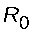
\includegraphics[width=\linewidth,height=.72\textheight,keepaspectratio]{images/image157.pdf}.

\emph{\textbf{Q18.} Donner la relation entre les
vecteurs}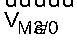
\includegraphics[width=\linewidth,height=.72\textheight,keepaspectratio]{images/image155.pdf}\emph{,}
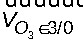
\includegraphics[width=\linewidth,height=.72\textheight,keepaspectratio]{images/image147.pdf} \emph{et}
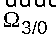
\includegraphics[width=\linewidth,height=.72\textheight,keepaspectratio]{images/image151.pdf}\emph{.}

\emph{\textbf{Q19.} Déterminer le vecteur vitesse}
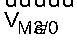
\includegraphics[width=\linewidth,height=.72\textheight,keepaspectratio]{images/image155.pdf} \emph{dans le cas ou}
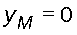
\includegraphics[width=\linewidth,height=.72\textheight,keepaspectratio]{images/image158.pdf} (point
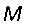
\includegraphics[width=\linewidth,height=.72\textheight,keepaspectratio]{images/image159.pdf}situé dans le plan
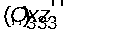
\includegraphics[width=\linewidth,height=.72\textheight,keepaspectratio]{images/image160.pdf})

On note 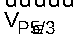
\includegraphics[width=\linewidth,height=.72\textheight,keepaspectratio]{images/image161.pdf} le vecteur vitesse du
point 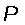
\includegraphics[width=\linewidth,height=.72\textheight,keepaspectratio]{images/image162.pdf} situé à l'extrémité de
l'outil, dans son mouvement par rapport à
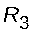
\includegraphics[width=\linewidth,height=.72\textheight,keepaspectratio]{images/image163.pdf}, le repère lié à la pièce usinée.

\emph{\textbf{Q20.} Donner la relation entre les
vecteurs}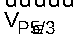
\includegraphics[width=\linewidth,height=.72\textheight,keepaspectratio]{images/image164.pdf}\emph{,}
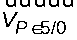
\includegraphics[width=\linewidth,height=.72\textheight,keepaspectratio]{images/image165.pdf} \emph{et}
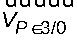
\includegraphics[width=\linewidth,height=.72\textheight,keepaspectratio]{images/image166.pdf}\emph{.}

\emph{\textbf{Q21.} En déduire une relation entre les
vecteurs}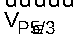
\includegraphics[width=\linewidth,height=.72\textheight,keepaspectratio]{images/image164.pdf}\emph{,}
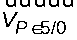
\includegraphics[width=\linewidth,height=.72\textheight,keepaspectratio]{images/image165.pdf}\emph{,}
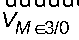
\includegraphics[width=\linewidth,height=.72\textheight,keepaspectratio]{images/image167.pdf}\emph{et}
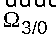
\includegraphics[width=\linewidth,height=.72\textheight,keepaspectratio]{images/image151.pdf}\emph{.}

\emph{Lors de l'usinage, Le point}
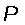
\includegraphics[width=\linewidth,height=.72\textheight,keepaspectratio]{images/image162.pdf} \emph{doit se déplacer sur la
surface usinée définie comme le lieu des points}
\includegraphics[width=\linewidth,height=.72\textheight,keepaspectratio]{images/image168.pdf}
\emph{(}\includegraphics[width=\linewidth,height=.72\textheight,keepaspectratio]{images/image162.pdf} \emph{confondu avec}
\includegraphics[width=\linewidth,height=.72\textheight,keepaspectratio]{images/image168.pdf}\emph{).}

\emph{\textbf{Q22.} Que devient alors la relation obtenue à la question
\textbf{Q21~}?}

\emph{\hfill\break
}

\includegraphics[width=\linewidth,height=.72\textheight,keepaspectratio]{images/image169.png}\textbf{ECHELLE
EPAS}

\includegraphics[width=\linewidth,height=.72\textheight,keepaspectratio]{images/image101.png}
Niveau 1

\includegraphics[width=\linewidth,height=.72\textheight,keepaspectratio]{images/image101.png}
Niveau 1

\emph{(\ul{Source :} Centrale Supélec PSI 2007)}

\textbf{\ul{Objectif de l'étude~:}}

\begin{itemize}
\item
  \textbf{Déterminer}, dans le but de valider le critère du Cahier des
  Charges Fonctionnel, le vecteur accélération du
  point\includegraphics[width=\linewidth,height=.72\textheight,keepaspectratio]{images/image170.pdf} appartenant à l'échelle
  dans son mouvement par rapport au~sol (lors d'une phase de dressage de
  l'échelle).

  \begin{enumerate}
  \item
    Mise en situation
  \end{enumerate}
\end{itemize}

\includegraphics[width=\linewidth,height=.72\textheight,keepaspectratio]{images/image171.png}

On s'intéresse à une Echelle Pivotante Automatique à commande
Séquentielle. Ce système conçu et commercialisé par la société CAMIVA
est monté sur le châssis d'un camion de pompiers et permet de déplacer
une plate-forme pouvant recevoir deux personnes et un brancard (charge
maxi 270 kg) le plus rapidement possible et en toute sécurité.

Le système est représenté sous forme de schéma cinématique ci-dessous~:

\includegraphics[width=\linewidth,height=.72\textheight,keepaspectratio]{images/image172.png}

Ce système est constitué de cinq solides~:

\begin{itemize}
\item
  Le châssis \textbf{0}, de repère associé
  \includegraphics[width=\linewidth,height=.72\textheight,keepaspectratio]{images/image173.pdf}, fixe par rapport au sol tel
  que l'axe \includegraphics[width=\linewidth,height=.72\textheight,keepaspectratio]{images/image174.pdf} soit dirigé suivant
  la verticale ascendante.
\item
  La tourelle \textbf{1}, de repère associé
  \includegraphics[width=\linewidth,height=.72\textheight,keepaspectratio]{images/image175.pdf}, en mouvement de rotation (non
  étudié ici) d'axe \includegraphics[width=\linewidth,height=.72\textheight,keepaspectratio]{images/image176.pdf} par rapport
  au mât \textbf{0} tel que \includegraphics[width=\linewidth,height=.72\textheight,keepaspectratio]{images/image177.pdf}.
\item
  Le berceau \textbf{2}, de repère associé
  \includegraphics[width=\linewidth,height=.72\textheight,keepaspectratio]{images/image178.pdf}, en mouvement de rotation d'axe
  \includegraphics[width=\linewidth,height=.72\textheight,keepaspectratio]{images/image179.pdf} par rapport à la tourelle
  \textbf{1} tel que \includegraphics[width=\linewidth,height=.72\textheight,keepaspectratio]{images/image180.pdf} (a et
  \emph{b} constants), \includegraphics[width=\linewidth,height=.72\textheight,keepaspectratio]{images/image181.pdf}
  (c~constant), \includegraphics[width=\linewidth,height=.72\textheight,keepaspectratio]{images/image182.pdf} et
  \includegraphics[width=\linewidth,height=.72\textheight,keepaspectratio]{images/image183.pdf}.
\item
  L'échelle \textbf{3}, de repère
  associé\includegraphics[width=\linewidth,height=.72\textheight,keepaspectratio]{images/image184.pdf}, en mouvement de
  translation rectiligne de direction
  \includegraphics[width=\linewidth,height=.72\textheight,keepaspectratio]{images/image185.pdf} par rapport au berceau
  \textbf{2} tel que \includegraphics[width=\linewidth,height=.72\textheight,keepaspectratio]{images/image186.pdf}.
\item
  Le vérin de dressage \textbf{4} + \textbf{5} (non étudié
  ici)\textbf{.}
\end{itemize}

Pour des raisons de confort et de sécurité, il est nécessaire que
pendant la phase de dressage* de l'échelle, la norme de l'accélération
subie par une personne située dans la nacelle ne dépassement un niveau
défini dans le CdCF.

\emph{*\ul{Phase de dressage~:} les vérins de dressage font pivoter le
berceau \textbf{2} pendant que le parc échelle \textbf{3} se déploie.
Pendant cette phase, le système d'orientation de la tourelle \textbf{1}
est inactif~(}\includegraphics[width=\linewidth,height=.72\textheight,keepaspectratio]{images/image187.pdf})\emph{.}

\textbf{Q1.} Donner la nature des mouvements Mvt 2/0, Mvt 3/2 et Mvt
3/0.

\textbf{Q2.} En déduire les trajectoires
\protect\includegraphics[width=\linewidth,height=.72\textheight,keepaspectratio]{images/image188.pdf},\protect\includegraphics[width=\linewidth,height=.72\textheight,keepaspectratio]{images/image189.pdf}
et \protect\includegraphics[width=\linewidth,height=.72\textheight,keepaspectratio]{images/image190.pdf} .

\emph{\textbf{Q3.} Que peut-on dire sur les bases des repères}
\includegraphics[width=\linewidth,height=.72\textheight,keepaspectratio]{images/image191.pdf}\emph{~? En déduire}
\includegraphics[width=\linewidth,height=.72\textheight,keepaspectratio]{images/image192.pdf}

\textbf{Q4.} Dessiner la figure de changement de base correspondant au
mouvement entre \textbf{2} et \textbf{1} .

\textbf{Q5.} Indiquer sous cette figure l'expression du vecteur rotation
correspondant.

\textbf{Q6.} En déduire l'expression de
\protect\includegraphics[width=\linewidth,height=.72\textheight,keepaspectratio]{images/image193.pdf}.

\textbf{Q7.} Déterminer le vecteur vitesse
\protect\includegraphics[width=\linewidth,height=.72\textheight,keepaspectratio]{images/image194.pdf}.

\textbf{Q8.} Déterminer le vecteur accélération
\protect\includegraphics[width=\linewidth,height=.72\textheight,keepaspectratio]{images/image195.pdf}.

\textbf{\ul{\hfill\break
}}

\includegraphics[width=\linewidth,height=.72\textheight,keepaspectratio]{images/image196.pdf}\textbf{MANIPULATEUR DE STÈLES DE
MARBRE}

\includegraphics[width=\linewidth,height=.72\textheight,keepaspectratio]{images/image101.png}
Niveau 1

\emph{(\ul{Source} : Jacques Le Goff)}

\textbf{\ul{Objectif de l'étude~:}}

\begin{itemize}
\item
  \textbf{Déterminer} le vecteur accélération d'un point de la stèle par
  rapport au repère fixe R0 dans le cas d'une combinaison des mouvements
  d'élévation et d'inclinaison.

  \begin{enumerate}
  \item
    Mise en situation
  \end{enumerate}
\end{itemize}

\includegraphics[width=\linewidth,height=.72\textheight,keepaspectratio]{images/image197.pdf}La société FERGEAU implantée en
Bretagne, développe depuis des années des biens d'équipement relatifs à
l'industrie granitière.

Pour satisfaire les besoins de sa clientèle, FERGEAU propose une
meuleuse hydraulique portative accompagnée d'accessoires dont un
manipulateur de stèles, objet de l'étude.

Les stèles sont des plaques de marbre ou de granit (de 6 à 10 cm
d'épaisseur et pouvant atteindre la masse de 400 kg), destinées à
recevoir des textes et des motifs ornementaux réalisés par abrasion.

Les chants de cette pierre sont polis à l'aide de la meuleuse
hydraulique portative, le manipulateur a donc pour fonction~:

\begin{itemize}
\item
  de déplacer et positionner la stèle par rapport à l'opérateur, pour
  lui faciliter les opérations à réaliser,
\item
  de maintenir la stèle en toute sécurité dans la position choisie,
  pendant le travail.
\end{itemize}

Ce produit est réalisé à raison d'une moyenne de 10 unités par an.

Trois déplacements indépendants peuvent être donnés à la pierre~:

\begin{itemize}
\item
  élévation et inclinaison réalisées à l'aide de deux vérins
  hydrauliques,
\item
  orientation réalisée manuellement.
\end{itemize}

Une étude préalable (AMDEC Produit) a permis de mettre en évidence les
risques potentiels les plus graves, de nature à compromettre la sécurité
de l'utilisateur.

\includegraphics[width=\linewidth,height=.72\textheight,keepaspectratio]{images/image198.png}

\includegraphics[width=\linewidth,height=.72\textheight,keepaspectratio]{images/image199.png}

\includegraphics[width=\linewidth,height=.72\textheight,keepaspectratio]{images/image200.png}

\textbf{\ul{Schéma cinématique du manipulateur de stèles de marbre}}

O\textsubscript{3}

O\textsubscript{6}

H

$\theta$

\emph{Les dimensions du système sont à lire sur la figure 3}

\includegraphics[width=\linewidth,height=.72\textheight,keepaspectratio]{images/image202.pdf}

\includegraphics[width=\linewidth,height=.72\textheight,keepaspectratio]{images/image202.pdf}

\includegraphics[width=\linewidth,height=.72\textheight,keepaspectratio]{images/image203.pdf}

\emph{\ul{Paramétrage~:}}

\includegraphics[width=\linewidth,height=.72\textheight,keepaspectratio]{images/image204.pdf}

J

\includegraphics[width=\linewidth,height=.72\textheight,keepaspectratio]{images/image206.png}\includegraphics[width=\linewidth,height=.72\textheight,keepaspectratio]{images/image207.png}

\begin{enumerate}
\item
  Comportement cinématique
\end{enumerate}

\begin{enumerate}
\def\labelenumi{\arabic{enumi}.}
\item
  Déterminer, de deux manières différentes (dérivée du vecteur position
  et composition des vitesses) le vecteur vitesse du point
  O\textsubscript{8} dans son mouvement par rapport au repère fixe
  R\textsubscript{0}. (on se placera dans le cas d'un mouvement combiné
  d'élévation et d'inclinaison) .
\item
  Déterminer, le vecteur accélération du point O\textsubscript{8} dans
  son mouvement par rapport au repère fixe R\textsubscript{0}. (on se
  placera dans le cas d'un mouvement combiné d'élévation et
  d'inclinaison).
\end{enumerate}

\includegraphics[width=\linewidth,height=.72\textheight,keepaspectratio]{images/image208.jpeg}\textbf{ROBOT
DE MANUTENTION}

\includegraphics[width=\linewidth,height=.72\textheight,keepaspectratio]{images/image101.png}
Niveau 1

\textbf{\ul{Objectif de l'étude~:}}

\begin{itemize}
\item
  \textbf{Déterminer} le vecteur vitesse d'un point du robot par rapport
  au repère fixe R0.

  \begin{enumerate}
  \item
    Mise en situation
  \end{enumerate}
\end{itemize}

Le système étudié (cf. figures) est un robot industriel destiné à la
manutention de pièces lourdes. Ce robot a une structure en
parallélogramme déformable qui lui permet de déplacer son poignet dans
l'aire de travail.

On associe à chaque solide i une base orthonormée directe
\includegraphics[width=\linewidth,height=.72\textheight,keepaspectratio]{images/image209.pdf}

Le mouvement de 1/0 est une rotation d'axe
\includegraphics[width=\linewidth,height=.72\textheight,keepaspectratio]{images/image210.pdf}~; on pose
\includegraphics[width=\linewidth,height=.72\textheight,keepaspectratio]{images/image211.pdf}

Le mouvement de 2/0 est une rotation d'axe
\includegraphics[width=\linewidth,height=.72\textheight,keepaspectratio]{images/image212.pdf}~; on pose
\includegraphics[width=\linewidth,height=.72\textheight,keepaspectratio]{images/image213.pdf}

Le mouvement de 1/3 est une rotation d'axe
\includegraphics[width=\linewidth,height=.72\textheight,keepaspectratio]{images/image214.pdf}~

Le mouvement de 2/4 est une rotation d'axe
\includegraphics[width=\linewidth,height=.72\textheight,keepaspectratio]{images/image215.pdf}~

Le mouvement de 3/4 est une rotation d'axe
\includegraphics[width=\linewidth,height=.72\textheight,keepaspectratio]{images/image216.pdf}~

Par ailleurs~: \includegraphics[width=\linewidth,height=.72\textheight,keepaspectratio]{images/image217.pdf},
\includegraphics[width=\linewidth,height=.72\textheight,keepaspectratio]{images/image218.pdf},\includegraphics[width=\linewidth,height=.72\textheight,keepaspectratio]{images/image219.pdf},\includegraphics[width=\linewidth,height=.72\textheight,keepaspectratio]{images/image220.pdf}et\includegraphics[width=\linewidth,height=.72\textheight,keepaspectratio]{images/image221.pdf}

\includegraphics[width=\linewidth,height=.72\textheight,keepaspectratio]{images/image222.png}\includegraphics[width=\linewidth,height=.72\textheight,keepaspectratio]{images/image223.jpeg}

\emph{figure 2}

\emph{figure 1}

Les mouvements du robot sont commandés par 2 moteurs~:

\begin{itemize}
\item
  Le solide 1 a son mouvement de rotation commandé par un moteur M1 tel
  que~: \includegraphics[width=\linewidth,height=.72\textheight,keepaspectratio]{images/image224.pdf}.
\item
  Le solide 2 a son mouvement de rotation commandé par un moteur M2 tel
  que~: \includegraphics[width=\linewidth,height=.72\textheight,keepaspectratio]{images/image225.pdf}

  \begin{enumerate}
  \item
    Comportement cinématique
  \end{enumerate}
\end{itemize}

\textbf{Q1.}Que peut-on dire sur les bases B\textsubscript{1},
B\textsubscript{2}, B\textsubscript{3} et B\textsubscript{4}~? En
déduire les 2 figures de changement de base définissant les 2 paramètres
d'orientation.

\textbf{Q2}. Déterminer les torseurs cinématiques
\protect\includegraphics[width=\linewidth,height=.72\textheight,keepaspectratio]{images/image226.pdf}
et\protect\includegraphics[width=\linewidth,height=.72\textheight,keepaspectratio]{images/image227.pdf}.

\textbf{Q3.} En déduire le torseur cinématique
\protect\includegraphics[width=\linewidth,height=.72\textheight,keepaspectratio]{images/image228.pdf}.

\textbf{Q4}. Déterminer les torseurs cinématiques
\protect\includegraphics[width=\linewidth,height=.72\textheight,keepaspectratio]{images/image229.pdf}
et\protect\includegraphics[width=\linewidth,height=.72\textheight,keepaspectratio]{images/image230.pdf}.

\textbf{Q5.} En déduire le torseur cinématique
\protect\includegraphics[width=\linewidth,height=.72\textheight,keepaspectratio]{images/image231.pdf}.

\textbf{Q6.} Déterminer le vecteur vitesse
\protect\includegraphics[width=\linewidth,height=.72\textheight,keepaspectratio]{images/image232.pdf}, en utilisant la relation
de composition des vitesses et la relation du champ des vecteurs vitesse
d'un solide.

\textbf{Q7.} Déterminer la trajectoire
\protect\includegraphics[width=\linewidth,height=.72\textheight,keepaspectratio]{images/image233.pdf} lorsque le moteur M2 est
à l'arrêt et \protect\includegraphics[width=\linewidth,height=.72\textheight,keepaspectratio]{images/image234.pdf}.

\textbf{Q8.} Déterminer la trajectoire
\protect\includegraphics[width=\linewidth,height=.72\textheight,keepaspectratio]{images/image235.pdf} lorsque le moteur M1 est
à l'arrêt et \protect\includegraphics[width=\linewidth,height=.72\textheight,keepaspectratio]{images/image236.pdf}.

\textbf{\ul{\hfill\break
}}

\includegraphics[width=\linewidth,height=.72\textheight,keepaspectratio]{images/image237.jpeg}\textbf{Monte-charge}

\includegraphics[width=\linewidth,height=.72\textheight,keepaspectratio]{images/image101.png}
Niveau 1

\emph{(\ul{Source : Jacques Le Goff})}

\textbf{\ul{Objectif de l'étude~:}}

\begin{quote}
A chaque phase, après avoir déterminité lés équations horaires du
mouvement, \textbf{tracer} l'évolution de la vitesse de rotation du
rotor du moteur en fonction du temps.
\end{quote}

\begin{itemize}
\item
  \begin{enumerate}
  \item
    \includegraphics[width=\linewidth,height=.72\textheight,keepaspectratio]{images/image238.png}
  \end{enumerate}
\end{itemize}

Le système de levage automatisé ci-contre permet de soulever une charge
par l'intermédiaire d'un système poulie + câble actionné par un moteur
électrique.

Des capteurs optiques permettent de détecter le passage de la charge
lors de sa montée et ainsi de donner l'ordre au moteur d'accélérer ou de
freiner.

\textbf{Le diamètre des poulies à été choisi afin que la charge monte de
10cm lorsque le moteur fait un tour.}

L'étude porte sur le mouvement de rotation du rotor du moteur décrit
ci-dessous~:

\ul{Description du cycle de levage~:}

- \emph{\ul{Première phase~:}} Le moteur se met en mouvement et accélère
(accélération constante) jusqu'à ce que la charge passe devant un
capteur situé à 0,5 m du sol.

- \emph{\ul{Deuxième phase~:}} puis il rejoint à la vitesse constante de
0,2 m/s le capteur situé à 1,5 m du sol.

- \emph{\ul{Troisième phase~:}} Une fois passé devant ce capteur, il
freine jusqu\textquotesingle à venir s'arrêter. La durée totale de
montée de la charge est alors de 15 secondes.

\begin{enumerate}
\setcounter{enumi}{1}
\item
  Travail demandé
\end{enumerate}

\begin{enumerate}
\def\labelenumi{\arabic{enumi}.}
\item
  \textbf{Déterminer} pour la première phase~: la nature du mouvement,
  l'accélération angulaire du moteur, et les équations horaires du
  mouvement du moteur.
\item
  \textbf{En déduire} la durée de cette phase de démarrage.
\item
  Après avoir déterminé parfaitement les équations du mouvement du
  moteur de la deuxième phase, \textbf{déterminer} la durée de
  fonctionnement du moteur (depuis sa mise en route) au moment il
  commence à freiner.
\item
  \textbf{Déterminer} la distance totale de montée de la charge (en
  mètre).
\end{enumerate}

\includegraphics[width=\linewidth,height=.72\textheight,keepaspectratio]{images/image101.png}
Niveau 4

\includegraphics[width=\linewidth,height=.72\textheight,keepaspectratio]{images/image239.jpeg}\textbf{ROBOT
DE SOUDAGE}

\emph{(\ul{Source : Jacques Le Goff})}

\textbf{\ul{Objectif de l'étude~:}}

\begin{itemize}
\item
  \textbf{Déterminer} la commandes des «~axes~» afin de réaliser un
  cordon se soudure linéaire de direction
  \includegraphics[width=\linewidth,height=.72\textheight,keepaspectratio]{images/image240.pdf}et lors du dégagement de
  l'organe terminal.

  \begin{enumerate}
  \item
    \includegraphics[width=\linewidth,height=.72\textheight,keepaspectratio]{images/image239.jpeg}Mise
    en situation
  \end{enumerate}
\end{itemize}

L\textquotesingle étude suivante porte sur un robot de soudure «~4
axes~» dont une modélisation cinématique est proposée sur \textbf{la
figure 1}.

Le robot est supposé constitué de quatre solides articulés entre eux, le
premier solide étant articulé sur un solide fixe S0.

\includegraphics[width=\linewidth,height=.72\textheight,keepaspectratio]{images/image241.png}
Chaque «~axe~» possède son propre actionneur, le mouvement entre solides
qui lui est associé peut donc être réalisé indépendamment des autres.

\textbf{Figure 1}~: modélisation cinématique du robot de soudage

Les repères liés à chaque solide ainsi que le paramétrage associé sont
définis ainsi~:

\includegraphics[width=\linewidth,height=.72\textheight,keepaspectratio]{images/image242.png}

\begin{enumerate}
\def\labelenumi{\arabic{enumi}.}
\item
  \textbf{Déterminer} la vitesse \includegraphics[width=\linewidth,height=.72\textheight,keepaspectratio]{images/image243.pdf}.
\item
  \textbf{Déterminer} la vitesse \includegraphics[width=\linewidth,height=.72\textheight,keepaspectratio]{images/image244.pdf}.
\item
  \textbf{Donner} le torseur cinématique, exprimé au point
  O\textsubscript{2}, du solide 2 dans son mouvement par rapport à
  R\textsubscript{0}.
\item
  \textbf{Déterminer} la vitesse \includegraphics[width=\linewidth,height=.72\textheight,keepaspectratio]{images/image245.pdf}.
\end{enumerate}

On souhaite réaliser un cordon de soudure linéaire de direction
\includegraphics[width=\linewidth,height=.72\textheight,keepaspectratio]{images/image246.pdf}. Il est nécessaire, pour que le
cordon de soudure soit correctement réalisé, que
\includegraphics[width=\linewidth,height=.72\textheight,keepaspectratio]{images/image247.pdf} (Moteur M1 bloqué),
\includegraphics[width=\linewidth,height=.72\textheight,keepaspectratio]{images/image248.pdf} et que
\includegraphics[width=\linewidth,height=.72\textheight,keepaspectratio]{images/image249.pdf} avec
\includegraphics[width=\linewidth,height=.72\textheight,keepaspectratio]{images/image250.pdf}.

\begin{enumerate}
\def\labelenumi{\arabic{enumi}.}
\setcounter{enumi}{4}
\item
  \textbf{Déterminer} les relations que doivent vérifier les paramètres
  de mouvement et leurs dérivées.
\end{enumerate}

Après la fin de l'opération de soudage, le robot effectue un dégagement
rapide du solide 4 afin de permettre l'enlèvement de la pièce soudée et
l'arrivée d'une nouvelle pièce à souder (Moteurs M1 et vérin V4 à
vitesse et accélération maximale).

Lors de cette phase, les moteurs M2 et M3 sont bloqués afin de maintenir
le solide 2 en positon verticale et le solide 3 en position horizontale
: \includegraphics[width=\linewidth,height=.72\textheight,keepaspectratio]{images/image251.pdf}et
\includegraphics[width=\linewidth,height=.72\textheight,keepaspectratio]{images/image252.pdf}

\begin{enumerate}
\def\labelenumi{\arabic{enumi}.}
\setcounter{enumi}{5}
\item
  \textbf{Déterminer} l'accélération
  \includegraphics[width=\linewidth,height=.72\textheight,keepaspectratio]{images/image253.pdf}.
\end{enumerate}

\textbf{\hfill\break
}

\includegraphics[width=\linewidth,height=.72\textheight,keepaspectratio]{images/image101.png}
Niveau 1

\includegraphics[width=\linewidth,height=.72\textheight,keepaspectratio]{images/image254.jpeg}\includegraphics[width=\linewidth,height=.72\textheight,keepaspectratio]{images/image255.jpeg}

\textbf{Scénic vs Ferrari F1}

\emph{(\ul{Source :})}

\textbf{\ul{Objectif de l'étude~:}}

\begin{itemize}
\item
  \textbf{Donner} les caractéristiques (a(t)~;v(t)~;x(t)) du mouvement
  de la voiture pour chaque phase dans le cas d'une formule 1 et d'un
  scenic 1,4 RTE.

  \begin{enumerate}
  \item
    Mise en situation
  \end{enumerate}
\end{itemize}

Une voiture se déplace en réalisant un mouvement de translation
rectiligne uniformément varié. Donner les caractéristiques
(a(t)~;v(t)~;x(t)) du mouvement de la voiture pour chaque phase dans le
cas d'une formule 1 et d'un scenic 1,4 RTE. Le mouvement est composé de
trois phases~: \textsc{Accélération jusqu\textquotesingle à 100km/h, 10
secondes à 100km/h, freinage jusqu\textquotesingle à l'arrêt.}

t\textsubscript{1}

t\textsubscript{2}

t\textsubscript{3}

100 km/h

\textbf{v\textsubscript{(t)}}

\textbf{t\textsubscript{(s)}}

1

2

3

10s

Scenic 1,4 RTE Ferrari F1

\begin{longtable}{@{}
  >{\raggedright\arraybackslash}p{(\columnwidth - 4\tabcolsep) * \real{0.2534}}
  >{\raggedright\arraybackslash}p{(\columnwidth - 4\tabcolsep) * \real{0.3497}}
  >{\raggedright\arraybackslash}p{(\columnwidth - 4\tabcolsep) * \real{0.3969}}@{}}
\toprule\noalign{}
\endhead
\bottomrule\noalign{}
\endlastfoot
\emph{\textbf{Vitesse maxi}} & \emph{173 km/h} & \emph{360 km/h} \\
\emph{\textbf{Accélération de 0 à 100 km/h}} & \emph{13,4 s} &
\emph{2,3s} \\
\emph{\textbf{Accélération de 0 à 200 km/h}} &
\emph{\textbf{Impossible}} & \emph{\textbf{4,5 s}} \\
\emph{\textbf{400 m d.A}} & \emph{\textbf{23 s}} & \emph{\textbf{environ
8 s}} \\
\emph{\textbf{1 000 m D.A}} & \emph{\textbf{35,4 s}} &
\emph{\textbf{14,5 s}} \\
\emph{\textbf{rapport poids/puissance}} & \emph{\textbf{13,68}} &
\emph{\textbf{Environ 0,7 (Avec pilote à bord)}} \\
\emph{\textbf{Freinage de 100 à 0 Km/h}} & \emph{46 m} & \emph{14 m} \\
\end{longtable}

\begin{enumerate}
\setcounter{enumi}{1}
\tightlist
\item
\end{enumerate}

Pour les 2 voitures:

\begin{itemize}
\item
  Calculer la distance totale parcourue
\item
  Calculer le temps et la distance parcourue pour atteindre la vitesse
  maximale.
\item
\end{itemize}

\includegraphics[width=\linewidth,height=.72\textheight,keepaspectratio]{images/image101.png}
Niveau 1

\includegraphics[width=\linewidth,height=.72\textheight,keepaspectratio]{images/image256.jpeg}\textbf{MANIPULATEUR
DE COLLECTEUR D'ECHAPPEMENT}

\emph{(\ul{Source :} Mines PTSI 2006)}

\textbf{\ul{Objectif de l'étude~:}}

\begin{itemize}
\item
  \textbf{Déterminer} la vitesse déplacement d'un point P du collecteur
  en fonction des différents paramètres de mouvement du collecteur.

  \begin{enumerate}
  \item
    Mise en situation
  \end{enumerate}
\end{itemize}

\includegraphics[width=\linewidth,height=.72\textheight,keepaspectratio]{images/image257.png}La
société John Deere conçoit et fabrique du matériel agricole. L'usine,
située dans le Loiret, est chargée de la fabrication et du montage des
moteurs Diesel de 3, 4, ou 6 cylindres.

Les photos montrent la chaîne d'assemblage des moteurs, ceux-ci étant
maintenus sur des balancelles.

La pièce qui a pour fonction principale de collecter les gaz
d'échappement issus des cylindres pour les envoyer vers le pot
d'échappement s'appelle le collecteur d'échappement.

Le manipulateur aide l'ouvrier dans la prise du collecteur (masse de 17
kg pour les collecteurs 6 cylindres).

La préhension du collecteur est effectuée par l'outil de prise.

Un vérin d'équilibrage alimenté par de l'air comprimé à 0,70 MPa,
fournit un effort qui compense le poids du collecteur. L'utilisateur
maintient l'outil de prise et peut commander le vérin d'équilibrage, qui
n'agit que lors d'un mouvement de montée ou de descente. Les autres
mouvements possibles sont assurés manuellement par l'ouvrier.

La \textbf{\ul{figure 2}} représente un dessin du manipulateur dans une
position repliée, lors de la prise de pièce, le collecteur d'échappement
étant au départ sur un convoyeur.

On se propose d'effectuer une étude cinématique du manipulateur dans
cette même position, laquelle est paramétrée sur le schéma cinématique
incomplet donné \textbf{DR1}.

\includegraphics[width=\linewidth,height=.72\textheight,keepaspectratio]{images/image258.png}

\begin{enumerate}
\setcounter{enumi}{1}
\item
  Étude analytique du comportement cinématique
\end{enumerate}

\includegraphics[width=\linewidth,height=.72\textheight,keepaspectratio]{images/image259.pdf}\includegraphics[width=\linewidth,height=.72\textheight,keepaspectratio]{images/image260.png}

DOCUMENT RÉPONSE DR1

\includegraphics[width=\linewidth,height=.72\textheight,keepaspectratio]{images/image261.png}

\emph{\textbf{\ul{Figures de changement de base~:}}}

\textbf{10}

\textbf{\ul{Nom~:}}

Le schéma cinématique d'un robot de pick and place est représenté
ci-dessous~:

\includegraphics[width=\linewidth,height=.72\textheight,keepaspectratio]{images/image264.png}

\includegraphics[width=\linewidth,height=.72\textheight,keepaspectratio]{images/image265.png}

\begin{enumerate}
\def\labelenumi{\arabic{enumi}.}
\item
  Déterminer l'expression de
  \includegraphics[width=\linewidth,height=.72\textheight,keepaspectratio]{images/image266.pdf},\includegraphics[width=\linewidth,height=.72\textheight,keepaspectratio]{images/image267.pdf}et
  de \includegraphics[width=\linewidth,height=.72\textheight,keepaspectratio]{images/image268.pdf}. \emph{\textbf{(1,5
  points)}}
\item
  ~ ~Déterminer l'expression de \includegraphics[width=\linewidth,height=.72\textheight,keepaspectratio]{images/image269.pdf}.
  \emph{\textbf{(1 point)}}
\item
  Déterminer l'expression des torseurs cinématiques
  \includegraphics[width=\linewidth,height=.72\textheight,keepaspectratio]{images/image270.pdf},
  \includegraphics[width=\linewidth,height=.72\textheight,keepaspectratio]{images/image271.pdf}. \emph{\textbf{(2 points)}}
\item
  ~ ~Déterminer l'expression de \includegraphics[width=\linewidth,height=.72\textheight,keepaspectratio]{images/image272.pdf}.
  \emph{\textbf{(3 points)}}
\item
  Déterminer l'expression de \includegraphics[width=\linewidth,height=.72\textheight,keepaspectratio]{images/image273.pdf}.
  \emph{\textbf{(1 point)}}
\item
  Déterminer l'expression de \includegraphics[width=\linewidth,height=.72\textheight,keepaspectratio]{images/image274.pdf}.
  \emph{\textbf{(1,5 points)}}
\item
  \textbf{Donner} les mouvements de translation possibles entre deux
  solides. \emph{\textbf{(1 point)}}
\item
  \textbf{~Indiquer} les mouvements de translation possibles entre deux
  solides. \emph{\textbf{(1 point)}}
\end{enumerate}

\textbf{10}

\textbf{\ul{Nom~:}}

\begin{quote}
\includegraphics[width=\linewidth,height=.72\textheight,keepaspectratio]{images/image275.png}
\end{quote}

\includegraphics[width=\linewidth,height=.72\textheight,keepaspectratio]{images/image276.png}

\begin{enumerate}
\def\labelenumi{\arabic{enumi}.}
\setcounter{enumi}{8}
\item
  Donner les figures de changement de base et les vecteurs vitesses de
  rotation correspondants. \emph{\textbf{(2 points)}}
\item
  Déterminer \includegraphics[width=\linewidth,height=.72\textheight,keepaspectratio]{images/image277.pdf}. \emph{\textbf{(2
  points)}}
\item
  Déterminer \includegraphics[width=\linewidth,height=.72\textheight,keepaspectratio]{images/image278.pdf}.\emph{\textbf{(3
  points)}}
\item
  Déterminer \includegraphics[width=\linewidth,height=.72\textheight,keepaspectratio]{images/image279.pdf}.\emph{\textbf{(3
  points)}}
\end{enumerate}

\textbf{20}

\textbf{\ul{Nom~:}}

La figure 5 présente la loi d'évolution en trapèze de la vitesse
d'ouverture d'un hayon imposée par le cahier des charges.

\begin{enumerate}
\def\labelenumi{\arabic{enumi}.}
\item
  \textbf{Tracer}, à l'aide du document ci-dessous, l'allure temporelle
  de la courbe représentative de la
  position\includegraphics[width=\linewidth,height=.72\textheight,keepaspectratio]{images/image280.pdf}sachant que
  \includegraphics[width=\linewidth,height=.72\textheight,keepaspectratio]{images/image281.pdf} et de l'accélération
  \includegraphics[width=\linewidth,height=.72\textheight,keepaspectratio]{images/image282.pdf}. Indiquer les valeurs
  d'accélérations. \emph{\textbf{(4 points)}}
\end{enumerate}

\includegraphics[width=\linewidth,height=.72\textheight,keepaspectratio]{images/image283.png}

\begin{enumerate}
\def\labelenumi{\arabic{enumi}.}
\setcounter{enumi}{1}
\item
  \textbf{Calculer} le temps d'ouverture
  \includegraphics[width=\linewidth,height=.72\textheight,keepaspectratio]{images/image284.pdf}du hayon pour une ouverture
  \includegraphics[width=\linewidth,height=.72\textheight,keepaspectratio]{images/image285.pdf}\emph{\textbf{(2 points)}}
\end{enumerate}

\ul{Hypothèses} : On suppose que le profil de vitesse d'un véhicule sur
un parcours est le suivant~:

\ul{Données utiles~:}

\emph{Distance du parcours}= 192 m

Vc\textsubscript{max}

\emph{ta tf-td tf}

\emph{ta} = 5s

\emph{td} = 3s

\emph{Vc\textsubscript{max}} = 1,3 m/s

\begin{enumerate}
\def\labelenumi{\arabic{enumi}.}
\setcounter{enumi}{2}
\item
  Calculer la durée minimale t\textsubscript{f} d'un parcours complet de
  192 m. \emph{\textbf{(3 points)}}
\end{enumerate}

\includegraphics[width=\linewidth,height=.72\textheight,keepaspectratio]{images/image286.png}

\begin{enumerate}
\def\labelenumi{\arabic{enumi}.}
\setcounter{enumi}{3}
\item
  ~
\end{enumerate}

\begin{quote}
\emph{\textbf{(2 points)}}
\end{quote}

\textbf{SHIMMY}

On se propose d\textquotesingle étudier le mouvement dit de "Shimmy"
d\textquotesingle une roue de queue du train
d\textquotesingle atterrissage d\textquotesingle un avion.
L\textquotesingle avion \textbf{1} a un pied en liaison pivot
d\textquotesingle axe vertical avec un étrier \textbf{2}.
L\textquotesingle étrier \textbf{2} porte l\textquotesingle axe de la
roue \textbf{3} qui roule sur la piste \textbf{0}. Le mouvement de
Shimmy est une oscillation de l\textquotesingle étrier autour de
l\textquotesingle axe vertical du pivot (idem pour les roues de caddie).
Dans l\textquotesingle optique d\textquotesingle étudier les vibrations
de ce système, on cherche dans un premier temps à connaître les vitesses
de certains points.

\includegraphics[width=\linewidth,height=.72\textheight,keepaspectratio]{images/image287.png}

\textsubscript{1}

O\textsubscript{3}

L\textquotesingle avion \textbf{1} est supposé en translation rectiligne
uniforme par rapport au sol \textbf{0}, A est le point de contact entre
la roue et le sol.
\(\overrightarrow{V}(0_{1} \in 1/0) = \overrightarrow{V}(0_{3} \in 1/0) = \dot{\lambda}\overrightarrow{x_{0}}\)

\begin{enumerate}
\def\labelenumi{\arabic{enumi}.}
\item
  ~Donner la condition de Roulement Sans Glissement en A.
  \emph{\textbf{(2 points)}}
\item
  ~Appliquer la composition des vitesses pour déterminer
  \(\overrightarrow{V}(0_{3},3/0)\)\emph{.} \emph{\textbf{(3 points)}}
\item
  ~Donner la relation entre \includegraphics[width=\linewidth,height=.72\textheight,keepaspectratio]{images/image288.pdf} et
  \includegraphics[width=\linewidth,height=.72\textheight,keepaspectratio]{images/image289.pdf}en utilisant le champ de
  vitesse. \emph{\textbf{(2 points)}}
\item
  ~En utilisant le résultat précédent et l'hypothèse de Roulement Sans
  Glissement en A, en déduire la relation entre
  \includegraphics[width=\linewidth,height=.72\textheight,keepaspectratio]{images/image290.pdf} , R, l,
  \includegraphics[width=\linewidth,height=.72\textheight,keepaspectratio]{images/image291.pdf} et
  \includegraphics[width=\linewidth,height=.72\textheight,keepaspectratio]{images/image292.pdf} . \emph{\textbf{(1,5 points)}}
\end{enumerate}

\textbf{CANNE ROBOTISEE}

Afin de permettre à la canne de s'asservir sur l'orientation de la jambe
à assister, il est nécessaire de déterminer la vitesse de rotation de la
roue motorisée. Cependant, ce déplacement de la canne induit par la roue
ne doit pas produire de déplacement non-désiré de la main du patient.

\includegraphics[width=\linewidth,height=.72\textheight,keepaspectratio]{images/image293.png}

\includegraphics[width=\linewidth,height=.72\textheight,keepaspectratio]{images/image294.png}

La figure du document 13 présente le modèle cinématique et les notations
retenues pour le paramétrage du prototype de canne. Sur cette figure,
l(\emph{t}) représente la longueur AH, $\theta$(\emph{t}) correspond à l'angle
d'inclinaison de la canne avec la verticale et \emph{R} est le rayon de
la roue. On note de plus \emph{h} la hauteur de poignée de la canne par
rapport au sol.

On note
\(\overrightarrow{\Omega_{2/1}} = \omega(t)\overrightarrow{z_{0}}\ \),
soit
\(\overrightarrow{\Omega_{1/2}} = - \omega(t)\overrightarrow{z_{0}}\)

\begin{enumerate}
\def\labelenumi{\arabic{enumi}.}
\item
  En réalisant une fermeture géométrique
  (\(\overrightarrow{IA} + \overrightarrow{AH} + \overrightarrow{HI} = \overrightarrow{0})\),
  établir la relation entre l(\emph{t}) , $\theta$(\emph{t}) et \emph{R} pour
  assurer une hauteur constante \emph{h} = \emph{h}\textsubscript{0} à
  partir de la projection suivant \(\overrightarrow{y_{0}}\).
\item
  Donner la condition de roulement sans glissement en I.
\item
  Déterminer l'expression de \(\overrightarrow{V(H,3/2)}\ \)en fonction
  de \(\dot{l}(t)\)
\item
  Donner le vecteur \(\overrightarrow{\Omega_{2/0}}\) à partir de la
  figure de changement de base.
\item
  En utilisant la composition des vecteurs vitesses rotation et de la
  valeur de \(\overrightarrow{\Omega_{1/2}}\), en déduire
  \(\overrightarrow{\Omega_{1/0}}\).
\item
  Déterminer l'expression de \(\overrightarrow{V(H,2/0)}\ \)en fonction
  de \(R,\ l(t),\dot{\theta}(t)\) et \(\omega(t)\). Il faudra utiliser
  \(\overrightarrow{V(I,1/0)} = \overrightarrow{0}\).
\item
  Par composition des vecteurs vitesse, en déduire l'expression de
  \(\overrightarrow{V(H,3/0)}\).
\item
  Projeter cette expression dans la base du repère \(R_{0}\) lié au sol.
  En déduire l'expression de \(\omega(t)\) uniquement en fonction de
  \(R,\ l(t),\ \theta(t),\ \dot{\theta}(t)\) et \(V\).
\end{enumerate}

\textbf{DEPOSE DE BAGAGE AUTOMATISEE}

\includegraphics[width=\linewidth,height=.72\textheight,keepaspectratio]{images/image101.png}
Niveau 2

\includegraphics[width=\linewidth,height=.72\textheight,keepaspectratio]{images/image295.png}Depuis
déjà plusieurs années, le processus d'enregistrement des passagers dans
les aéroports est en train de vivre une mutation en évoluant de la «
banque d'enregistrement » classique vers une idée de « dépose bagages
automatisée~». Cette évolution a été justifiée pour fluidifier le trafic
passager notamment sur les destinations avec des fréquences très
importantes (jusqu'à un vol toutes les 30 minutes), par exemple certains
vols Paris-Province.

\includegraphics[width=\linewidth,height=.72\textheight,keepaspectratio]{images/image296.png}

\includegraphics[width=\linewidth,height=.72\textheight,keepaspectratio]{images/image297.png}

\includegraphics[width=\linewidth,height=.72\textheight,keepaspectratio]{images/image298.pdf}
\textbf{VEHICULE AUTO GUIDE}

\includegraphics[width=\linewidth,height=.72\textheight,keepaspectratio]{images/image101.png}
Niveau 2

Le nouveau Centre Hospitalier Universitaire (CHU) de Dijon Bocage
Central a retenu pour sa logistique hôtelière hospitalière des VAG
(véhicule auto guidé) ou AGV (Automated guided vehicle).

\textbf{Cahier des charges}

\includegraphics[width=\linewidth,height=.72\textheight,keepaspectratio]{images/image299.png}

\includegraphics[width=\linewidth,height=.72\textheight,keepaspectratio]{images/image300.pdf}Dans
le but de valider le choix du constructeur concernant le moteur, la
situation la plus défavorable est considérée~: dans le cas d'un arrêt
brutal, le moteur doit être capable de freiner le chariot en respectant
le cahier des charges imposé. La loi de commande suivante est
considérée~(\textbf{Figure 1}):

Figure 1 Profil de vitesse pour la phase de freinage d'urgence

La chariot est lancé à pleine vitesse
\textbf{v\textsubscript{max}}~\textbf{=~1,2 m$\cdot$s\textsuperscript{-1}}
jusqu'à l'instant \textbf{t\textsubscript{1}} où l'arrêt débute. Le
chariot est totalement arrêté à l'instant \textbf{t\textsubscript{2}}.
Il est rappelé que le cahier des charges impose une distance de freinage
notée \textbf{d\textsubscript{f}} de \textbf{0,2 m.} Pendant la durée du
freinage, l'évolution temporelle de la vitesse est supposée linéaire. La
durée de freinage est notée
\textbf{t\textsubscript{3}}~\textbf{=~t\textsubscript{2~}-~t\textsubscript{1}}.

\begin{enumerate}
\def\labelenumi{\arabic{enumi}.}
\item
  \textbf{Exprimer} \textbf{t\textsubscript{3}} en fonction de
  \textbf{d\textsubscript{f}} et \textbf{v\textsubscript{max}}, puis
  \textbf{réaliser} l'application numérique.
\end{enumerate}

La décélération nécessaire pour l'arrêt du chariot est notée
\textbf{a\textsubscript{d}}

\begin{enumerate}
\def\labelenumi{\arabic{enumi}.}
\setcounter{enumi}{1}
\item
  \textbf{Exprimer} \textbf{a\textsubscript{d}} en fonction de
  \textbf{t\textsubscript{3}} et \textbf{v\textsubscript{max}}, puis
  \textbf{réaliser} l'application numérique. \textbf{Vérifier} la
  compatibilité de cette valeur, avec la condition de non dérapage (la
  condition de non basculement du chariot sera admise comme validée).
\end{enumerate}
